\documentclass[12p]{article}

\usepackage{geometry} % Requied to change the page size to A4
\geometry{a4paper} % Set the page size to be A4 as opposed to the default US Letter

\usepackage[utf8]{inputenc}
\usepackage{graphicx}
\usepackage{float} % Allows putting an [H] in \begin{figure} to specify the exact location of the figure
\usepackage{wrapfig} % Allows in-line images such as the example fish picture
\usepackage[nopar]{lipsum} % Used for inserting dummy 'Lorem ipsum' text into the template
\usepackage{fancyhdr}
\usepackage[parfill]{parskip} % Makes sure to put line breaks in between paragraphs and have no indentation
\usepackage{dirtytalk} % Used for quotations (\say{quote})
\usepackage[toc,page]{appendix}
\usepackage{caption}
\usepackage{subcaption}
\usepackage{url}
\usepackage{minted} % Used for including code with syntax highlighting: https://www.sharelatex.com/learn/Code_Highlighting_with_minted
\usepackage{fontawesome} % Allows usage of icons within text
\usepackage{enumitem}
\usepackage[final]{pdfpages}

\usepackage[
 style=numeric,
 sorting=none
 ]{biblatex}
\addbibresource{references.bib}

\linespread{1.2} % Line spacing
\setlength\parindent{0pt} % Globally suppress indentation
 
\graphicspath{{pics/}} % Specifies the directory where pictures are stored

\pagestyle{fancy} % Use this, if a header on each page with the section title and page number is wanted
\fancyhf{} % Removes all headers and footers, comment this to show page number at the bottom of each page again
\fancyhead[L]{\rightmark} % Sets the section title on the left side of the header
\fancyhead[R]{\thepage} % Sets the page number on the right side of the header

\newcommand{\HRule}{\rule{\linewidth}{0.5mm}} % Defines a new command for horizontal lines
\newcommand{\SlimHRule}{\rule{\linewidth}{0.25mm}} % Defines a new command for horizontal lines


%----------------------------------------------------------------------------------------

\begin{document}

%----------------------------------------------------------------------------------------
%	TITLE PAGE
%----------------------------------------------------------------------------------------

\begin{titlepage}
 
 \center
 
 %------------------------------------------------
	%	Logo
	%------------------------------------------------
	
	
\includegraphics[width=0.2\textwidth]{pics/AAU_Logo.png}\\[1cm]
 
 %------------------------------------------------
	%	Headings
	%------------------------------------------------
	
	\textsc{\LARGE Aalborg University Copenhagen}\\[1.5cm]
	
	\textsc{\Large P1 Project}\\[0.5cm]
	
	\textsc{\large Group 007}\\[0.5cm]
	
	\textsc{\large IT, Communication and New Media}\\[0.5cm]
	
	
	%------------------------------------------------
	%	Title
	%------------------------------------------------
	
	\HRule\\[0.4cm]
	
	{\huge\bfseries Gangster Squirrel}\\[0.4cm]

	\HRule\\[1.5cm]
	
	%------------------------------------------------
	%	Author(s) and Supervisor(s)
	%------------------------------------------------
	
 \begin{minipage}{0.4\textwidth}
 \begin{flushleft} \large
 \emph{Authors}\\
  Ludvig Alexander \textsc{Brüchmann} \\
  Muheb \textsc{Moshfiq} \\
 	Rehan \textsc{Mir} \\
 	Johannes \textsc{Mols} \\
 	Martin \textsc{Sander} \\
 	Agata \textsc{Surmacz} \\
 	Boris \textsc{Yordanov} \\
 \end{flushleft}
 \end{minipage}
 ~
 \begin{minipage}{0.4\textwidth}
 \begin{flushright} \large
 \emph{Study Numbers} \\
  20174692 \\
  20173803 \\
  20174693 \\
  20174921 \\
  20174446 \\
  20173800 \\
  20174447 \\
 \end{flushright}
 \end{minipage}\\[0.5cm]
 
 %------------------------------------------------
 
 \begin{minipage}{0.4\textwidth}
 \begin{flushleft} \large
 \emph{Supervisor}\\
  Morten \textsc{Falch} \\
 \end{flushleft}
 \end{minipage}
 ~
 \begin{minipage}{0.4\textwidth}
 \begin{flushright} \large
 \end{flushright}
 \end{minipage}\\[0.5cm]

	%------------------------------------------------
	%	Date
	%------------------------------------------------
	
	\vfill\vfill\vfill % Position the date 3/4 down the remaining page
	
	{\large\today} % Date, change the \today to a set date if you want to be precise
	
\end{titlepage}

%----------------------------------------------------------------------------------------
%	SYNOPSIS / ABSTRACT
%----------------------------------------------------------------------------------------

\begin{abstract}
\thispagestyle{plain} %Sets the page style for this specific page to plain, to remove the header and show the page number at the bottom

\noindent The purpose of this project is to develop a Java desktop application. We chose to develop a game called 'Gangster Squirrel'. It is a game, inspired by the 8-bit console games that were popular in the 1990s. The player is represented in the game as a Gangster Squirrel that needs to fight its way to the top of a tree to win the game.
\newline \newline
\noindent This project primarily focuses on the technical implementation and documentation of building a game with Java. We researched our competitors, market segmentation, trends, and possible business strategies. The game is built in Java using the LibGDX game engine, which let us speed up the development process.

% \noindent The purpose of this project is to develop a Java desktop application and we chose to make a game named 'Gangster Squirrel'. It is a retro game, where the main objective of the player is to reach the top of a tree to steal the eggs from Pablo Escobar's eagle. Java has been used as the primary programming language and LibGDX as the game engine. The paper is divided into four main sections. The first part of the paper presents the readers to the project and the delimitations we have. The second part of the paper is about the competitors and how we want our game to differ from them, along with our business strategy and market segmentation. The third part of the paper is the visual and technical documentation, which describe the process of the development. The last part of the paper discusses what we could have improved in the project and what we initially wanted, but weren't able to do due to the time delimitation. Nevertheless, we conclude the paper as a successful project and three playable stages were made during the process of development. 

\end{abstract}

\newpage

%----------------------------------------------------------------------------------------
%	TABLE OF CONTENTS
%----------------------------------------------------------------------------------------

\tableofcontents % Include a table of contents
\thispagestyle{plain} %Sets the page style for this specific page to plain, to remove the header and show the page number at the bottom

\newpage % Begins the report on a new page instead of on the same page as the table of contents 

%----------------------------------------------------------------------------------------
%	INTRODUCTION
%----------------------------------------------------------------------------------------

\section{Introduction}

\subsection{Problem introduction} \label{ProblemIntroduction}

Video games have formed a niche in pop culture comparable to the film or music industry. Although the latter have many sources of revenue - direct sales, rental licenses, sales via broadcasting networks etc, video games have essentially one source - selling directly to its customers. Despite that the gaming industry has surpassed the music industry in revenue, reaching 64.9 billion US dollars (globally) in 2014, compared to the film industry’s 90 billion USD and 20.97 billion USD for the music sector \cite{UnderstandingVideoGames}.

A video game has high production costs (similar to a film or music album), which causes the market to be dominated by a few large companies, who can afford the costs of building a game. 90\% of revenue is generated by 10\% of the games \cite{UnderstandingVideoGames}.

The rising cost of game development is contributed by their increasing complexity. Even though there are successful games without storylines - think Tetris \cite{Tetris}, a puzzle game, released in the mid-1980’s, which still remains popular amongst many age groups. On the other hand, most modern games, especially role-playing games (RPGs) rely heavily – almost entirely - on a captivating story. In reality, an RPG is mostly like a movie for some players—where the actual gameplay easily becomes an addition to the intriguing story \cite{GameDevelopmentEssentials}. Retro games didn’t need anything else except an interesting gameplay. Modern games need an enticing storyline to make it.

\subsection{Problem formulation} \label{ProblemFormulation}

How can we develop a retro game using one of the modern game engines? What platforms should it support and what price should it have?

\subsection{Project delimitations} \label{ProjectDelimitations}

Our team decided to focus on building a working MVP (minimum viable product \cite{MVP}) for desktop environments only, with only the most important features of the game - at least two levels, different enemies, weapons, and statistics tracking. Given more time we would implement the missing parts of the game we had planned - more levels, ranged weapons, a navigational menu, a mobile version and implementing a marketing strategy. However, we figured that it would be out of the scope of this project.
Another priority was to focus on the technical implementation. The problem formulation also addresses how the game should be marketed. Though we did work on that point as well, it was not as in-depth as we would have wanted. 

\subsection{Project introduction} \label{ProjectIntroduction}

Coming up with a story with the range and depth of a book or film, like popular game titles. We decided to make our game entertaining by making it comedic and including more pop culture references. We decided on this approach after learning of the success of games like Goat Simulator \cite{GoatSimulator} or I Am Bread \cite{IAmBread}.

Our game revolves around 24 hours of an action-packed day of our main character - the Gangster Squirrel. He is a white-tailed antelope ground squirrel, which is the only squirrel who exhibits carnivorous behavior \cite{CarnivorousSquirells} and therefore is the most "gangsta". However, because it is a ground squirrel it’s not good at climbing trees so it needs items to help it climb.
Goal: it needs to get to the top of the tree to steal the eggs of the eagle - Pablo Escobar, which are full of pure Columbian cocaine. It needs the drugs so it can sell it and pay the bail for it’s best friend - the Rasta Lion (sacred in Rastafarian culture \cite{RastaLion}). Rasta Lion is in jail for shooting the sheriff \cite{Sheriff} of the jungle.

\begin{figure}[ht]
 \center
 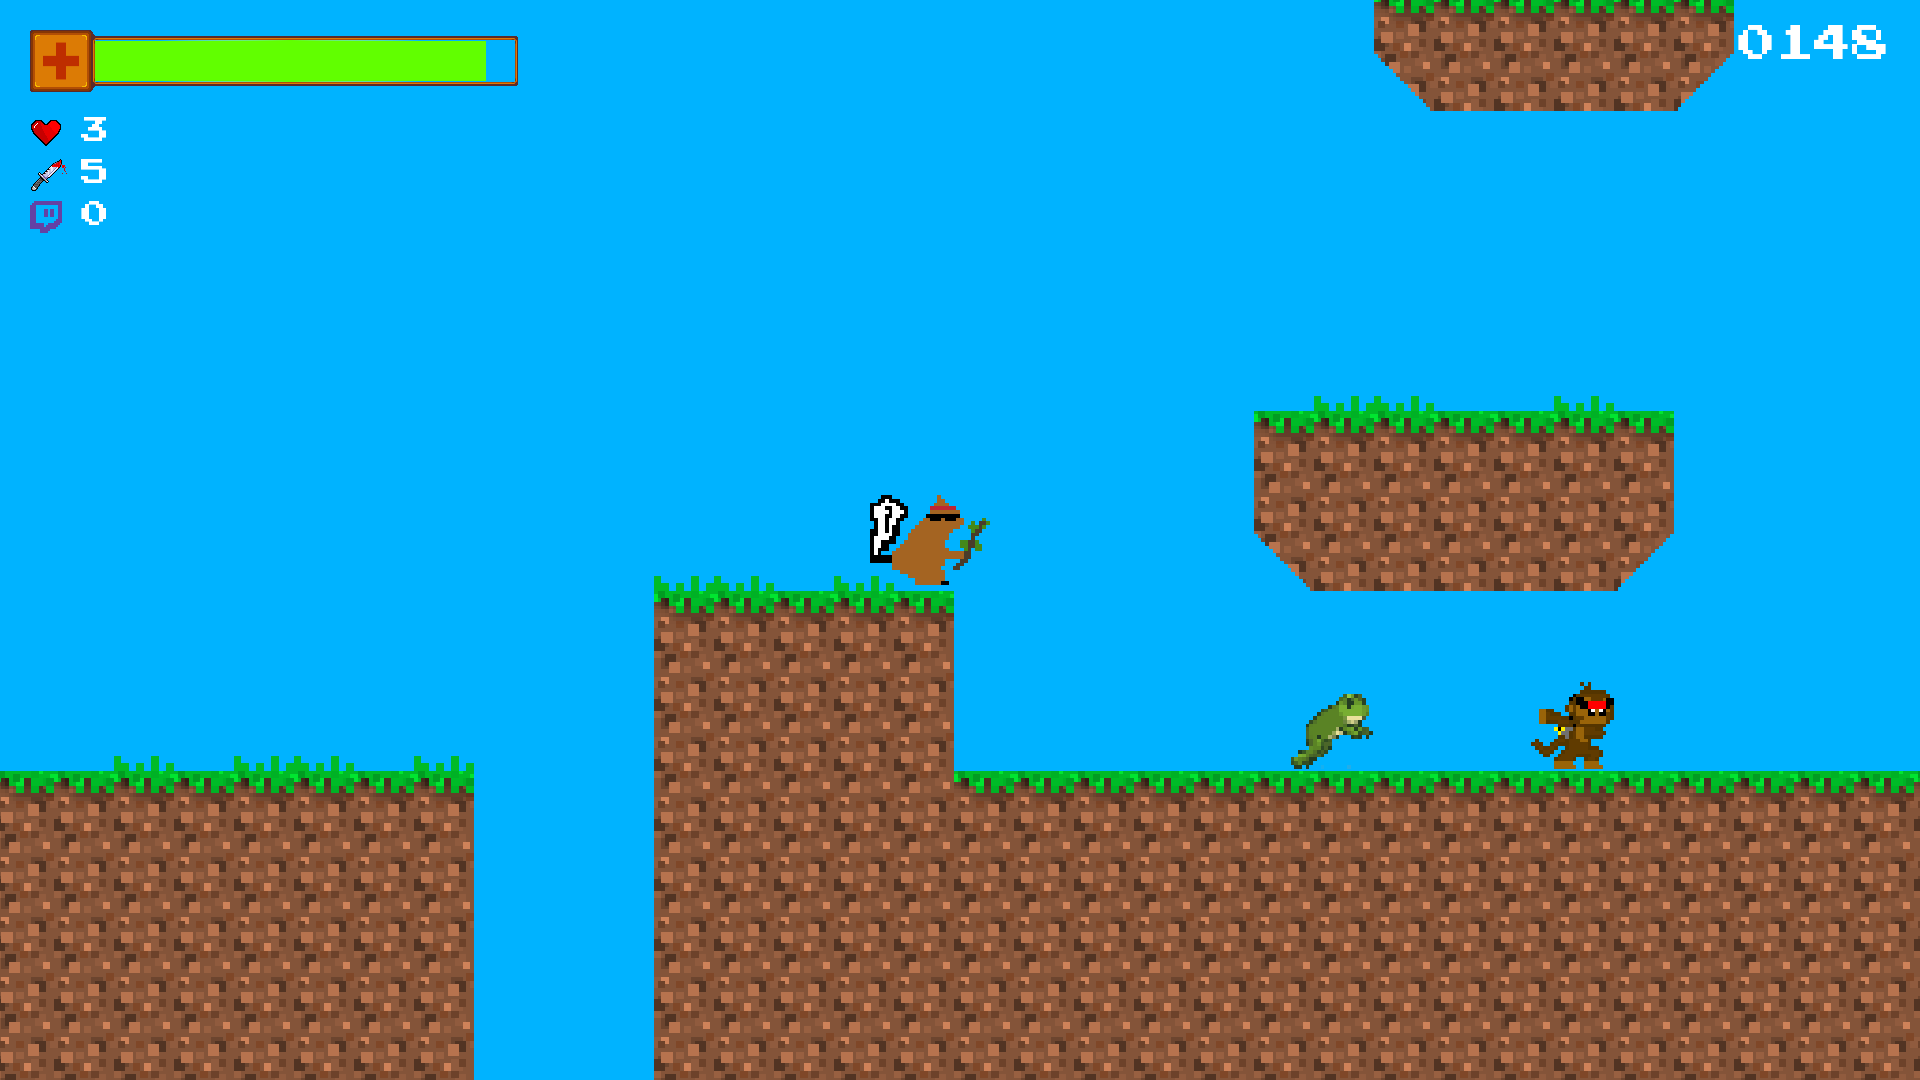
\includegraphics[width=1\textwidth]{screenshot.png}
 \caption{Screenshot of Gangster Squirrel}
\end{figure}

%----------------------------------------------------------------------------------------
%	METHODOLOGY
%----------------------------------------------------------------------------------------

\newpage
\section{Methodology} \label{Methodology}

\subsection{State of the Art}

To save time we decided to let each team member research a game they think fits closest to the concept of our game. We looked for 2D games, with a simple gameplay, that have retro styling. Each team member analysed their pick's features, platform support and price policy. At a team meeting we discussed what useful information we learned from our research and decided if it will be useful in our project.

\subsection{Business \& Marketing Strategy}
To enter the market and make our game competitive, we had to make a business and marketing strategy. In order to determine the best business strategy we had to analyze the models and strategies, and we chose to use the direct sales model.   

In the marketing strategy, we determined that we will not be distributing our game on the physical media, as many other companies have due to the extra cost's. Gangster Squirrel will be available solely online. Moreover, to aid with the advertising of our game, our marketing will be online, due to
its high return on investment, analytic capabilities and ease of use.

\subsection{Market Segmentation}
To have a successful game it is essential to have a market segmentation, so that the target group is established. In the marketing segmentation we shaped our target group via analyzing what kind of market segmentation suited them. Furthermore, we have used this information to build our business strategy as well. 

\subsection{Game Design}

To figure out the basic features of our game we did a qualitative analysis of the game \emph{Spelunky} \cite{Spelunky}, we wrote down the different features and elements we decided to include in our game. In terms of the look and feel of the game we looked more at retro games such as \emph{Super Mario Bros} published by Nintendo in 1985 \cite{SuperMarioBros}. To further investigate the design of our game we used quantitative research to examine what makes new retro games successful, we chose several games based on the features in the game and determined if any of those features could work in our game. We then wrote a list of all the main features of each game we looked at and decided what features we would like to implement in our own game. We also looked at what platforms would have the most potential for our game and compared the prices to the feature list of the other games to figure out how to price our own game.

\subsection{Documentation}
The approach we took for the technical documentation was to structure it a bit as a guide to build a game in Java. We tried splitting up the work we needed to do evenly amongst the team and each team member picked the sections they had the most knowledge about, so we could maintain a uniformly high level of detail. Each section was reviewed by a team member who hadn't written it, to make sure the explanations were understandable.

\subsection{Visual Documentation}
We made a subsection for each part of the game we had to design - the characters, maps, menu and head-up display of the game. Each item has its own subsection due to the different approaches we took to design each part of the game. 

\subsection{Technical Documentation}
We documented everything from choosing the libraries you might need, to animations, to integrating with third-part apps like Twitch. Each section contains both explanations of the functionality of the code, as well as snippets or external references to our code base on GitHub.

\subsection{Game Engine}

In order to determine the best game engine for our game, we did an analysis on various different Java game engines. We tried to find the most popular ones that aren't deprecated and researched their viability. We compared the learning curve of the different engines and looked at their features compared to what features we need in our game. We researched feedback from other developers who have used the game engines and came up with a list of different libraries that would be the best for the scope of our project. We did a quantitative analysis of the engines on our list and compared our results to determine which engine we should use.

\subsection{Playtesting}

To see if our implementation of our game concept was enjoyable, and if our market analysis gave us a reasonable price, we did a playtest of the game with a small group of test subjects. After playing our game the subjects answered a survey about which parts of the game they enjoyed, and which they enjoyed less, etc. We reviewed the data from the playtest to see where changes to our implementation and business model should be made. 

%----------------------------------------------------------------------------------------
%	STATE OF THE ART
%----------------------------------------------------------------------------------------

\newpage
\section{State of the Art} \label{sec:StateOfTheArt}
\subsection{Introduction}

% OLD STATE OF THE ART INTRO

% In this section, we have been looking for inspirations for our project. We have identified many of other games that are congruous to what we wanted to do. We were looking for our competitors via Google and we also knew a few of them beforehand. The Google search results we have found looking for key terms "2D mine games", "2D platform games" and similar. We picked the best-positioned examples and we chose the ones that are, in our opinion, the most similar and related to our game idea. Through this research, we wanted to get an overview of general features that this type of games has. Then we decided to discuss which of them were the most relevant and which we would like to implement. This section also helped us to understand the market that we are working in and decide what our pricing and platform support we should offer.

%------------------------------------------------

In this section, we have been looking at possible competitors which have a similar game concept as we do. The purpose of this is to determine strengths and weaknesses of these games and learn from their success or failure to create the best possible game ourselves, not only regarding the features and gameplay, but also the marketing, availability on different platforms and price.

The market for 2D side-scrolling games is basically infinitely large and not comprehensible in terms of picking the best games because there are too many. This is the reason, why we did not spend hours on searching for games on Google or the Steam charts or similar research possibilities, but rather decided to let each team member pick one game that he/she thinks fits best with the game concept that we brainstormed earlier and research that one game. Of course, we discussed each choice in the group and if everyone agreed that it was a good choice we made changes based on that discussion. Most games in the upcoming list were played by one or more team members previously, which made it easier and more accurate to determine it's main features, as well as good and bad points.

%------------------------------------------------

\newpage
\subsection{Our competitiors}

\subsubsection[Tallowmere]{Tallowmere \cite{Tallowmere}} \label{sec:StateOfTheArt_Tallowmere}

\begin{figure}[ht]
 \center
 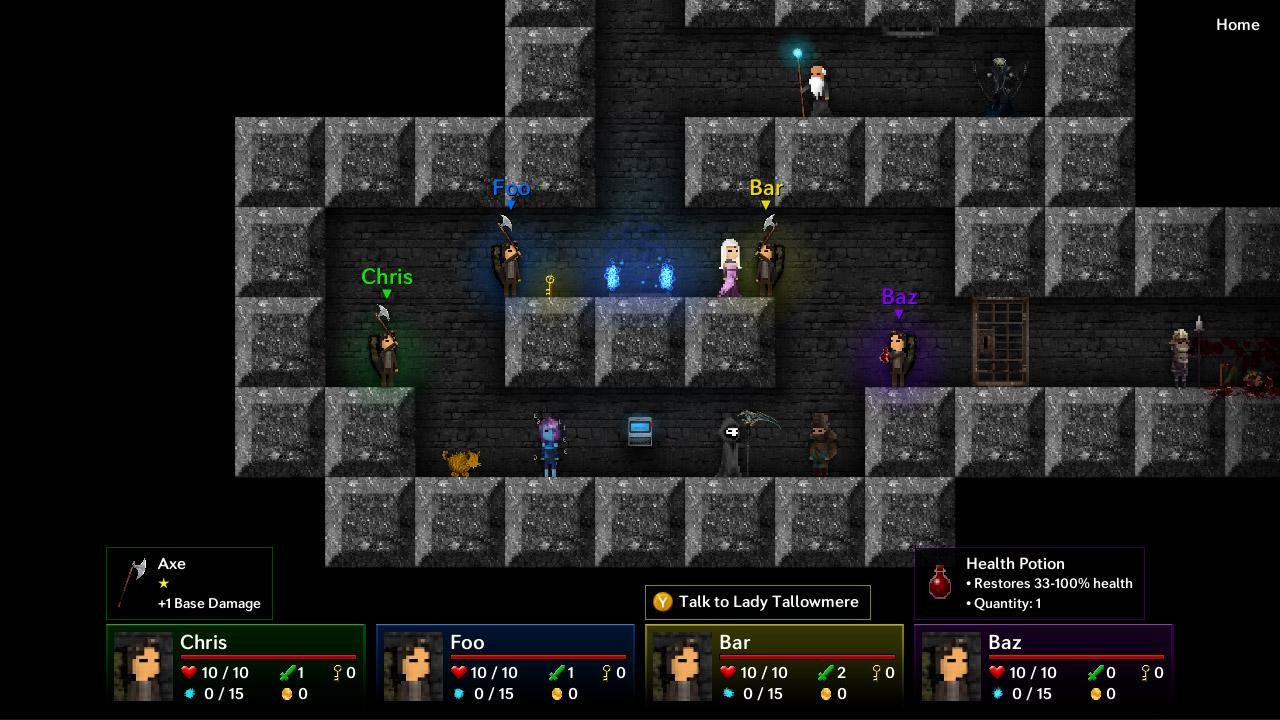
\includegraphics[width=0.8\textwidth]{StateOfTheArtScreenshots/tallowmere.jpeg}
 \label{sec:StateOfTheArt_Screenshots_Tallowmere}
 \caption{Screenshot of the game Tallowmere \cite{Tallowmere}}
\end{figure}

A 2D action platformer with an emphasis on executing your hero's jumping, shield-blocking, and weapon-attacking at the right moments as you move through a procedurally-generated dungeon.

Features:

\begin{itemize}
 \item Randomly-generated rooms, with each room bigger than the last
 \item Blood splats, particle effects and sounds
 \item Skill-based gameplay, with no ammo, mana, or stamina gauges
 \item Traps and obstacles to dodge and avoid
 \item Special boss and event rooms
 \item Different weapons, shields and garments the hero can equip
 \item Infinite jumping
 \item Single Player and local co-op (up to 4 players)
 \item Permanent death, with a typical run lasting from 1 minute to 2 hours depending on skill
\end{itemize}

Platforms:

\begin{itemize}
  \item Windows XP SP2 or newer
  \item macOS 10.8 or newer
  \item SteamOS
  \item Ubuntu 12.04 or newer
  \item Android 4.4 or newer
  \item iOS 8.1 or newer
  \item Wii U
\end{itemize}

Prices:

\begin{itemize}
 \item Steam: 3.99 EUR (4.71 USD)
 \item iTunes: 1.99 USD
 \item PlayStore: 16.0 DKK (2.54 USD)
\end{itemize}

Subconclusion:

We like the idea of a single hero that has to fight with enemies. Skill-based gameplay also appeals to us. We would like to get inspiration from their pricing system as well: the game is available on many different platforms and due to this, it has also varied prices.


%------------------------------------------------

\newpage
\subsubsection[Cave Story Plus]{Cave Story Plus \cite{CaveStoryPlusSteam}}

\begin{figure}[ht]
 \center
 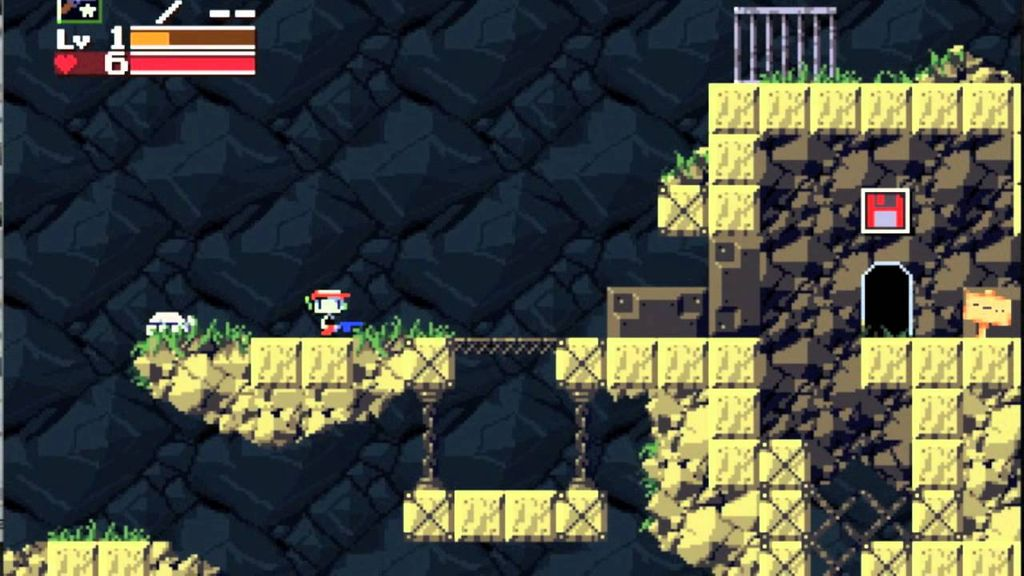
\includegraphics[width=0.8\textwidth]{StateOfTheArtScreenshots/cave_story_plus}
 \label{sec:StateOfTheArt_Screenshots_CaveStoryPlus}
 \caption{Screenshot of the game Cave Story+ \cite{CaveStoryPlusScreenshot}}
\end{figure}

Cave Story+ is a Cave Story remake for PC, Mac and Nintendo Switch developed by Nicalis, released in 2011. The game features remastered graphics and music as well as several new game modes, of which one is only made exclusively for the Nintendo Switch version \cite{CaveStoryPlusWiki}.

Cave Story+ has a selection of three difficulty levels; easy, standard and hard. Easy mode halves the HP of enemies and halves the damage they do to Quote (the main protagonist of Cave Story). The standard difficulty, is identical to the original game, in which Quote takes 100\% damage, and enemies have 100\% HP. Hard mode doubles the HP of enemies and removes all Life Capsules but one from the game, leaving the player with a maximum of 8 HP. Moreover, the Missile Launcher isn't available in the Hard mode.

Features:

\begin{itemize}
 \item Background music
 \item Over 20 boss battle games
 \item A variety of weaponry
 \item Four different game endings
 \item Hard mode for veterans
 \item Multiple versions available
 \item Metroid inspired setting
 \item Simple storyline
\end{itemize}

% REMOVE IF SOMETHING CHANGES
\newpage
% REMOVE IF SOMETHING CHANGES

Platforms:

\begin{itemize}
  \item Windows
  \item macOS
  \item Nintendo Switch
\end{itemize}

Prices:

\begin{itemize}
 \item Steam: 14.99 EUR (17.69 USD)
 \item iTunes: 4.99 USD
 \item Nintendo: 29.99 USD
\end{itemize}

Subconclusion:

The ideas that we like in this game are that enemies have various health points and that there are a few different weapons. As well as in this game, we would like to have our own simple storyline and background music.

%------------------------------------------------

\newpage
\subsubsection[Stardew Valley]{Stardew Valley \cite{StardewValley}} \label{StardewValley}

\begin{figure}[ht]
 \center
 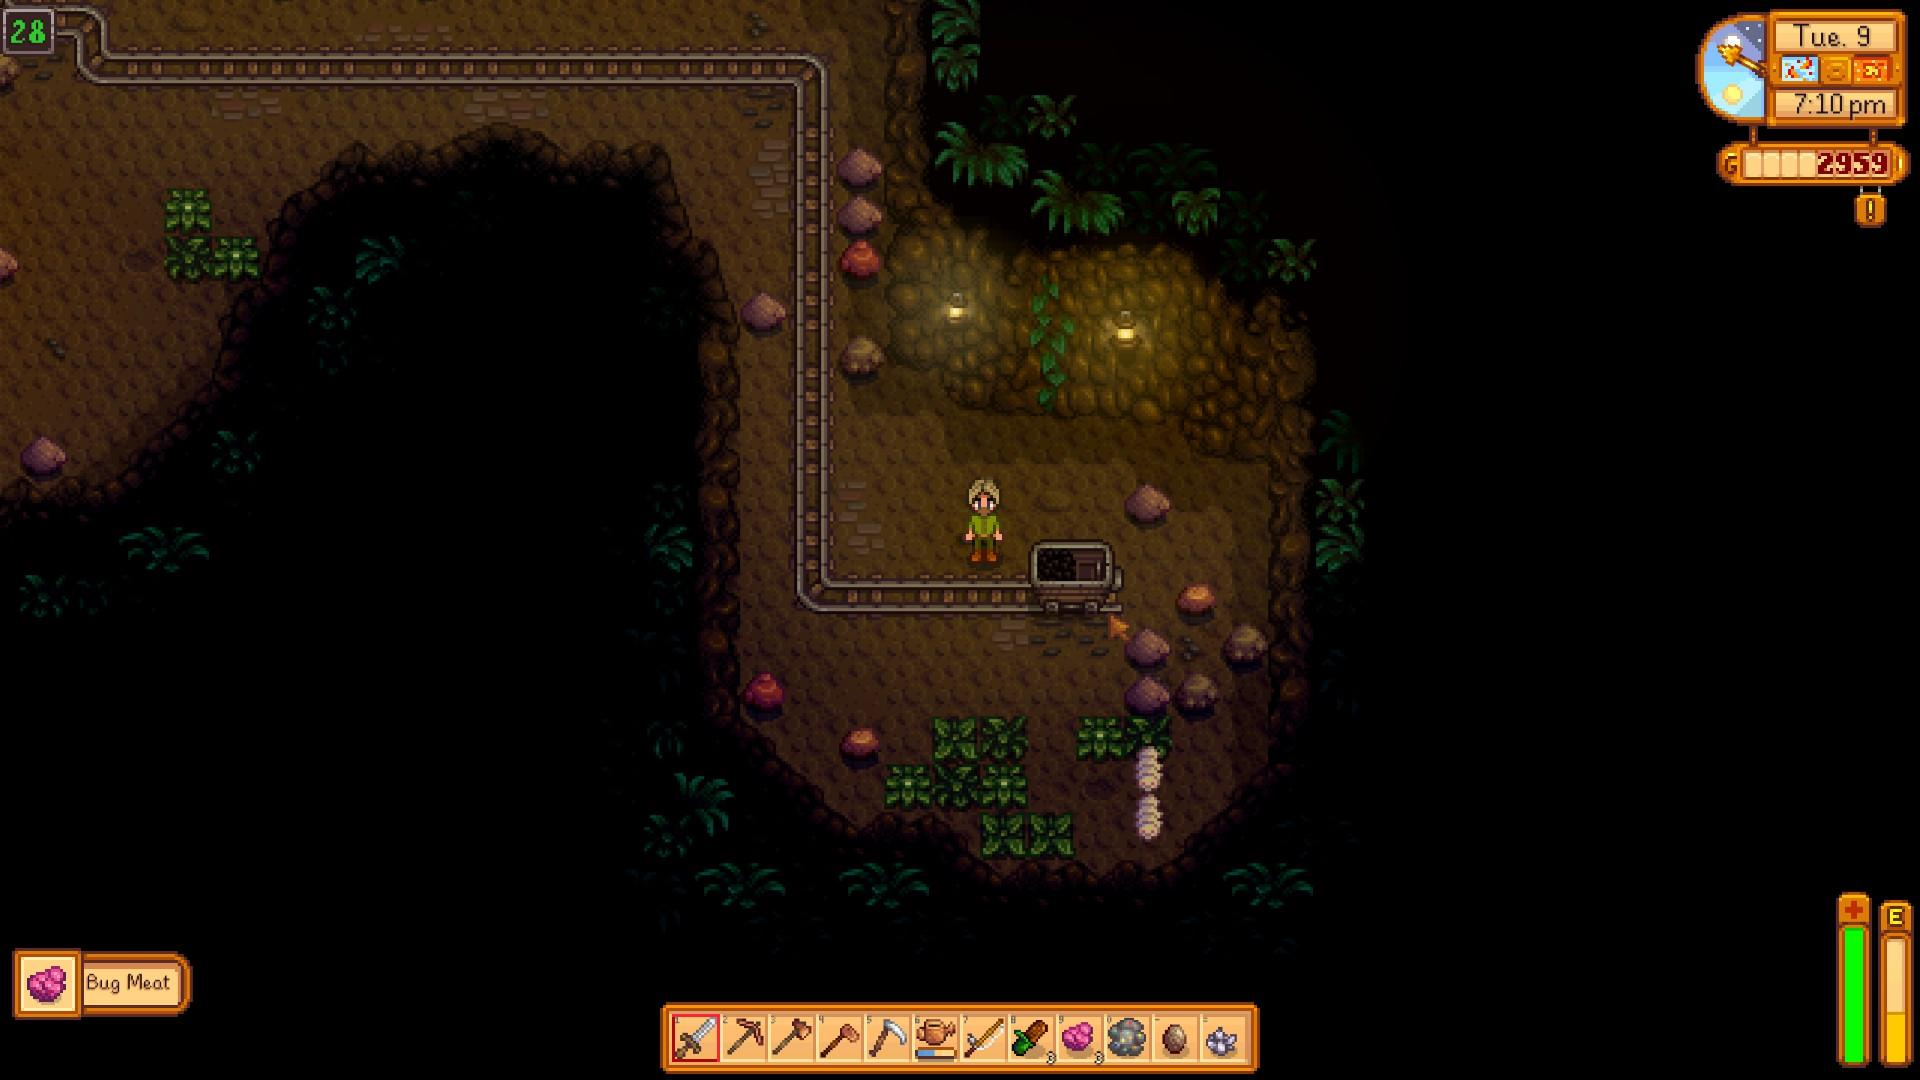
\includegraphics[width=0.8\textwidth]{StateOfTheArtScreenshots/stardew_valley}
 \label{sec:StateOfTheArt_Screenshots_StardewValley}
 \caption{Screenshot of the game Stardew Valley \cite{StardewValleyScreenshot}}
\end{figure}

Stardew Valley is a 2D top-down indie farming simulation, which features an endless mine, where the player can fight, gather resources for the character and his farm and explore the different levels. The mines consist of an endless amount of procedurally generated levels, with checkpoints after every five levels. These checkpoints can be reached by an elevator on the first level in the mines. Each level consists of several elements, which are mainly gatherable stones and enemies. Furthermore, some levels have special elements, which are quicksand, minecarts, chests, and more. To reach the next level, the player has to find a ladder down, which can be found under a random stone or ore. They can either be destroyed by a pickaxe or bomb. This mine system is only a small part of the overall game but offers a fun and highly replayable experience due to the infinite amounts of levels.

Features:

\begin{itemize}
 \item Top-down rather than a sidescrolling game
 \item Procedurally generated levels
 \item Different themes and enemies for different level regions
 \item Inventory system
 \item Health and energy system
 \item Upgrading of weapons and armor
 \item Resource gathering (for overall game)
 \item Simple 8-bit graphics with customizable character
\end{itemize}

% REMOVE IF SOMETHING CHANGES
\newpage
% REMOVE IF SOMETHING CHANGES

Platforms:

\begin{itemize}
  \item Nintendo Switch
  \item PlayStation 4
  \item Xbox One
  \item Windows
  \item Linux
  \item macOS
  \item PlayStation Vita
\end{itemize}

Prices:

\begin{itemize}
 \item Steam: 13.99 EUR (16.51 USD)
 \item Xbox: 14.99 USD
 \item Nintendo: 10.99 GBP (14.77 USD)
\end{itemize}

Subconclusion:

The concept that interested us the most in this game is the different theme on each level. The storyline is related in all of them, but the game world looks unlike on the other levels. Another feature that we would like to implement is similar to their player's health system.

%------------------------------------------------

\newpage
\subsubsection[Rogue Legacy]{Rogue Legacy \cite{RogueLegacy}}

\begin{figure}[ht]
 \center
 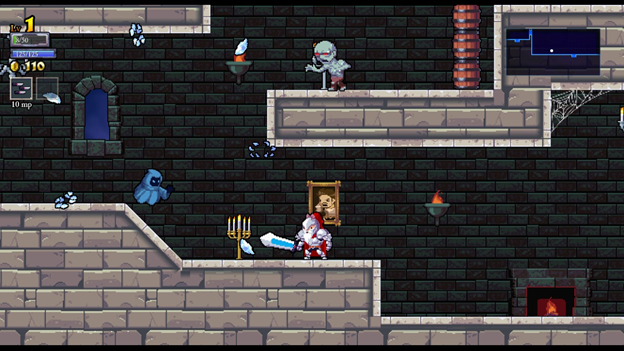
\includegraphics[width=0.8\textwidth]{StateOfTheArtScreenshots/rogue_legacy}
 \label{sec:StateOfTheArt_Screenshots_RogueLegacy}
 \caption{Screenshot of the game Rogue Legacy \cite{RogueLegacyScreenshot}}
\end{figure}

Rogue Legacy is a 2D game, which was released in 2013 and developed by Cellar Door Games. The game is about exploring a randomly generated dungeon and collecting gold. The player / character has default abilities such as jump and slash with a sword and secondary abilities such as magic attacks by using mana. The player has to defeat a boss in order to go to the next level \cite{RogueLegacyReview}.

Features: \cite{RogueLegacySteam}

\begin{itemize}
 \item Single player
 \item With sword, mana and life gauge to worry about
 \item Traps and obstacles to dodge and avoid
 \item More than 8 classes to choose from
 \item Over 60 different enemies
 \item Powerful weaponry and armor
 \item Tons of secret areas
 \item Boss in every stage
 \item Jump, run and dash
\end{itemize}

% REMOVE IF SOMETHING CHANGES
\newpage
% REMOVE IF SOMETHING CHANGES

Platforms: \cite{RogueLegacyWiki}

\begin{itemize}
  \item Windows
  \item Linux
  \item macOS
  \item PlayStation 3
  \item PlayStation 4
  \item PlayStation Vita
  \item Xbox One
\end{itemize}

Prices:

\begin{itemize}
 \item Steam: 14.99 EUR (17.69 USD)
 \item Xbox: 13.99 USD
 \item PlayStation: 16.99 USD
\end{itemize}

Subconclusion:

In this game, we like the boss idea the most. We would also like to have one really strong enemy to beat, but not on every level of the game - just on the last one. The prices for the game are in our opinion too high for a 2D platform game.


%------------------------------------------------

\newpage
\subsubsection[Mega Miner]{Mega Miner \cite{MegaMiner}}

\begin{figure}[ht]
 \center
 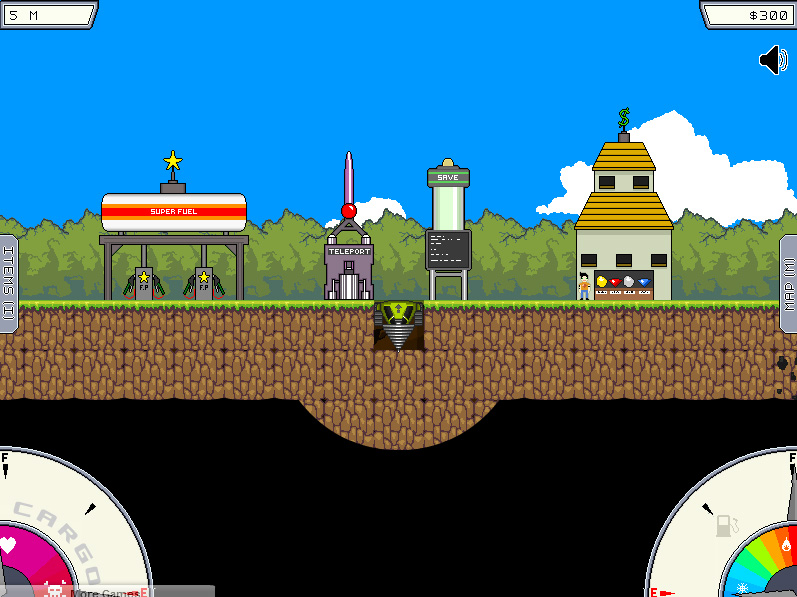
\includegraphics[width=0.8\textwidth]{StateOfTheArtScreenshots/mega_miner}
 \label{sec:StateOfTheArt_Screenshots_MegaMiner}
 \caption{Screenshot of the game Mega Miner}
\end{figure}

Mega Miner is a 2D game developed by Armor Games. The main task in the game is to drill a mine and while this process collects gold, silver, coal and other minerals. The player / character can then sell it for cash and upgrade his mining machine with new coolers and more. This game is qualified as a strategy game.

Features:

\begin{itemize}
 \item Single player
 \item Gold, silver, coal and other minerals to collect
 \item Rocks as obstacles to avoid
 \item One map
 \item No enemies
 \item Possibility to upgrade character (drill)
\end{itemize}

Platform: 

\begin{itemize}
  \item Adobe Flash Player
\end{itemize}

Price: Free

Subconclusion:

From this game, we received inspiration for collecting resources. However, due to our time limits, we were not sure if we will be able to implement this feature, so we decided to treat it as a subsidiary idea. Also, the fact that the game is available for free made us sure that the price for our game should not be too high.


%------------------------------------------------

\newpage
\subsubsection[Spelunky]{Spelunky \cite{Spelunky}}

\begin{figure}[ht]
 \center
 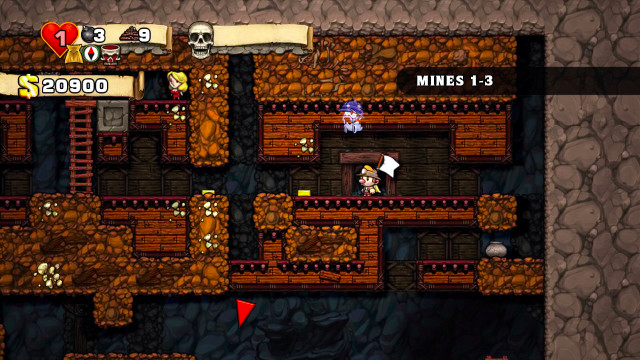
\includegraphics[width=0.8\textwidth]{StateOfTheArtScreenshots/spelunky}
 \label{sec:StateOfTheArt_Screenshots_Spelunky}
 \caption{Screenshot of the game Spelunky \cite{SpelunkyScreenshot}}
\end{figure}

Spelunky is a 2D cave exploration/treasure-hunting game inspired by classic platform games such as Rayman, Super Mario, and Sonic the Hedgehog. One of the crucial features that differentiate this game to the classic versions, is that the game is top-down rather than sidescrolling, which leaves the player with a completely different feel. With an inventory full of bombs, ropes, and your own whip, the aim is to creatively maneuver through the fully-destructible ancient caves. In order to complete levels, you have to search deep in the underground for a door, while encountering a variety of enemies, as well as traps and treasure. It's a challenging game that will likely test your patience since you will die continuously. But with many deaths comes experience, and eventually, as you beat the level, the frustration is overtaken by a great feeling of satisfaction.

\textbf{Pros and Cons:}

\textbf{Pro:} Skill based gameplay. \emph{In Spelunky the player has everything needed from the start so it is only the skill level of the player that determines whether you advance or not.}

\textbf{Pro:} Roguelike genre allow for quick sessions. \emph{Since the gameplay is so quick, the player will die quite often which means that the sessions tend to be quite short. This makes for a game that can be played in quick bursts throughout the day.}

\textbf{Con:} No check-point system. \emph{You can't save the game and you can't go back to a level with your previous equipment.}

\textbf{Con:} Hard to master. \emph{The game is difficult to the point of frustration.}

% REMOVE IF SOMETHING CHANGES
\newpage
% REMOVE IF SOMETHING CHANGES

Features:

\begin{itemize}
 \item Top-down rather than a sidescrolling game
 \item Skill-based gameplay
 \item Single player and local co-op (up to 4 players)
 \item Traps and enemies to dodge and avoid
 \item Inventory system primarily with bombs and ropes
 \item Money collecting for the shopkeeper in-between levels
 \item Full maneuverability with infinite jumping and running
\end{itemize}

Price: Free

Subconclusion:

This game has the storyline a bit deviating from ours, but despite this, we used it to get to know better our game idea. We like that it is top-down - we decided to implement it on our second level in the game. About the price - the number of features in this game and that it is free to play once again confirmed that our price should be relatively low.

%------------------------------------------------

\newpage
\subsubsection[Nuclear Throne]{Nuclear Throne \cite{NulcearThrone}}

\begin{figure}[ht]
 \center
 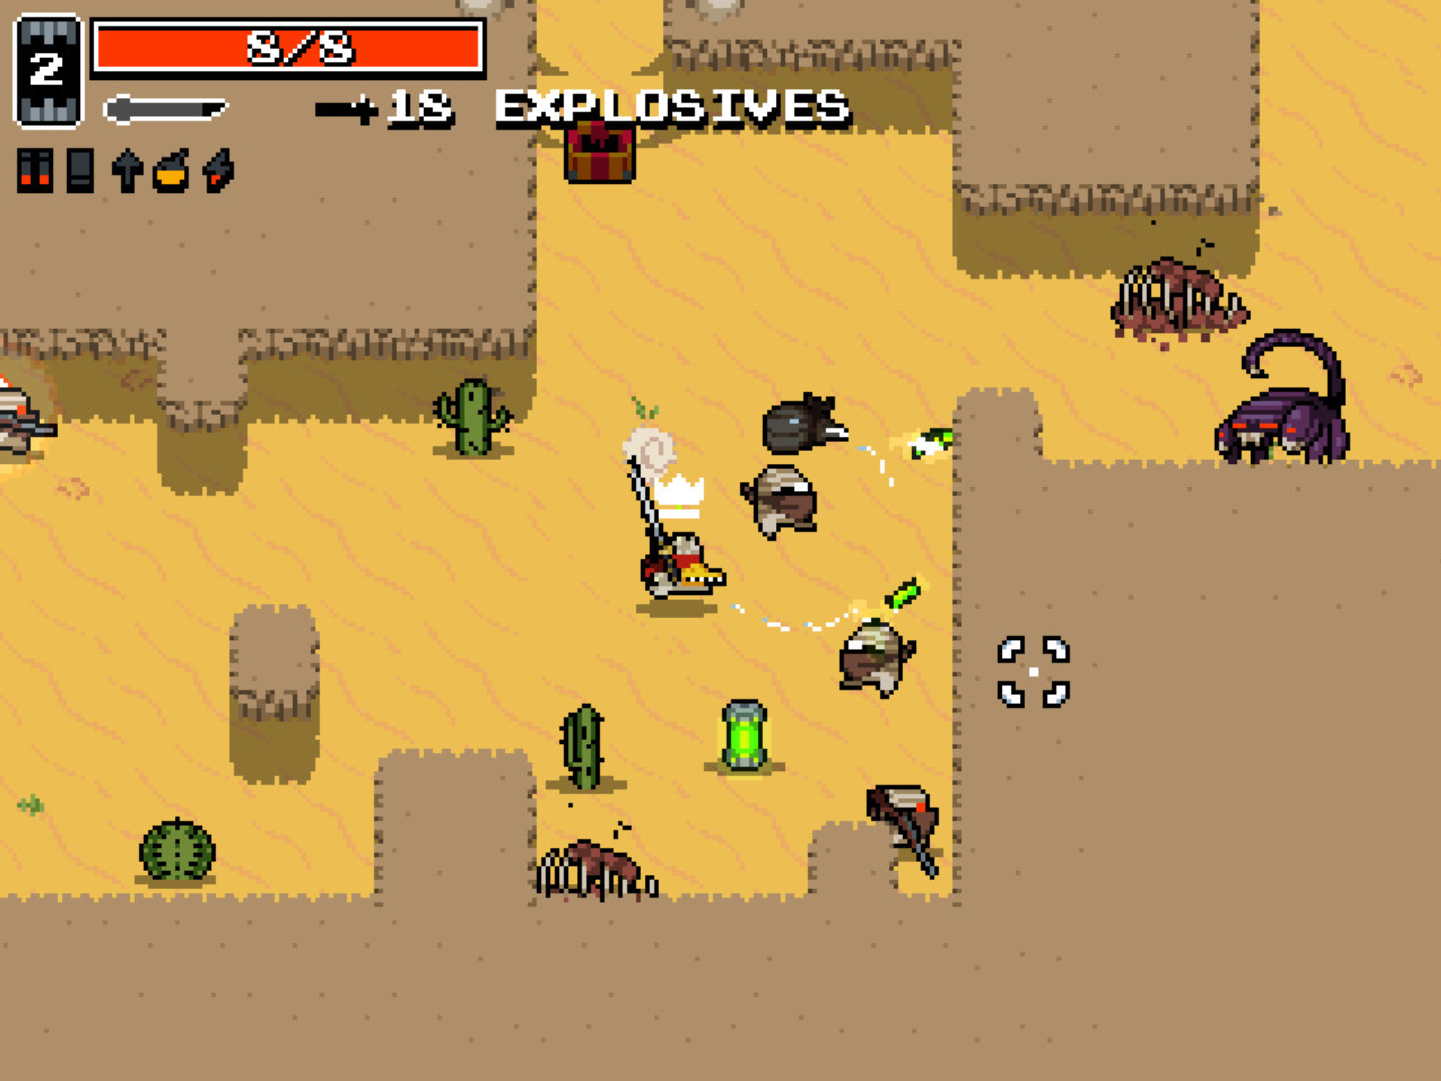
\includegraphics[width=0.8\textwidth]{StateOfTheArtScreenshots/nuclearthrone}
 \label{sec:StateOfTheArt_Screenshots_Nulcearthrone}
 \caption{Screenshot of the game Nuclear Throne \cite{NulcearThroneScreenshot}}
\end{figure}

Nuclear Throne is a "bullet hell" 2D top-down shooter, with an 8-bit retro style look and feel to it. The gameplay is very simple, there are different weapons you can pick up throughout the game, progressively getting better weapons as you play the game. The game consists of several themed "worlds", featuring themes such as desert, frozen, sewer. Each world has several levels where you face enemies shooting hundreds of projectiles at you, which is why it's referred to as a "bullet hell" game. At the end of each world, you must fight a boss before you can advance to the next world. The game also features multiple characters you can play in each playthrough.

Features:

\begin{itemize}
 \item Top down view
 \item Multiple themed worlds
 \item Multiple boss battles
 \item A large variety of weapons
 \item Multiple characters
 \item Procedural levels
 \item Daily challenges
\end{itemize}

Prices:

\begin{itemize}
 \item Steam: 11.99 USD
\end{itemize}

Subconclusion:

What captivated us the most in this game is the retro style of it. Also, there are many ideas that have already appeared in previous games that we like: different weapons, themes and the level with a boss to beat.

%------------------------------------------------

\newpage
\subsection{Conclusion}

The games research that we made helped us to establish what features Gangster Squirrel should have and also to better understand how the gaming market looks like. The list below shows the features that we agreed on:

\begin{itemize}
  \item Single player
  \item 2D platform game
  \item 3 non-randomly generated levels (the last one should be with a Boss)
  \item One version supported - Desktop
  \item Squirrel as a hero
  \item Matching environment - the outside world, tree, the interior of the tree
  \item Matching enemies - frogs, monkeys
  \item Hero has limited lifes and health points 
  \item Variety of weapons
  \item Background music
\end{itemize}

\textbf{Platforms:}

We would like our game to be available on at least all of the platforms our competitors have released their games for, but due to our time limitation, we decided to first implement a desktop version and then expand it to others, if possible.

\textbf{Price:}

As we mentioned in subconclusions above, many games that are similar to what we want to do are for free, so the price for our game should be relatively low. The price range for the desktop versions of the games that we researched is 0 - 30 USD, so we will try to find a fair price considering the number of features that we will implement.

%----------------------------------------------------------------------------------------
%	MARKET ANALYSIS
%----------------------------------------------------------------------------------------

\newpage
\section{Business Strategy} \label{MarketAnalysis}

\subsection{Business Model} 
Ever since the release of Pong \cite{Pong} in the U.S. and the beginning of the first generation of video game consoles in 1972 the gaming industry has been growing steadily and sees no end in sight. It has spread throughout the globe and game development companies have become international organizations. The only part of the globe where games are not popular is South America \cite{GamesMarketRevenue}. In the past few years, the mobile gaming segment has overtaken all others in revenue and is expected to increase its lead over the coming years.

\begin{figure}[ht]
 \center
 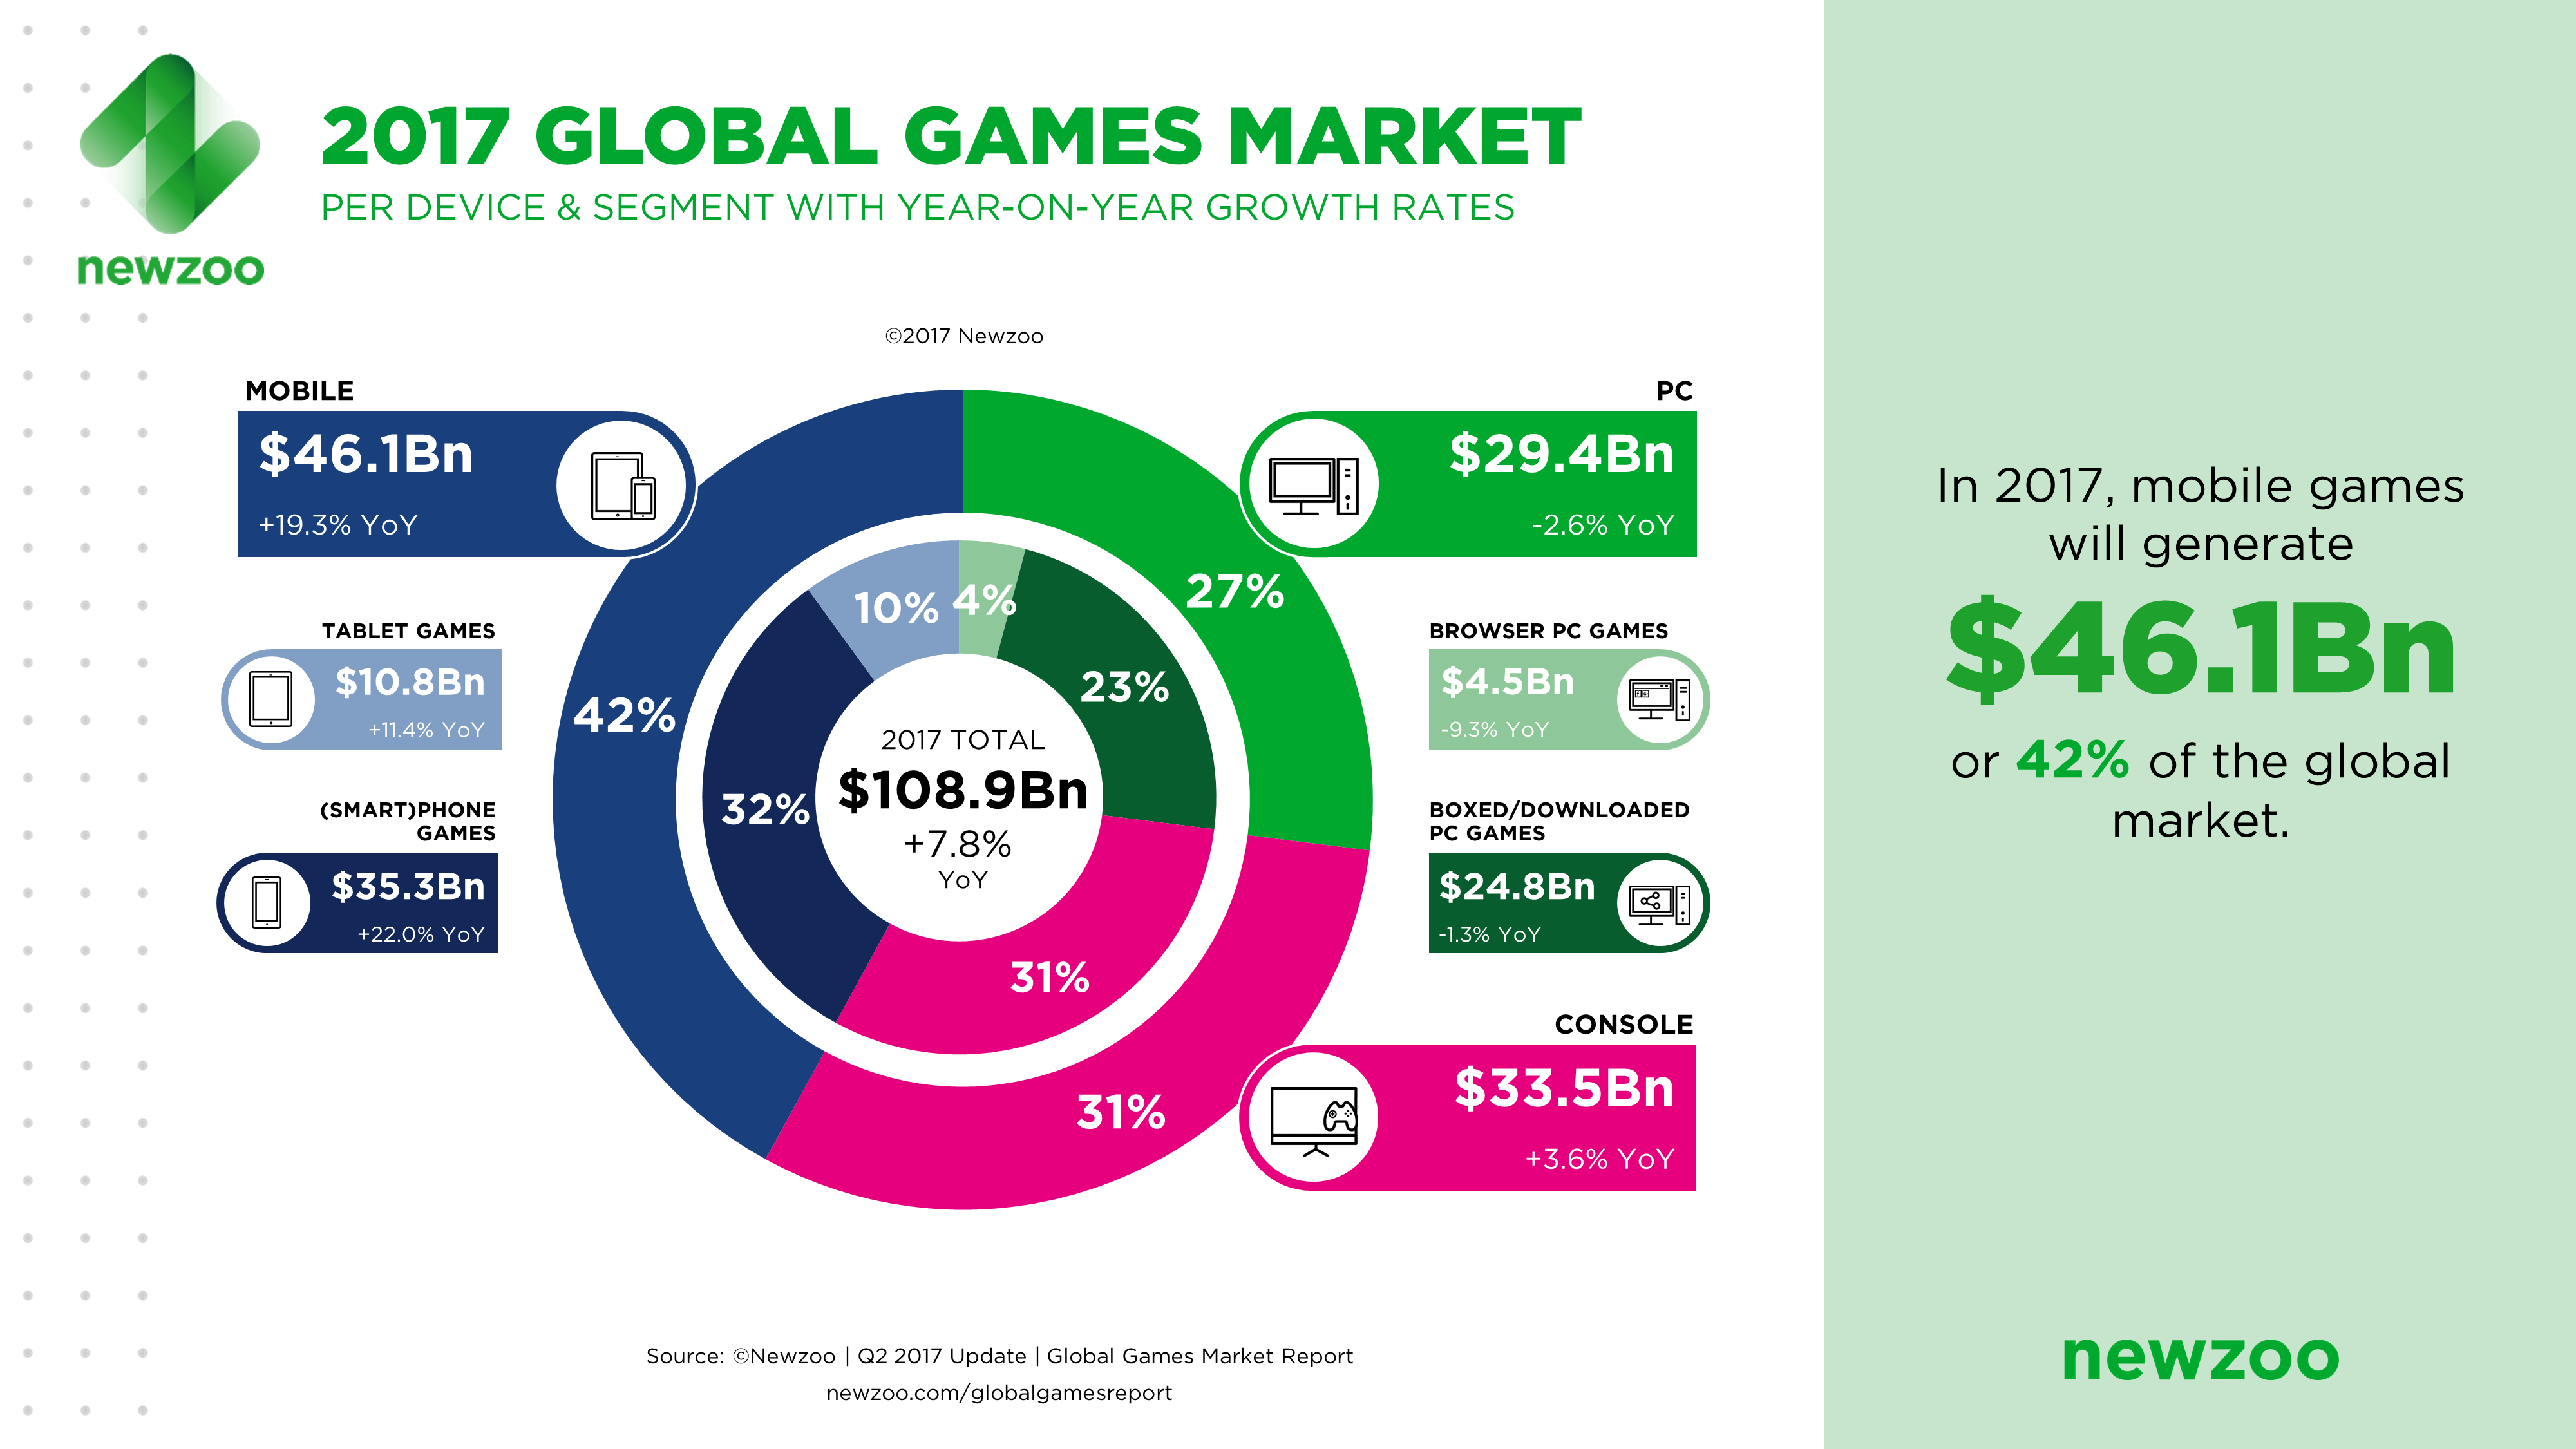
\includegraphics[width=1\textwidth]{BusinessStrategy/Newzoo_2017_Global_Games_Market_Per_Segment_April_2017}
 \label{Newzoo_2017_Global_Games_Market_Per_Segment_April_2017}
 \caption{Newzoo 2017 Global Games Market Per Segment \cite{NezooScreenshot}}
\end{figure}

One of the reasons for this growth is the inclusion of new players - mostly females and elders, has induced the popularity of casual games in social networks and mobile apps. Another reason is the constant development of the different business models used by game developers. The most successful in recent years has been the free-to-play-model \cite{BusinessModelsAndStrategy}.

So how to combine these strengths into a model that will help us establish our project in this competitive market?

We plan to use the trends in gaming to our advantage - PC games are still popular, but players expect an impressive gaming experience in return for their money. Mobile games are growing in popularity and lots of people are happy to pay for a simple entertaining experience.

Therefore we plan to release the first level of Gangster Squirrel for free for Mobile and Desktop devices as an effort to boost interest. The full-length game will be available on mobile for 1.99\$ USD and desktop for 3.99\$ USD. These prices make our game competitive with our competitors, many listed in section \ref{sec:StateOfTheArt}.

A subscription-based model, though other games have had great success with it, doesn’t make sense in our case, because our game is very short. We plan to build a strong brand with successful sequels of the game, which will help with establishing ourselves in the market.

\subsection{Marketing Strategy}

Through the long history of game development, the marketing utilized by game producers has been quite varied \cite{MarketingStrategyExamples}. Users have been bombarded with promotional videos, print ads, billboards, newsletters and much more. Some companies have benefited from their marketing materials going viral.
Our game will not be distributed on physical media, due to the added cost, it will be available solely online. Therefore to aid with the advertisement our marketing will also be online, due to its high return on investment, analytic capabilities and ease of use.

%------------------------------------------------

\subsection{Market Segmentation}

Market segmentation is the process of dividing a broad consumer or business market, normally consisting of existing or potential customers, into sub-groups of consumers which are known as segments. The segments are based on some type of characteristics. Which typically are common characteristics, such as shared needs, common interests, or similar lifestyles. Market segmentation has become critical to any business or marketing plan \cite{MarketSegmentation}.

The market is highly competitive as major vendors are competing against each other to acquire a greater market share. As specified further under the “Business Model” section in the report, there has been a peak in the past few years in mobile gaming, which has opened up the doors for new players - mostly females and elders have induced the popularity of casual games in social networks and mobile apps. The statistic below shows the gender split among U.S. computer and video games from 2006-2017. Moreover, the calculation showed that nearly 42\% of all gamers in the United States, were women, a slight increase over the previous year. Based on a 2015 forecast, worldwide video game sales have increased to nearly 75 billion U.S. dollars in 2015 and are expected to grow to 90 billion by 2020. In 2014, it was also calculated that there were some 1.8 billion gamers in the world, which equals to about 25 percent of the entire global population. Therefore, video gaming is not only a hobby or for entertainment. It is the basis of a tremendous industry, worth over tens of billions U.S. dollars \cite{VideoGamerGender}.


\newpage
\begin{figure}[ht]
 \center
 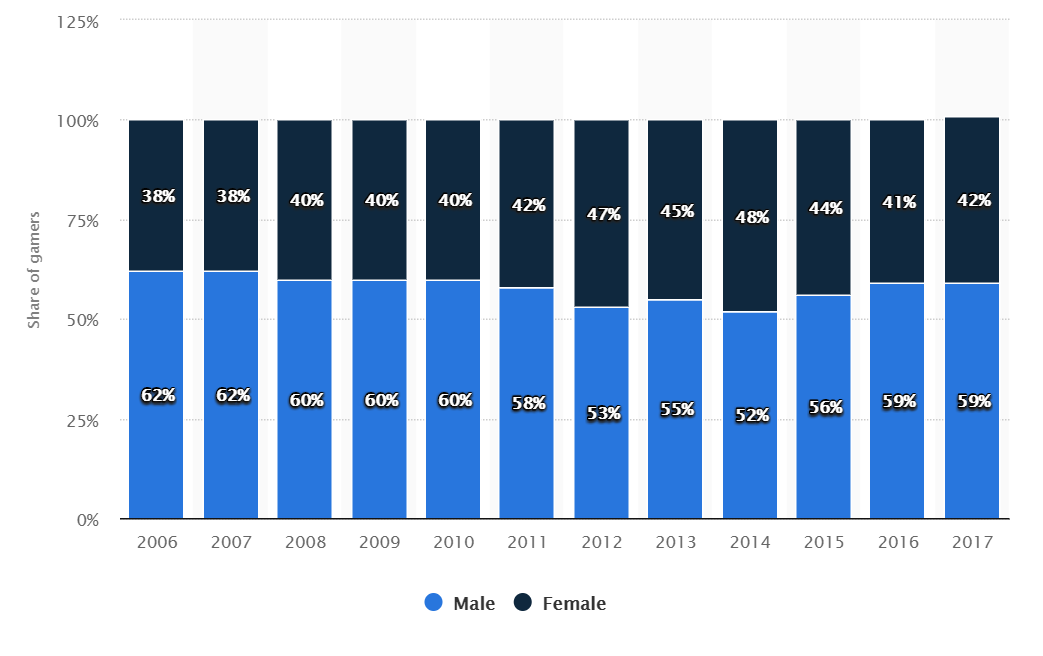
\includegraphics[width=1\textwidth]{BusinessStrategy/Statistics-MarketSeg}
 \label{Statistcs-MarketSeg}
 \caption{Distribution of computer and video gamers in the United States from 2006 to 2017, by gender \cite{NezooScreenshot}}
\end{figure}

Today, 27 percent of U.S. video gamers are between the ages of 18 and 35, so roughly every third game enthusiast is a Millennial, with figures going further towards the younger generation in recent years. However, 26 percent of surveyed Americans who admitted having playing video games were at least 50 years old \cite{VideoGamerGender}.

There are four basic market segmentation-strategies which are based on: 

\begin{itemize}
  \item behaviour
  \item demographic
  \item geographical differences
  \item psychographic
\end{itemize}

Segmentation according to demographic is based on consumer-demographic variables such as age, income, family size, economic status etc. This kind of segmentation assumes that consumers with similar demographic profiles will exhibit similar purchasing patterns, and have similar interests, lifestyles and motivations. Moreover, that these characteristics will translate into similar product/brand preferences. The demographic segmentation is one of the simplest and widest types of market segmentation used. 

Behavioral segmentation divides the population on the basis of their behavior, usage and decision-making pattern. For example, young people will always prefer a smartphone whereas elder people will prefer a standard cellphone. This is an example of behavior based on segmentation. The product is marketed, by the behavior of an individual. 

Geographical segmentation divides people on the geographic criteria. The potential customers will have different needs based on the geography they are located in. In practice, markets can be segmented as broadly as continents and as narrowly as neighborhoods or postal codes. This type of segmentation is the easiest but it was actually used in the last decade where the industries were new and the reach was less.

The psychographic segmentation is one which uses lifestyle of people, their interests, activities, and hobbies as well as opinions to define a market segmentation. It’s quite similar to the behavioral segmentation. But psychographic also takes the psychological aspects of consumer buying behavior into accounts. Having the statistics and latest Games Market Report in mind, we have chosen to limit our target group to consumers aged between 18-50 years old, and to categorize our segmentation as psychographic \cite{MarketSegmentation}.

Our segmentation is generally based on gamers, who have interest in retro gaming. We target people who want to bring the old retro games back on the market. There is a slight decreasement in the Boxed/Downloaded PC Games for this year. However, there has been an immense growth in mobile gaming, throughout the past few years. Which will eventually make the market size expand for the years to come. One thing our customers have in common is retro gaming, whether it's for a small platform (mobile gaming) or a big platform (PC-games). Segmentation basically divides a population based on variables. We believe that our target group will be suitable for the psychographic market segmentation-strategy.  

The latest quarterly update of the Global Games Market Report, released by Newzoo, displays the essence of computer gaming. Throughout the infographic, is illustrated the big part computer gaming has on the global games market since 2016 and will have until est. 2020. Having this in mind we have chosen to release Gangster Squirrel for free for Desktop devices as an effort to boost interest. The full-length game will be available for 3.99\$ for the desktop. Furthermore, if the desktop-version succeeds, a mobile version will be available as well for 1.99\$

\begin{figure}[ht]
 \center
 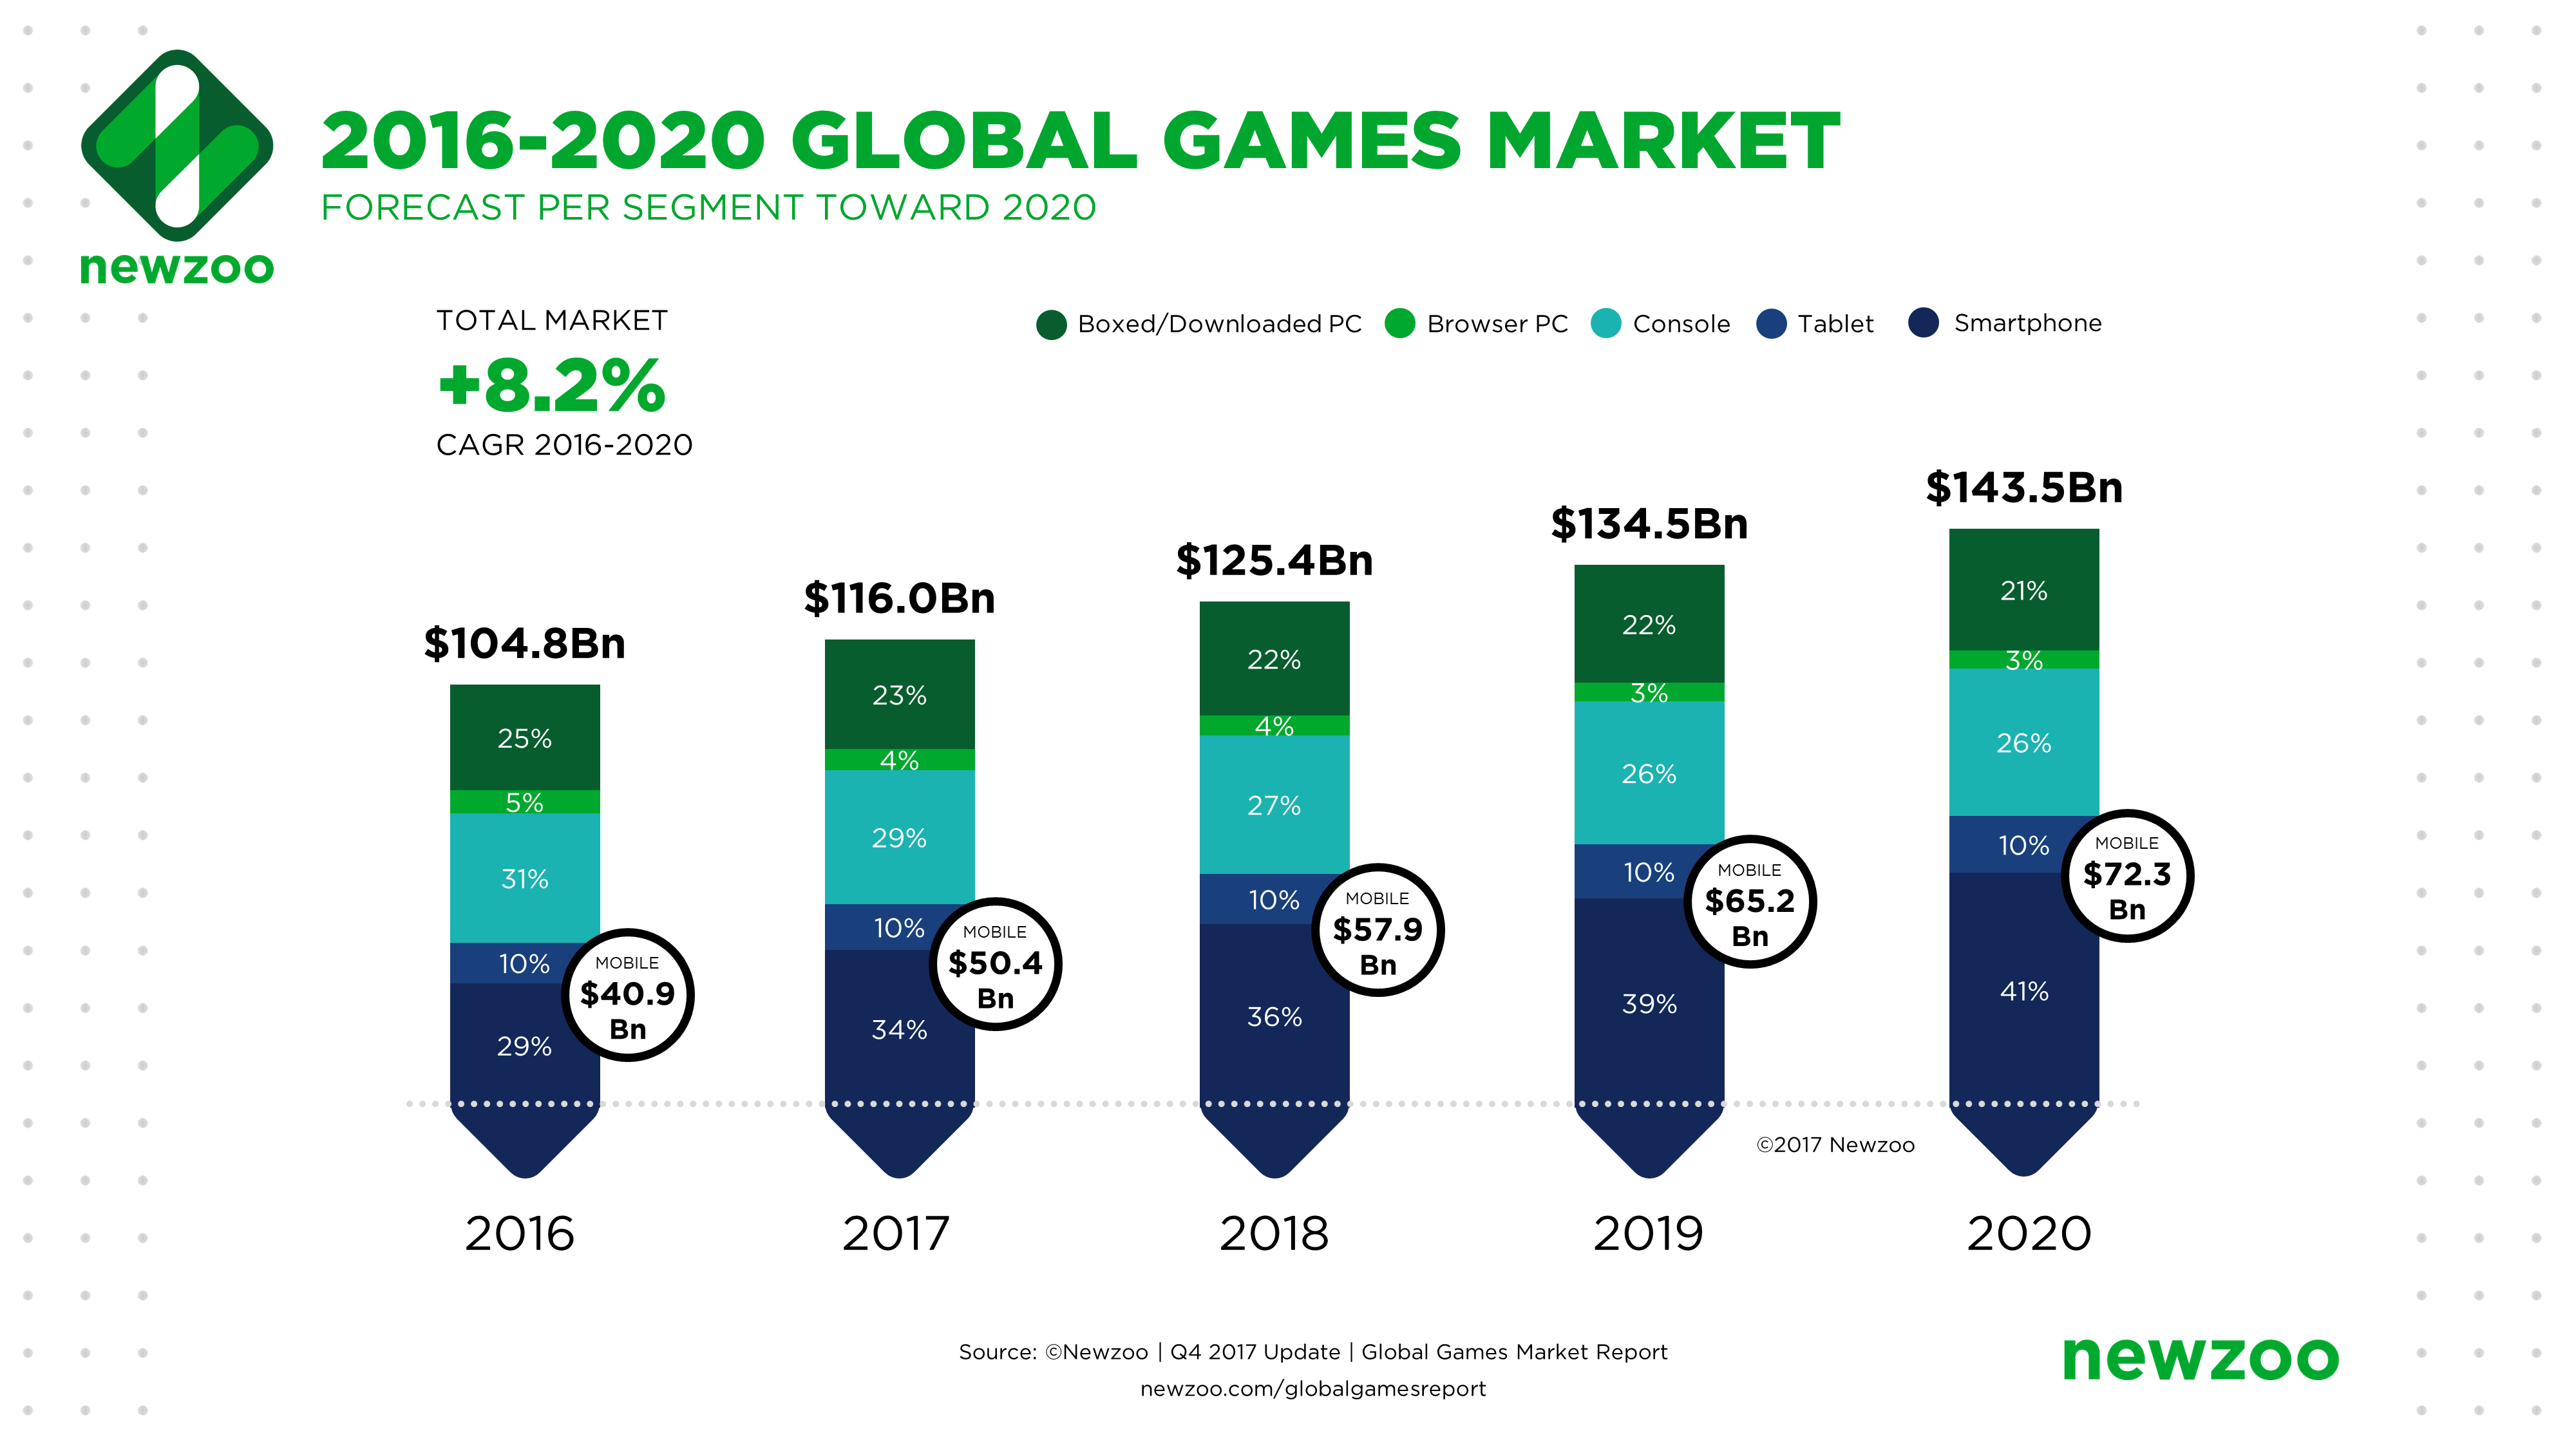
\includegraphics[width=1\textwidth]{BusinessStrategy/GlobalGamesMarket2016-2020.png}
 \label{GlobalGamesMarket2016-2020}
 \caption{2016-2020 Global Games Market (forecast per segment toward 2020) \cite{GlobalGamesMarket}}
\end{figure}

%----------------------------------------------------------------------------------------
%	VISUAL DOCUMENTATION
%----------------------------------------------------------------------------------------

\clearpage
\section{Visual Documentation} \label{VisualDocumentation}

\subsection{Player textures} \label{DocVisualPlayerTextures}

Since our original idea of the game and the main character was ludicrous, we realized that we wouldn’t find any finished game concepts with all the accessories and features that we desired. Instead, we decided to figure out the look of the squirrel, as well as brainstorming accessory-clothing and weapons that we found fitting for the overall theme of the game.

Since the original idea was that we wanted to do custom textures for every character in the game, we made sure to research the general opinion on both software and online solutions for making 8-bit textures. Logically, it quickly came apparent that downloaded software is the superior option, as they allow for more advanced features, as well as adding animation. According to our research it came clear, that the general opinion is that \emph{PyxelEdit} \cite{PyxelEdit} and \emph{GIMP} \cite{GIMP} are the best free options, so the group members decided to use one of these depending on preference.

The main character was created with PyxelEdit, since the program allows for easy and simple tile creation, which made it painless to insert the regular squirrel and add a different weapon for each tile, as shown in the picture underneath.

\begin{figure}[ht]
 \center
 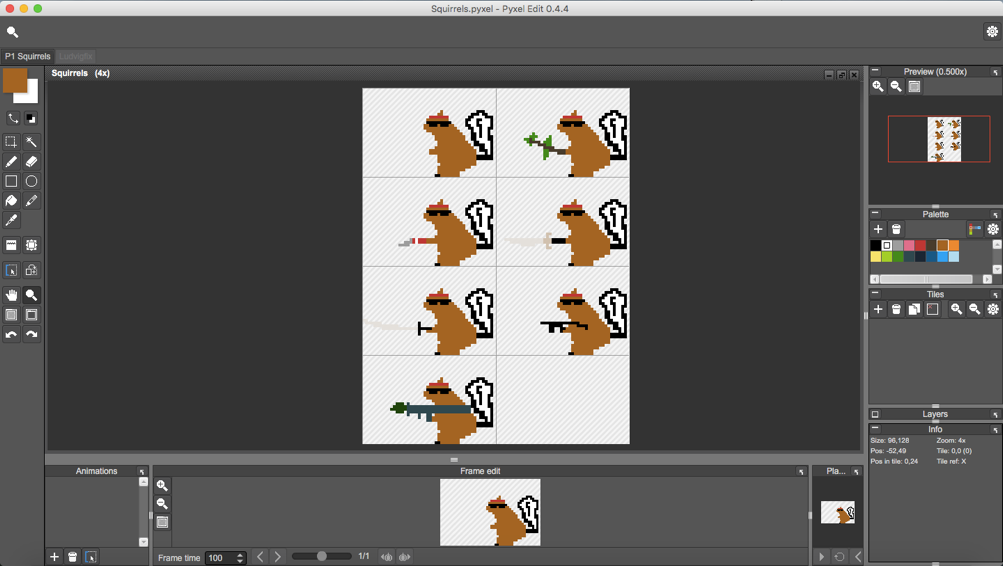
\includegraphics[width=1\textwidth]{Documentation/Picture1.png}
 \caption{PyxelEdit interface \cite{PyxelEdit}}
 \label{fig:pyxeledit_screenshot}
\end{figure}

\newpage 
The look of the squirrel was done with inspiration from the “White-tailed Antelope Ground Squirrel”. The weapons are made with inspiration from the weapons listed chronologically below:

\begin{itemize}
  \item Branch
  \item Swiss-Army Knife
  \item Switchblade
  \item Katana
  \item Tommy Gun
  \item Rocket Launcher
\end{itemize}

As it appears, some of the peculiar details were lost when trying to recreate the weapons, as 8-bit textures have its delimitations. 

The attacking animations were done with the same approach as any other animation in our game. In this particular case, it is only done with a single different texture with the weapon stretching out from the body of the squirrel, as shown in the image below.

\begin{figure}[ht]
 \center
 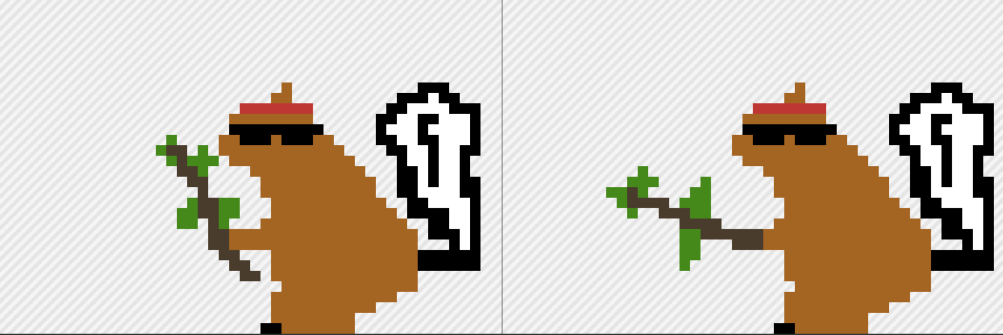
\includegraphics[width=1\textwidth]{Documentation/Picture2.png}
 \caption{The default and attack texture of the squirrel holding a branch}
 \label{fig:squirrel_branch_default_attack_texture}
\end{figure}

\newpage 
\subsection{Enemy textures}

We wanted to be in complete control of the actual look of characters, and although it would be ideal to have our own design for every enemy as well, we quickly realized that this would be a time-consuming process, so we decided to research different possibilities. The group decided to research the web for finished designs for enemies, and it quickly came apparent, that there’s a plenitude of animated 8-bit GIF’s (Graphics Interchange Format) available online. 

We decided not to have an excess number of enemies, as it could ruin the playing experience, as well as being time-consuming to implement. We went with only three enemies, a frog \cite{FrogEnemyDesign}, a bird \cite{BirdEnemyDesign} and a monkey \cite{MonkeyEnemyDesign}, as well as a boss \cite{BossEnemyDesign} at the end of the third level, as we felt like that would be the suitable amount to also make room for other features. 

All the three added enemies are GIFs. A GIF is a bitmap image format, which basically is a series of images composing an animation in a loop.

An image of the spritesheet of the frog enemy can be found in the animation section (\ref{DocAnimations}).

\subsection{Maps} \label{VisualDocMaps}

\subsubsection{Map textures}

The textures are the graphical images by which one can construct the whole map. In order to make a map for our project, we needed to make some textures / spritesheets, for example for the player (squirrel), the ground, background, and weapons. We made the spritesheets / textures by using the web-application piskelapp \cite{piskelapp}, which allows the users to draw the textures according to their requirements. We also used some premade textures from a website called opengameart \cite{opengameart}, which provides a large variety of free textures.

\subsubsection{Map creation}

A game's map has a huge influence on the game experience, since it's the environment that the player is gonna manoeuvre around in. Gangster Squirrel consists of three levels (maps).

\begin{itemize}
 \item The first level is on the ground, where the player has to go from left to right to find his way to the next level (see figure \ref{fig:FirstLevel}).
 
\begin{figure}[ht]
 \center
 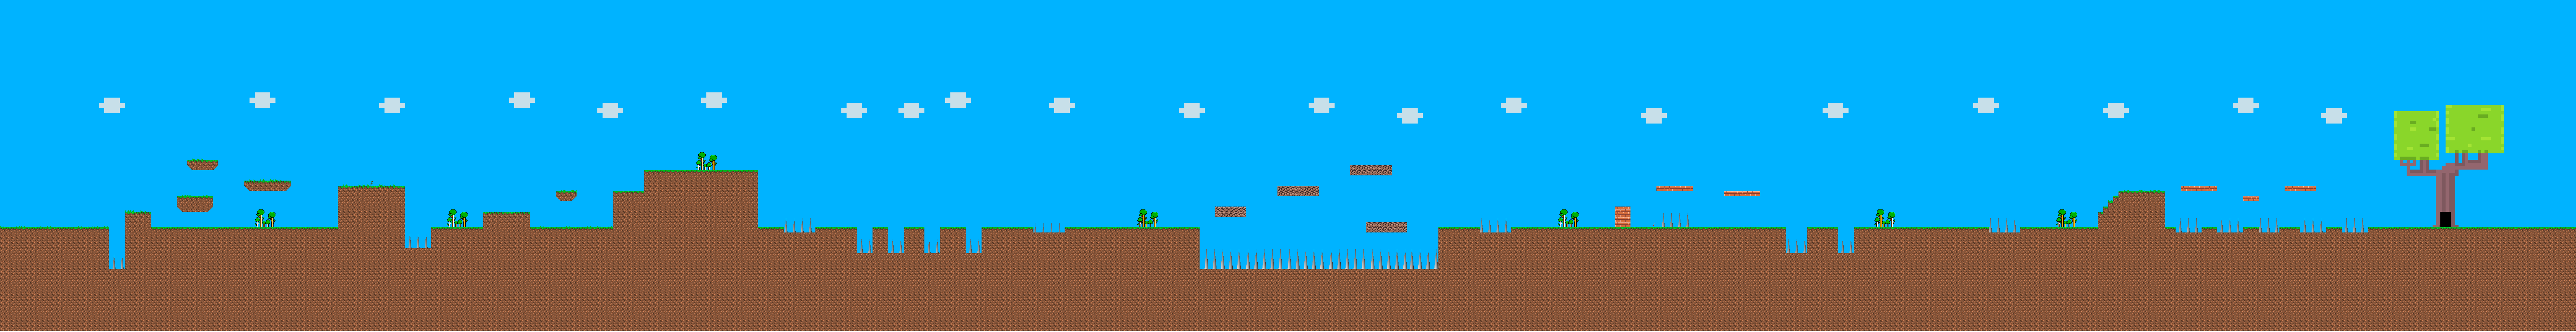
\includegraphics[width=1\textwidth]{Documentation/level_1.png}
 \caption{First level}
 \label{fig:FirstLevel}
\end{figure}

 \item The second level is inside the tree, where the player has to fight his way from bottom to the top of the tree to get to the eagle (boss) (see figure \ref{fig:SecondLevel}).

\begin{figure}[ht]
 \center
 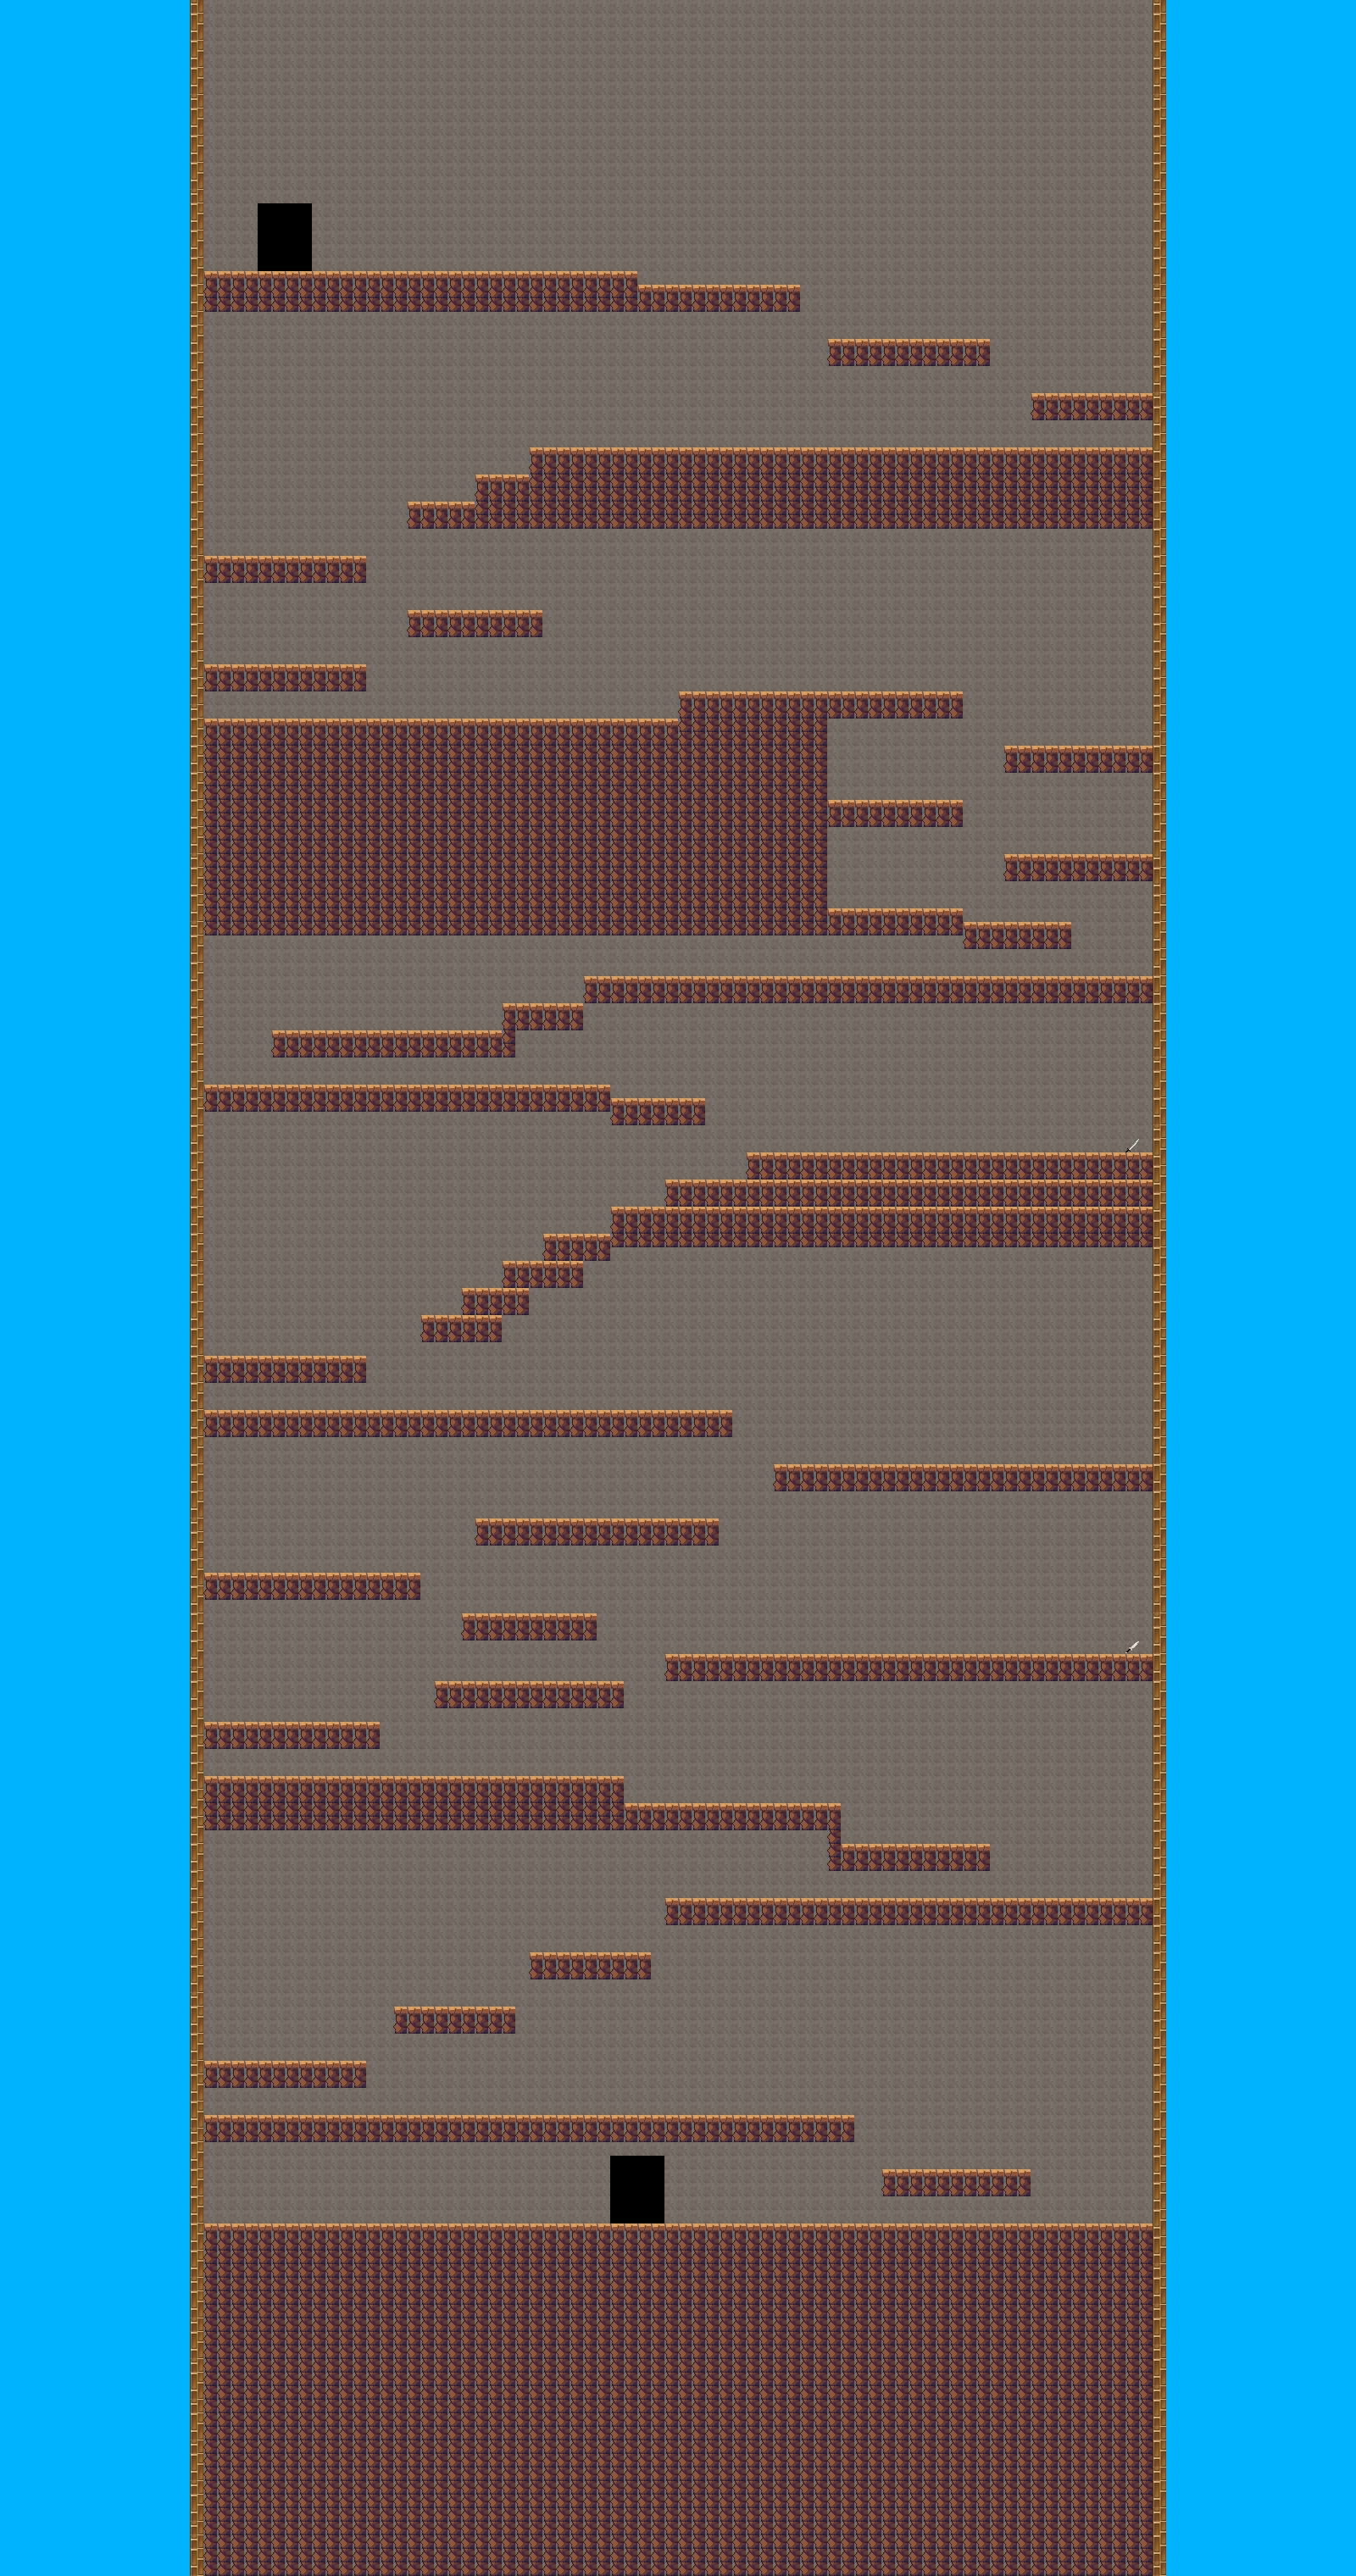
\includegraphics[width=0.4\textwidth]{Documentation/level_2.png}
  \caption{Second level}
 \label{fig:SecondLevel}
\end{figure}

 \item The last level is at the top of the tree where the player is encountered by an eagle that must be defeated to complete the game (see figure \ref{fig:BossLevel}).
 
 \begin{figure}[ht]
   \center
   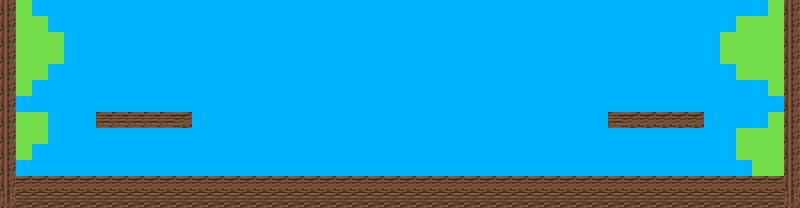
\includegraphics[width=0.9\textwidth]{Documentation/boss_level.png}
   \caption{Boss Level}
   \label{fig:BossLevel}
  \end{figure}
\end{itemize}

We created these maps by using a software called \texttt{Tiled}. Tiled is a map editor software, which is mostly used by developers to create maps \cite{TiledMapEditor}. Tiled is mostly used to make 8-bit styled based games, which is perfect for our game.

One of the reasons why we chose \emph{Tiled} as a map editor was that it's recommended by LibGDX itself in the documentation \cite{TileMaps}. Another reason was that the tutorial series for LibGDX on YouTube \cite{BrentAureliSuperMarioBros}, which we followed, had also used the Tiled map editor, which made very painless to follow. From our point of view working with the Tiled program was really easy to understand, since we managed to create a map with fairly easily with no experience whatsoever.

\subsection{Head-up display}

For the head-up display, we needed an icon for the remaining lives, the weapon strength and the Twitch effects (see section \ref{Twitch}). The health bar was trickier because it had to be resizable in the horizontal direction. The images in this section were all created with the image manipulation software GIMP \cite{GIMP}.

For the remaining lives, we used our own version of the iconic 8-bit heart (see figure \ref{fig:hud_heart_icon}). Thousands of those hearts can be found when googling "8-bit heart". The image size is 48 by 32 pixels, 16 extra pixels were added to the right side of the image to have a margin between the icon and the text in the game since it doesn't have a feature to do it itself. The icon can be seen in figure \ref{fig:hud_heart_icon}.

\begin{figure}[ht]
 \center
 
\includegraphics[width=0.1\textwidth]{Documentation/heart_icon.png}
 \caption{The remaining lives icon in the HUD}
 \label{fig:hud_heart_icon}
\end{figure}

The icon for the weapon strength is similar. It is also a 48 by 32-pixel image and based on already existing 8-bit art, but still created by ourselves completely (see figure \ref{fig:hud_weapon_strength_icon}). The icon shows a military knife with blood on its tip and around it, creating the illusion that it was just used. We think this is the clearest way to represent the strength of a weapon in an icon. The icon can be seen in figure \ref{fig:hud_weapon_strength_icon}

\begin{figure}[ht]
 \center
 
\includegraphics[width=0.1\textwidth]{Documentation/weapon_strength_icon.png}
 \caption{The weapon strength icon in the HUD}
 \label{fig:hud_weapon_strength_icon}
\end{figure}

The last of these icons simply shows the Twitch icon to represent the remaining time of an active effect that was given by Twitch chat (see section \ref{Twitch}). The icon has a 48 by 32-pixel resolution like the other icons and was self-drawn with the original logo as a template. The icon can be seen in figure \ref{fig:hud_twitch_icon}.

\begin{figure}[ht]
 \center
 
\includegraphics[width=0.1\textwidth]{Documentation/twitch.png}
 \caption{The Twitch icon in the HUD}
 \label{fig:hud_twitch_icon}
\end{figure}

The progress bars are a bit trickier because it has to be resizable in the horizontal direction to make it fit every screen size. LibGDX solves this scaling issue by using 9-Patch files \cite{NinePatchImage}. These images are normal PNG's, but with the extension \texttt{*.9.png}. Each nine-patch image has to be bigger by one pixel on each side of the image, which then contains black bars which describe the so-called \emph{patches}. A patch is simply the area of the image that is scalable, so the other graphical elements stay unaffected. IntelliJ has a built-in editor for nine patch images, which is a bit tricky to use but does the trick. When creating the skin for the HUD (see section \ref{DocHUD}), we needed to define a \texttt{knobBefore} image, which fills the progress bar. This image is simply one pixel wide and contains green pixels. The progress bar can be seen in figure \ref{fig:hud_health_bar}.

\begin{figure}[ht]
 \center
 
\includegraphics[width=0.75\textwidth]{Documentation/healthbar.png}
 \caption{The health bar in the HUD}
 \label{fig:hud_health_bar}
\end{figure}

The visuals of the health bar were inspired by the health bar of \emph{Stardew Valley} (see section \ref{StardewValley}). We adapted some of the main colors of their progress bar and also included a red cross on the left side of the progress bar. It is similar style-wise but created by ourselves completely and with our own ideas.

%------------------------------------------------

\subsection{Menus} \label{VisualDocMenus}

The navigational menus of the game were added as one of the last features. LibGDX provides a scene graph functionality with a few user interface widgets, but without any default style \cite{Scene2DUI}. Since the priority is functionality and not visuals, we used a community template called \emph{Flat Earth UI Skin} \cite{FlatEarthUISkin} to speed up the process of creating a working menu system.

The following figure \ref{fig:flat_earth_ui_skin} shows a template application, provided on the website, with all widgets to show the visuals of this template. Figure \ref{fig:main_menu_screenshot} then shows one of the menus that we created using this template.

\begin{figure}[ht]
 \center
 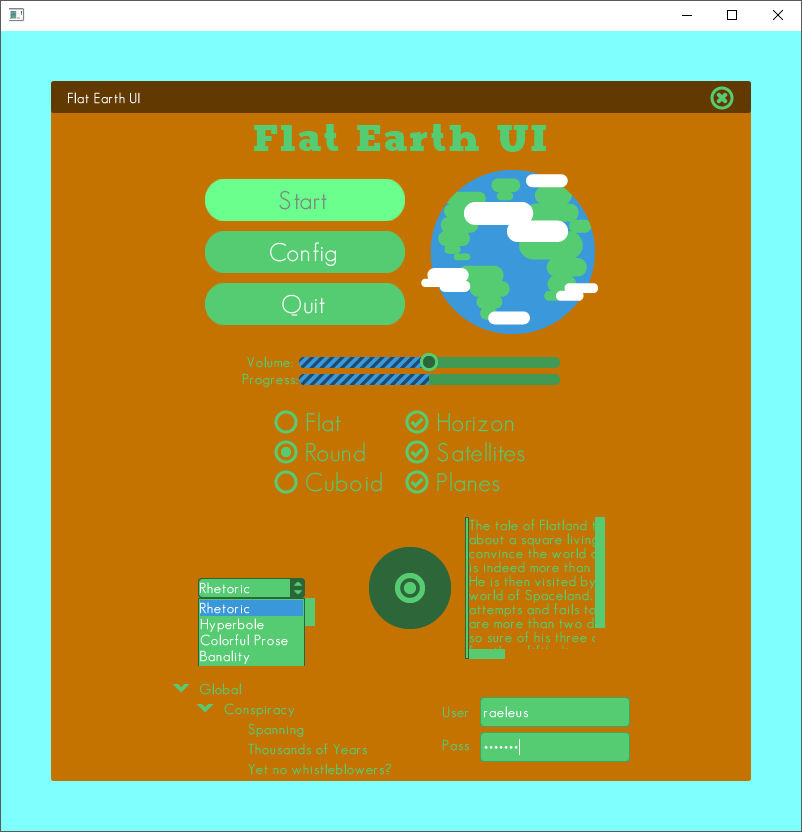
\includegraphics[width=0.75\textwidth]{Documentation/preview.png}
 \caption{Flat Earth UI Skin \cite{FlatEarthUISkin}}
 \label{fig:flat_earth_ui_skin}
\end{figure}

\begin{figure}[ht]
 \center
 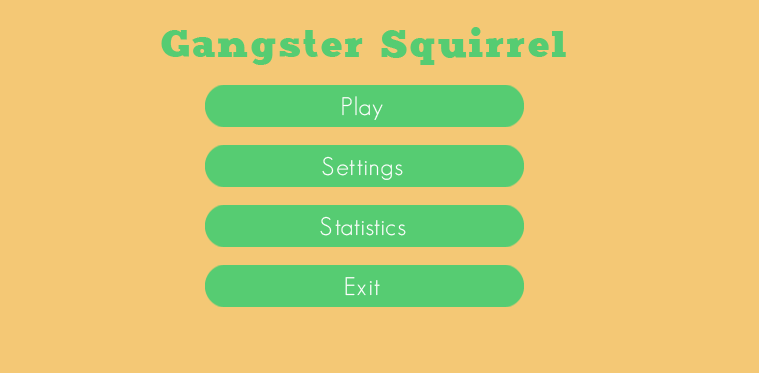
\includegraphics[width=0.75\textwidth]{Documentation/main_menu.png}
 \caption{The main menu}
 \label{fig:main_menu_screenshot}
\end{figure}

%------------------------------------------------

\clearpage
\section{Technical Documentation}

\subsection{Choosing the game engine} \label{DocGameEngine}

Deciding on a game engine is not an easy task, especially for Java. In the group, we split up the research of individual game engines, so that we can gather information about as many as possible before deciding on one. The procedure of finding relevant frameworks and game engines was fairly easy, by searching on a list of game engines on Wikipedia \cite{ListOfGameEngines}, using Google search and reading through forums to determine the public opinion on this topic. It quickly became apparent, that the market is rather thin when it comes to Java-based game engines, the big players like Unity \cite{UnityGameEngine} and Unreal Engine \cite{UnrealEngine} rely on \texttt{C} variations.

We researched the option of using a native Java library like \texttt{JavaFX} \cite{JavaFX} or Java AWT \cite{javaawt}, which would imply a lot of work on creating a core foundation for a game since it's not specifically made for this purpose. Most modern game engines come with certain standards, including an already existing application structure (with a game loop, scene management, events, and more). Popular engines usually also include their own or community made tools like map editors, asset managers, user interface composer, physics simulation, and so much more.

All of this would have the consequence of us having to code everything ourselves, limiting the outcome of the project due to the limited time. The group decided against this option by a majority vote. Not having to deal with a lot of very basic problems and therefore being able to develop the game farther and with more features, was more appealing to the majority of the group members.

Moving on, the group settled on a couple of game engines or frameworks to research: \texttt{libGDX} \cite{libGDX}, \texttt{LWJGL} \cite{LWJGL}, \texttt{jMonkeyEngine} \cite{jMonkeyEngine}, \texttt{mini2Dx} \cite{mini2Dx} and \texttt{Slick2D} \cite{Slick2D}. This selection is mostly by scavenging forum posts and the first page of Google for the search of "Java Game Engines". One particular \emph{Reddit} post \cite{RedditJavaGameEngines} named all of them.

Since \texttt{libGDX} is based on \texttt{LWJGL}, it is easy to compare them. \texttt{LWJGL} is very low-level and doesn't provide many features, compared to \texttt{libGDX}. It is also harder to start off with as a beginner in programming \cite{StackExchangeLibGDXLWJGL}, which is why we went with \texttt{libGDX}. Furthermore, the \texttt{jMonkeyEngine} is mainly developed for 3D applications, which rules it out for our project. 

\texttt{Mini2Dx} and \texttt{Slick2D} are both based on \texttt{LWJGL} too, but considerably smaller than \texttt{libGDX}. Comparing the GitHub pages of libGDX \cite{libgDXGitHub} and mini2Dx \cite{mini2DxGitHub}, this is quickly apparent. \texttt{LibGDX} has more than 400 contributors to the repository, while \texttt{mini2Dx} is only created and maintained by one person when looking at the contributors page. Meanwhile, \texttt{Slick2D} is hosted on BitBucket \cite{Slick2DBitBucket}, and hasn't even created a \emph{Read me} file. Judging from the documentation of the different game engines (can be found on the respective GitHub pages and for \texttt{Slick2D} on their own Wiki page \cite{Slick2DWiki}), it becomes even clearer, which engine is popular and which are not. \texttt{LibGDX} has a very extensive documentation with plenty of examples and in-depth explanations. \texttt{Mini2Dx} has a much smaller documentation, where most topics simply consist of a lot of pasted code without proper explanation. Meanwhile, \texttt{Slick2D}'s wiki page looks almost like an empty wiki template, because there is basically no documentation whatsoever.

This analysis is quite a clear statement, which choice would be the best and most painless way to go, so we decided to go with \texttt{libGDX}.

%------------------------------------------------

\newpage
\subsection{LibGDX Setup} \label{DocSetup}

To set up a libGDX project in IntelliJ IDEA, the official setup tool (see Figure \ref{fig:LibGDXSetupScreenshot}) needs to be used. This creates a Gradle project with all necessary files, adds optional extensions by default and defines the deployment platforms (Windows, macOS, Linux, Android, iOS, Blackberry, and HTML5). By clicking on \emph{Advanced} and selecting IntelliJ IDEA or a different IDE, this tool also creates the project files for the specific IDE.

\begin{figure}[ht]
 \centering
 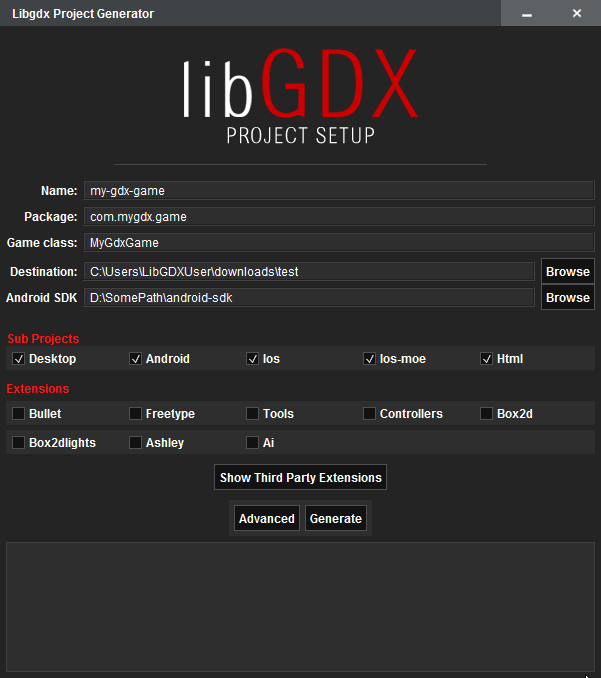
\includegraphics[width=0.8\textwidth]{libGDX_setup.png}
 \caption{libGDX Setup Tool}
 \label{fig:LibGDXSetupScreenshot}
\end{figure}

The import into IntelliJ is easy, just open the project and an import pop-up appears. By simply clicking \texttt{Ok}, everything will be imported and set up and the project is ready. To run the application in a desktop environment, the build configuration needs to be updated first, by setting the working directory to the \texttt{assets} folder of the project. With this being done, the set-up is complete.

%------------------------------------------------

\newpage
\subsection{Starting off}

Since no one in the group had any experience with LibGDX previously, we had to find a way to learn it and be able to set up a viable project structure. When searching for relevant tutorials online, we stumbled upon a YouTube playlist by Brent Aureli with tutorials on how to create a \emph{Super Mario Bros} \cite{SuperMarioBros} clone with LibGDX \cite{BrentAureliSuperMarioBros}.

The tutorial series helped us immensely in understanding how LibGDX works and how we had to set up and structure our game. This is mainly due to the nature of our game, which is similar to the original \emph{Super Mario Bros} in terms of gameplay. The playlist furthermore covers the creation of maps with the open source map editor \texttt{Tiled} (see section \ref{VisualDocMaps}) and the usage of the physics engine \texttt{Box2D} (see section \ref{DocCollisions}). The group reviewed about half of the playlist until we decided that we learned all basics that we need to create our own game.

However, it is important to note that we solely used this tutorial to learn about LibGDX and set up a basic 2D game. All code in the project is completely written by ourselves and we did not use any pre-made projects or classes from third parties.

%------------------------------------------------

\newpage
\subsection{The main class} \label{DocMainClass}

Since libGDX applications can run on multiple platforms (Windows, macOS, Linux, Android, iOS, Blackberry, and HTML5), the structure isn't as straightforward as a usual Java application. Considering the project delimitations (see section \ref{ProjectDelimitations}), this project is supposed to only run on the desktop platforms, which is why the focus is there.

Depending on the selected deployment platforms, the project will contain different kinds of \texttt{Launchers}, which handle the execution of the game. All desktop environments run on the same launcher since Java is cross-platform itself. The following code is all it takes to set it up, including setting certain configuration values, which are defined in the main class of the game.

\begin{minted}[linenos,breaklines]{java}
public class DesktopLauncher {
	public static void main (String[] arg) {
		LwjglApplicationConfiguration config = new LwjglApplicationConfiguration();

		config.title = MainGameClass.NAME;
		config.foregroundFPS = MainGameClass.FPS;
		config.width = MainGameClass.WIDTH;
		config.height = MainGameClass.HEIGHT;
		config.fullscreen = MainGameClass.FULLSCREEN;
		config.resizable = MainGameClass.RESIZABLE;

		new LwjglApplication(new MainGameClass(), config);
	}
}
\end{minted}

Going further, the actual code is located in the \texttt{core} directory of the project. Beside that, the generated \texttt{bytecode}, the \texttt{build gradle} file and the \texttt{assets} folder are located here. The assets folder contains all external files, like graphics, fonts and text files, which are used by the game.

The game starts off in the \texttt{MainGameClass}, which runs the very basic foundation of the game, by setting up important public static parameters like screen size, camera settings, gravity, and more. The main class extends libGDX's \emph{abstract} \texttt{Game} class, which itself implements the \texttt{ApplicationListener} \emph{interface}. LibGDX mostly works in an event-driven fashion, which is why there is no game loop \cite{libGDXLifeCycle}. The \texttt{render} method, however, can be considered as such, as it runs every frame. The flowchart in figure \ref{fig:LibGDXLifeCycle} explains the life cycle of a libGDX application.

\begin{figure}[ht]
 \center
 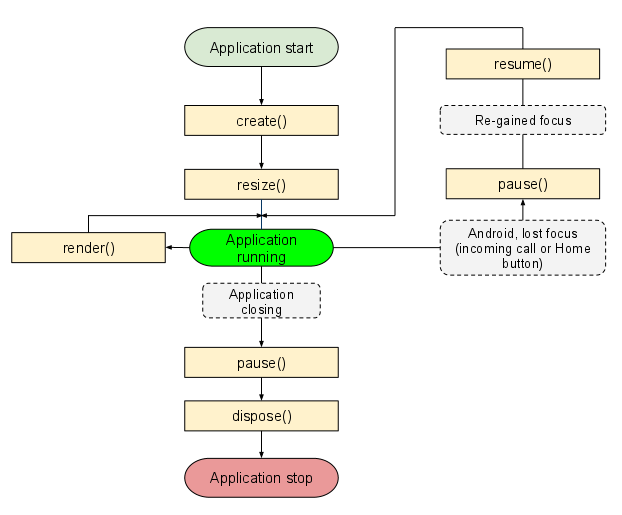
\includegraphics[width=1\textwidth]{Documentation/lifeCycle}
 \caption{LibGDX Life Cycle \cite{libGDXLifeCycle}}
 \label{fig:LibGDXLifeCycle}
\end{figure}

The main class has several purposes. It runs the main game cycle, sets up necessary parameters and has them publicly available to all classes, but also contains some important methods, like resetting certain values in the save files (player lives, current time) and also methods to exit the application. The following code shows the two overloaded exit methods. The difference is simply, that one of them prints out a message before exiting, while the other does not.

\begin{minted}[linenos,breaklines]{java}
public void exitApplication() {
	resetTimer();
	resetPlayerLifes();
	Gdx.app.exit();
	System.exit(0);
}

public void exitApplication(String errorMessage) {
	if (errorMessage != null && !errorMessage.isEmpty()) {
		System.err.println(errorMessage);
	}

	exitApplication();
}
\end{minted}

The methods \texttt{resetTimer()} and \texttt{resetPlayerLifes()} reset the values for the current game time and the current lives of the player in the JSON save files, because they are being used by the game and need to be temporary, or the lives or the time will not start from the default value, when starting the game the next time. These values need to be stored in a file, because the entire play screen class is being reloaded, when the player respawns, and therefore resetting all run time variables (see section \ref{DocJSONfiles}).

The game is then being closed by calling the libGDX method \texttt{Gdx.app.exit()}, which disposes of all disposable resources in the application and close the game. This works just fine, but usually prints out a bunch of irrelevant errors, which can be more or less suppressed by calling the native Java method \texttt{System.exit()}. The error code \texttt{0} means the execution went just fine with no errors.

When the main class is done setting things up, including the creation of a new Thread for a connectivity with Twitch (see documentation at \ref{Twitch}), the game switches the \texttt{Screen} to the \texttt{SplashScreen} class, which simply displays a splash screen and then switches to the \texttt{PlayScreen} class, which is the main screen of the game, containing the actual gameplay and manages, how it all comes together. It implements libGDX's \texttt{Screen} class and follows a similar life cycle as described for the main game class. The documentation for this class can be found in section \ref{DocPlayScreen}.

%------------------------------------------------

\newpage
\subsection{The application structure} \label{DocApplicationStructure}

As described in the previous section, the \texttt{MainGameClass} is the entry point of the application, followed by the most important class of the game, the \texttt{PlayScreen}. This does not nearly describe the structure of the entire project though since there are dozens of classes in the project.

The following figure \ref{fig:minClassDiagram} is a minimised version of the class diagram of the project, which is supposed to show the relation between classes and the overall structure. A flowchart of the game can be found in section \ref{DocMenus}.

\begin{figure}[ht]
 \centering
 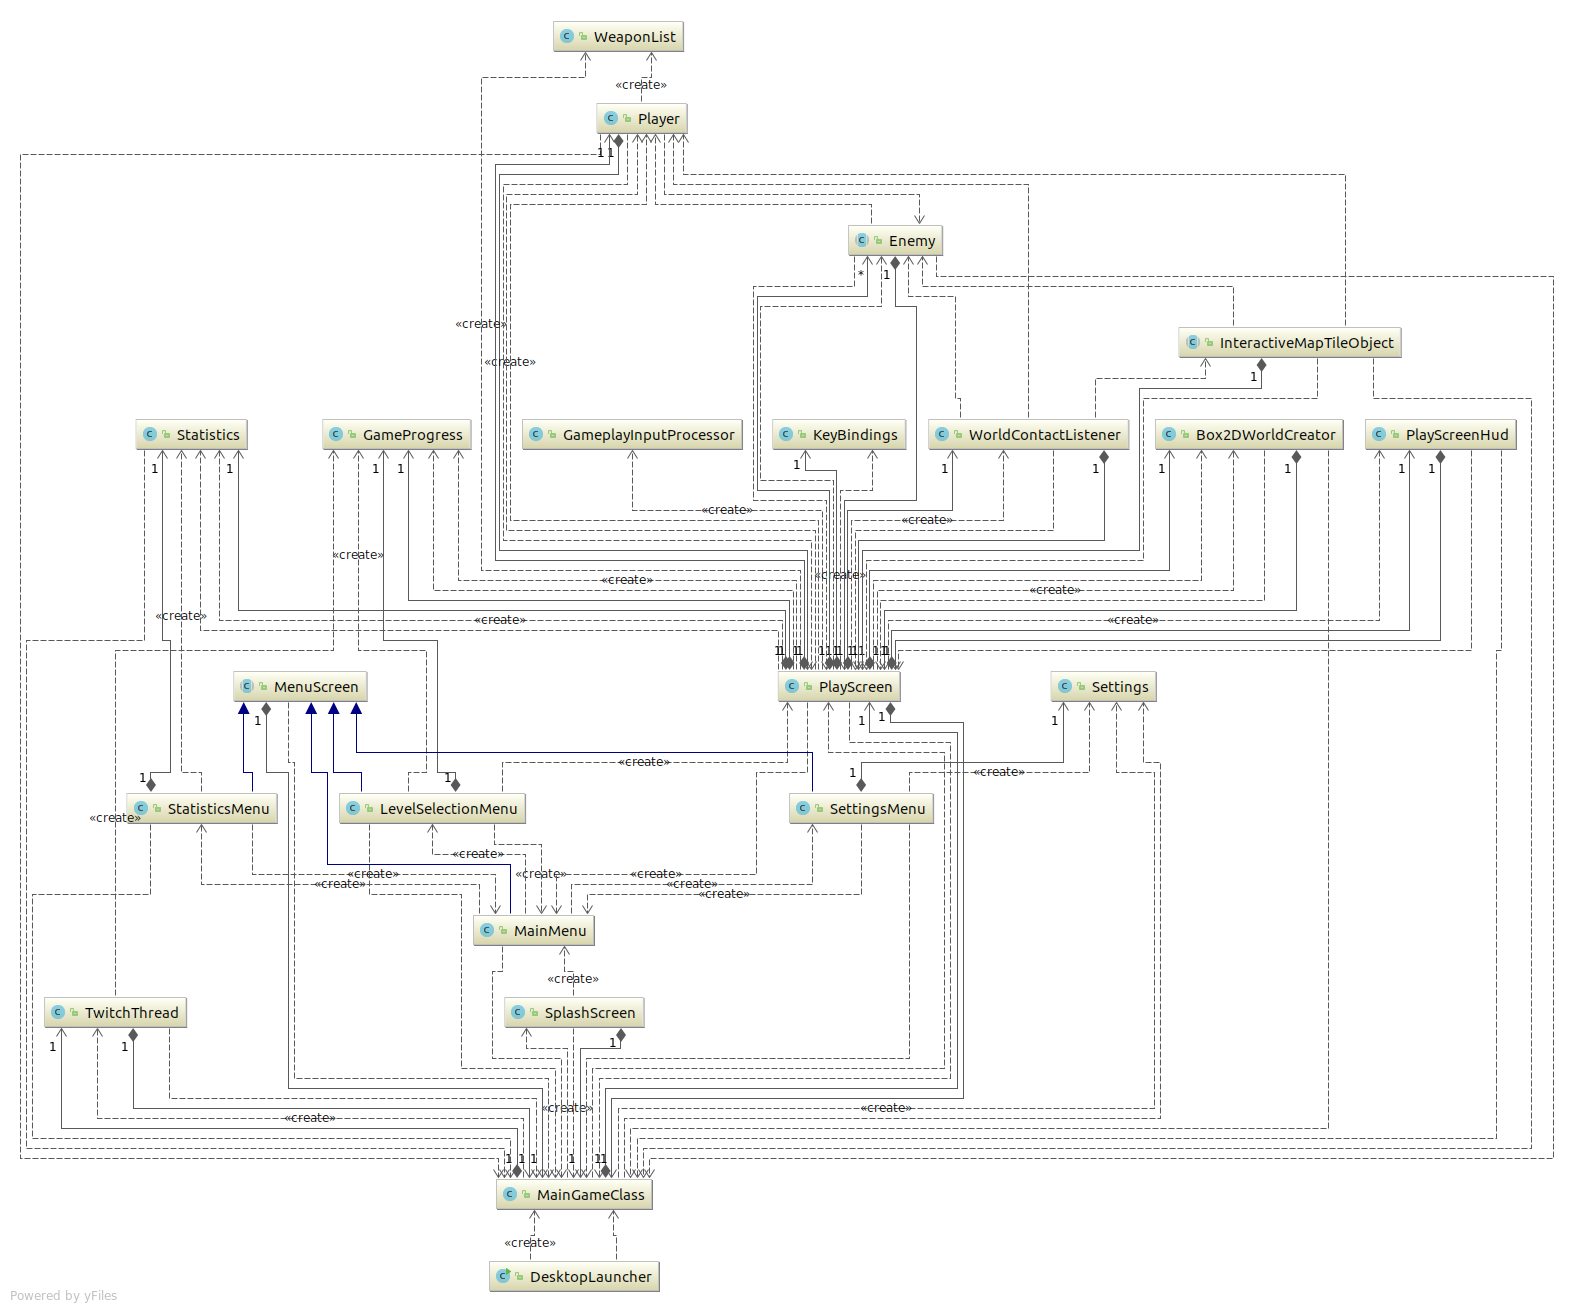
\includegraphics[width=1\textwidth]{Documentation/class_diagram_minimized.png}
 \caption{Minimised class diagram}
 \label{fig:minClassDiagram}
\end{figure}

The application starts with the \texttt{DesktopLauncher}. Other platforms have different launchers, but this project is only available on desktop platforms and is, therefore, the only launcher. The full diagram also shows a \texttt{HtmlLauncher} for running it in a web browser, which is not used, nor supported in our case. We simply checked the box for it in the set up of the project and didn't remove it.

The first actual class of the game is the \texttt{MainGameClass}, which was already explained in the previous section. From there, a separate thread for the Twitch integration is created (see section \ref{Twitch}). The reason, why so many dotted arrows point back to the main class, is because of all the public parameters that are stored here and needed by many classes.

Following that, the main game class creates the \texttt{SplashScreen}, which just shows an image for a few seconds and then switches to the \texttt{PlayScreen}. In here, everything gameplay relevant is being created and handled (see section \ref{DocPlayScreen}). 

The following list briefly describes each class that can be seen in the minimised class diagram, except the ones already described. Many of these classes have subclasses or associated classes, which are not relevant for the structure but can be seen in the full diagram (see section \ref{AppendixClassDiagramFull}).

\begin{itemize}
 \item \textbf{Box2DWorldCreator}: responsible for creating the physics environment of the map (see section \ref{DocMaps})
 \item \textbf{WorldContactListener}: detects and handles all collision between physics objects (see section \ref{DocCollisionDetection})
 \item \textbf{InteractiveMapTileObject}: an abstract class for static map objects, includes physical body set up and collision handling (see section \ref{DocPhysicsAndBodySetup})
 \item \textbf{Enemy}: an abstract class for different enemy objects, includes physical body set up, collision handling and enemy movement (see section \ref{DocEnemyClass})
 \item \textbf{Player}: the definition of the player as physical entity and as texture. Everything from player animations, moving, attacking and switching weapons is done here (see section \ref{DocPlayerClass})
 \item \textbf{PlayScreenHud}: sets up and manages the "Head-Up Display", containing items like the health bar and the timer (see section \ref{DocHUD})
 \item \textbf{GameplayInputProcessor}: registers key press events and handles them appropriately (see section \ref{DocKeyBindings})
 \item \textbf{KeyBindings}: reads and writes associated keys with certain actions to a file (see section \ref{DocKeyBindings})
 \item \textbf{GameProgress}: reads and writes the user's progress in the game to a file (see section \ref{DocJSONfiles})
 \item \textbf{Statistics}: reads and writes the user's statistics to a file (see section \ref{DocJSONfiles})
 \item \textbf{WeaponList}: reads and writes all available weapons in the game to a file (see section \ref{DocJSONfiles})
 \item \textbf{Settings}: reads and writes the game settings to a file (see section \ref{DocJSONfiles})
 \item \textbf{MenuScreen}: an abstract class that provides a basic functionality to set up menu screens (see section \ref{DocMenus})
 \item \textbf{MainMenu}: the entrance of the game, the user can select to play, change settings and view statistics or exit the application
 \item \textbf{LevelSelectionMenu}: a menu to select which level the user wants to play
 \item \textbf{StatisticsMenu}: a menu to view and reset all statistics
 \item \textbf{SettingsMenu}: a menu to change the game settings
\end{itemize}

A flowchart of the navigation within the game can be found in the documentation of the menus (see section \ref{DocMenus}).

%------------------------------------------------
 
 \newpage
\subsection{The play screen} \label{DocPlayScreen}

The \texttt{PlayScreen} combines all elements of the project into a playable environment. It is by far the longest class in the project and contains the most relevant and crucial logic to run the game.

Since this class implements libGDX's \texttt{Screen} interface, it follows the same lifecycle that was previously described in section \ref{DocMainClass} and can be seen as a flowchart in figure \ref{fig:LibGDXLifeCycle}. 

This section is divided into several subsections to explain each part of the class.
 
\subsubsection{Constructor and set-up}

In the constructor, everything that has to be set up before the actual gameplay starts will be done here. The constructor takes in an instance of the main game class, with which you can control the entire game logic. It is assigned to a local variable of its type and is available through a getter in the \texttt{PlayScreen}. With this, every class that needs to have access to the main game class or play screen will simply be given the play screen as a parameter and through this, the main game class is also available.

The constructor then calls the method \texttt{setupScreen()}, which handles the rest of the set-up. Everything can obviously just be written inside the constructor, but an external method is a cleaner way of doing it.

In there, the textures will be loaded into instances of the class \texttt{TextureAtlas}, the camera and viewport are created, the map is loaded, collision boxes are set up, the player and enemies are spawned, key bindings are loaded, input listeners are assigned, sounds and music are loaded, and the gameplay timer is initialized.

As an example of the many things that are done here, we can take a look at how the player is set up. The set up of the textures, animations and physics is already covered in the \texttt{Player} class documentation (see section \ref{DocPlayerClass}), but the \texttt{PlayScreen} defines a few more important things.

The following code snippet is taken from the \texttt{setupPlayer()} method.

\begin{minted}[linenos,breaklines]{java}
switch (gameProgress.getCurrentLevel()) {
  case 1:
    player = new Player(this, level_1_spawnPositionX, level_1_spawnPositionY);
    break;
  // Omitted case 2 & 3 to save space ...
  default:
    game.exitApplication("No current level defined, exiting application");
    break;
}

setUpPlayer();
\end{minted}

The current level is retrieved from a \texttt{GameProgress} object, which is a class that maintains a \texttt{JSON} file that stores basic information about the player's progress. More information on this can be found in the documentation for \texttt{JSON} files in section \ref{DocJSONfiles}.

Based on that information, the logic assigns the local \texttt{Player} variable a new instance of the \texttt{Player} class and gives it the instance of the \texttt{PlayScreen} class, as described in the introduction of this section, accompanied with the desired spawn coordinates. These coordinates are field variables of the type \texttt{Integer} and give a position in tiles, counting from zero and starting in the lower left corner of the map. The \texttt{Player} class will then convert these values into real coordinates by multiplying them by the tile pixel size and then spawn the Player at that position.

If the current level is not in the case list, which it will never be under normal circumstances, the game is closed by using the overloaded \texttt{exit()} method that was mentioned in section \ref{DocMainClass}.

After this, the method \texttt{setUpPlayer()} method is called, which takes care of the rest and looks like this:

\begin{minted}[linenos,breaklines]{java}
private void setUpPlayer() {
  // Player health
  player.setHealth(gameProgress.getPlayerMaxHealth());

  // Add default weapon, if the players weapon list is empty
  if (gameProgress.getPlayerWeaponList().size() == 0) {
    ArrayList<WeaponObject> playerWeaponList = gameProgress.getPlayerWeaponList();
    playerWeaponList.add(allWeapons.get(0));
    gameProgress.setPlayerWeaponList(playerWeaponList);
  } else if (gameProgress.getPlayerWeaponList().size() > 0) {
    player.setWeapons(gameProgress.getPlayerWeaponList());
  }

  // Movement variables
  player.setJumpImpulseVelocity(gameProgress.getPlayerJumpImpulseVelocity());
  player.setWalkImpulseVelocity(gameProgress.getPlayerWalkImpulseVelocity());
  player.setClimbImpulseVelocity(gameProgress.getPlayerClimbImpulseVelocity());
  player.setMaxWalkVelocity(gameProgress.getPlayerMaxWalkVelocity());
  player.setMaxClimbVelocity(gameProgress.getPlayerMaxClimbVelocity());
}
\end{minted}

As of first, the field variable \texttt{health} is set to the maximum at the beginning of each level, which is stored in the \texttt{gameprogress.json} file, in case we want to implement upgrades to the player, which may increase the player's maximum health. The entire system is mainly designed for scalability, so it is easy to implement features at a later point in time.

The next thing is to check, if the player has any weapons in his inventory. The equipped weapons are also stored in the \texttt{gameprogress.json} file. If the inventory is empty, which is only the case if the file is empty or deleted, the default weapon will be added by getting the first weapon in the list of all available weapons in the game, which is stored in the \texttt{weaponlist.json} file. The variable \texttt{allWeapons} is an \texttt{ArrayList} of the type \texttt{WeaponObject}, which is initialized in the field of the class, containing all weapon objects in the game.

The last thing here is to assign the variables that are used for moving the player. They are also stored in the \texttt{gameprogress.json} file for scalability, in case we want to change the values with level-ups or similar mechanics. The values are assigned to field variables of the \texttt{Player} class, which are later read by the \texttt{PlayScreen} again, when handling input actions and applying impulses (making it move) to the player's body. These values can obviously just be read from the file, when they are needed, but we wanted to keep the structure as clear as possible and wanted to keep all player related variables in the player's class.

\subsubsection{The render method}

The abstract \texttt{render} method is called each frame and takes care of drawing the next frame, simulating the next step in the physics simulation, handling input, and more.

Since this method is the largest part of the class, we divided it into several methods that are linked to each other. The \texttt{render} method directly calls the \texttt{update} method, which itself directly calls the \texttt{handleInput} method. This means, that the user input is handled first, then all objects in the game are updated (this includes objects like the game timer, physics simulation, head-up display, camera, ...). The \texttt{update} method itself calls the two methods \texttt{updateCamera} and \texttt{destroyQueuedBodies}. The first of both updates the camera position relative to the player's position using an interpolation value. The second method handles the destruction of unwanted bodies in the physics simulation. A detailed explanation of this can be found in section \ref{DocDestroyingBodies}.

The \texttt{handleInput} method contains all code to check for user input. An example would be the jump mechanics:

\begin{minted}[linenos,breaklines]{java}
if (isPressingJump && player.getIsOnJumpableGround() && player.body.getLinearVelocity().y == 0) {

  player.body.applyLinearImpulse(new Vector2(0, player.getJumpImpulseVelocity()), player.body.getWorldCenter(), true);

  if (MainGameClass.PLAY_SOUNDS) {
    jumpSound.play();
  }

  statistics.setJumpsMade(statistics.getJumpsMade() + 1);
}
\end{minted}

In the documentation of the key bindings (see section \ref{DocKeyBindings}), we explained how we store key bindings in a JSON file and then read them into a list of Integers. When one of the assigned keys is pressed, the boolean \texttt{isPressingJump} is toggled and this is how we can determine if one of the jump keys is being pressed.

Moreover, the player has to be on the ground to be able to jump. In the beginning, we had the bug that the player could stick to a ceiling when holding down a jump button, and also double jump when mid-air, because we only checked for the vertical velocity, and if it was zero, we allowed the jump. We solved this by creating an extra object layer in the maps, which were simply lines on the surface. When the player is in contact with one of these objects, we allowed the jump. When colliding with such an object, the field variable \texttt{isOnJumpableGround} of the \texttt{Player} class is toggled.

Finally, when the vertical velocity is also zero, we allow the player to jump. This is done by applying an impulse in the positive vertical direction to the body of the player. After that, a jump sound is played and the jump statistic is increased by one (see section \ref{DocJSONfiles}).

In the \texttt{update} method, all time, physics and camera related are updated. For example, the timer is maintained by this code:

\begin{minted}[linenos,breaklines]{java}
deltaTimeCount += deltaTime;
if (deltaTimeCount >= 1) {
  timer++;
  deltaTimeCount = 0f;
}
\end{minted}

The floating point timer, \texttt{deltaTimeCount}, sums the delta times of each frame together until it reaches a full second. The delta time is the real time between the last frame and the current frame in seconds. When a full second is reached, the delta timer counter is set back to zero and the real game timer, which is an \texttt{integer}, will be increased by one second.

When the input handling and updating is finally done, the real rendering happens. As of first, the previous frame has to be "deleted" or the next frame will draw on top of it otherwise, creating a visual mess. This is done with two lines of \texttt{OpenGL} code:

\begin{minted}[linenos,breaklines]{java}
Gdx.gl.glClearColor(0, 0, 0, 1);
Gdx.gl.glClear(GL20.GL_COLOR_BUFFER_BIT);
\end{minted}

After this is done, several \texttt{render} methods of different kinds are called. For example, the player, all enemies, the HUD, the world renderer all have their own render method that needs to be called from here.

\subsubsection{Respawning and finishing a level}

The \texttt{PlayScreen} class has a few more important methods besides the set-up of the screen and updating it. This includes two methods used for respawning the player when he dies and finishing a level. The method to finish a level is linked to the respawn method, which is why they are both in one section.

When the player collides with an object that is marked as a "Finish", the game needs to save the progress and load the next level. The first thing is to save the timer to the statistics file, if the player set a new high score (see section \ref{DocJSONfiles}). The following code snippet from the \texttt{levelFinished} method investigates this.

\begin{minted}[linenos,breaklines]{java}
if (statistics.getHighscoreTimes()[gameProgress.getCurrentLevel() - 1] > 0) {
  if (timer < statistics.getHighscoreTimes()[gameProgress.getCurrentLevel() - 1]) {
    long[] tmp = statistics.getHighscoreTimes();
    tmp[gameProgress.getCurrentLevel() - 1] = timer;
    statistics.setHighscoreTimes(tmp);
  }
} else {
  long[] tmp = statistics.getHighscoreTimes();
  tmp[gameProgress.getCurrentLevel() - 1] = timer;
  statistics.setHighscoreTimes(tmp);
}
\end{minted}

The highscores are stored in an array of the type \texttt{long} within the \texttt{statistics} JSON file, with one value for each level. This array is retrieved in the first if-statement and the relevant item for the current level is checked, if it above zero. If this is not the case, this means that no highscore has been set yet, because the initial value of each item is zero since \texttt{long} is a primitve data type. 

If there is no highscore for the current level yet, the current timer is written to a temporary copy of the highscores array at the relevant position. The new and updated highscore array is then written to the file.

However, if there is already a highscore for the current level, the current game time is compared with the previous record and if the new time is better, it will also be saved to the file as a new highscore.

Going further, the current level is stored in the \texttt{gameprogress} JSON file and is used to determine which level needs to be loaded, when setting up the play screen. When a level is finished, this obviously needs to be updated. The following code snippet does exactly that.

\begin{minted}[linenos,breaklines]{java}
if (gameProgress.getCurrentLevel() < MainGameClass.NUMBER_OF_LEVELS) {
  gameProgress.setCurrentLevel(gameProgress.getCurrentLevel() + 1);
} else {
  log("Game finished, no more levels to play");
}
\end{minted}

If the current level is not the last one, the number is simply bumped up by one. The total amount of levels is stored in a public field variable of the \texttt{MainGameClass}.

Ignoring a few minor statistics modifications, the \texttt{respawnPlayer} methody is finally called from here, which reloads the entire play screen.

In this method, more statistics are saved and timers reset. After all of this is done, the following line of code reloads the play screen and starts a new level from scratch.

\begin{minted}[linenos,breaklines]{java}
game.setScreen(new PlayScreen(game));
\end{minted}

\subsubsection{Spawning enemies} 

To make life as easy as possible, we added a spawn method for enemies that only requires an enemy type and the desired spawn position. When reading this information from the map, this method can be called and reduces duplicated code.

\begin{minted}[linenos,breaklines]{java}
public void spawnEnemy(Class<? extends Enemy> type, int spawnPositionX, int spawnPositionY) {
  if (type == FrogEnemy.class) {
    enemies.add(new FrogEnemy(this, spawnPositionX, spawnPositionY));
  } else if (type == MonkeyEnemy.class) {
    enemies.add(new MonkeyEnemy(this, spawnPositionX, spawnPositionY));
  }
}
\end{minted}

The method takes a parameter of the type \texttt{Class}, which can be any type but has to extend the \texttt{Enemy} class. This means, only enemies are accepted as a type. The other two parameters are the tile positions of the desired spawn point, counting from zero at the lower left corner of the map.

Depending on the type of enemy, the list of all enemies in the level gets a new instance of this enemy, which automatically spawns it on the map. The tile positions are then converted to actual pixel coordinates by the constructor of the enemy class.

%------------------------------------------------
 
\newpage
\subsection{Physics and collision detection} \label{DocCollisions}

One of the most important aspects of a game is certainly the collision detection and handling between objects. Without it, it would not be possible to even make the player walk on a flat surface.

LibGDX utilizes \texttt{Box2D}, a well known physics engine for rigid body simulations, originally written in \texttt{C++} and since ported into many other languages. It was used in several well known games like \emph{Angry Birds}, \emph{Tiny Wings}, \emph{Limbo}, and \emph{Happy Wheels} \cite{box2DGithub}\cite{box2DWikipedia}.

\subsubsection{Physics and map objects setup} \label{DocPhysicsAndBodySetup}

As described in the map documentation (see section \ref{DocMaps}), the maps that are created in the \texttt{Tiled} map editor, can contain so-called object layers, which contain information about shapes, that will be used as collision shapes in the game. For example, when creating a simple two-dimensional map in a map editor, you obviously add graphics. The game can't know, what the world actually looks like just by the textures though. It needs concrete information on what to treat as walkable ground, what enemies are, where a finish line might be, and so on. This is where the object layers come into play.

Before we can go on to detecting collisions and handling them, we first need to create a world and all it's bodies, in order to play with them. The first step towards this is done in the \texttt{PlayScreen} class within the constructor. Here, a \texttt{World} object is created, which contains all bodies and controls the entire physics simulation. The following line of code initializes the world, with the parameter of the gravity, which is roughly $9.81m/s^2$ in the negative direction of the Y-axis. This value is a final floating point value, defined in the main game class amongst the other constant values. The second parameter, \texttt{doSleep}, improves the performance of the simulation if set to \texttt{true}, by not simulating inactive bodies, which means bodies that do not move or interact in any other way with the world, at the specific time.

\mint{java}{world = new World(new Vector2(0, - MainGameClass.GRAVITY), true);}

Furthermore, a \texttt{Box2DWorldCreator} and \texttt{WorldContactListener} class are initialized in the same constructor. Both of them are custom written classes, the first one being responsible for reading the shapes from the map file and translating them into actual bodies in the world. This is partially described in the maps documentation in section \ref{DocMaps}. The second class implements libGDX's \texttt{ContactListener} class and constantly listens for collisions between objects and calls the required methods. This is documented in the next section (\ref{DocCollisionDetection}).

All static objects in the map are child objects of the abstract \texttt{InteractiveMapTileObject} class, which defines a standard structure for these objects. Since all objects in the map have a rectangular shape, this abstract class implements a standardized way of setting up the body of each object. All it needs to know is the rectangle, which defines shape and position of the object, and if it is a sensor. If an object is a sensor, collisions will be detected as usual, but other objects can't collide with it visually and will simply move through them. This can be useful for many different purposes, for example, the weapon pick-up mechanics.

As an example, we take the \texttt{DeathTile} class and follow it's steps to creation. This type of object has the purpose of killing both players and enemies if they come in contact with it. This will often be graphically represented by spikes. As described in section \ref{DocMaps}, for each object in an object layer, the program creates an instance of the related child class of an \texttt{InteractiveMapTileObject}. In this case, a \texttt{DeathTile}. The object will then be added to a list, which contains all objects of this type.

\mint{java}{deathTileObjects.add(new DeathTile(screen, rectangle));}

The constructor demands the \texttt{PlayScreen} object as the first parameter, so it has access to it. The second parameter is the rectangle that was read from the map file.

The following code snippet is from the \texttt{DeathTile} class in order to explain the creation of such objects.

\begin{minted}[linenos,breaklines]{java}
public class DeathTile extends InteractiveMapTileObject {

  private PlayScreen playScreen;

  public DeathTile(PlayScreen screen, Rectangle bounds) {
    super(screen, bounds, true);
    this.playScreen = screen;

    fixture.setUserData(this);
    createFilterMask();
  }

  @Override
  public void onPlayerBeginContact(Player player) {
    playScreen.setPlayerCurrentHealth(-1);
  }

  @Override
  public void onPlayerEndContact(Player player) { }

  @Override
  public void onEnemyBeginContact(Enemy enemy) {
    enemy.setHealth(-1);
  }

  @Override
  public void onEnemyEndContact(Enemy enemy) { }

  @Override
  public void createFilterMask() {
    Filter filter = new Filter();
    filter.categoryBits = MainGameClass.CATEGORY_DEATHTILE;
    filter.maskBits = MainGameClass.MASK_DEATHTILE;
    fixture.setFilterData(filter);
  }
}
\end{minted}

In the constructor, the \texttt{super} method is called, which is the constructor of the InteractiveMapTileObject, which handles the physics setup. In addition to the \texttt{PlayScreen} and the rectangle, a boolean variable is passed as a parameter. It defines, if the object is a sensor, as described above.

Still in the constructor, the \texttt{User Data} of the \texttt{fixture} is set to the class itself, \texttt{this}. The \texttt{fixture} is a \texttt{protected} variable of the parent class and therefore available in the child class scope. The \texttt{User Data} is a value that is important for collision detection. It can be any \texttt{Object} and will later be used to identify a collided object, as described in section \ref{DocCollisionDetection}.

The method \texttt{createFilterMask} is an abstract method of the parent class, that each child has to implement. It sets up collision filtering, which is also described in section \ref{DocCollisionDetection}.

The four remaining abstract methods are always called, when either a player or enemy is colliding with this specific \texttt{DeathTile} object. In this case, when a contact begins, the health of either of those will be set to $-1$, which kills them in the next frame.

The last code snippet for this section finally shows, how a map object is actually created. The code is from the \texttt{InteractiveMapTileObject} class. Besides the shown constructor, the class defines the five abstract methods and contains two methods that are used for picking up weapons (see section \ref{DocWeaponCollection}).

\begin{minted}[linenos,breaklines]{java}
public InteractiveMapTileObject(PlayScreen screen, Rectangle bounds, boolean isSensor) {
    this.playScreen = screen;
    this.world = screen.getWorld();
    this.map = screen.getMap();
    this.bounds = bounds;

    BodyDef bodyDef = new BodyDef();
    FixtureDef fixtureDef = new FixtureDef();
    PolygonShape shape = new PolygonShape();

    bodyDef.type = BodyDef.BodyType.StaticBody;
    bodyDef.position.set((bounds.getX() + bounds.getWidth() / 2) / MainGameClass.PPM, (bounds.getY() + bounds.getHeight() / 2) / MainGameClass.PPM);
    body = world.createBody(bodyDef);

    shape.setAsBox(bounds.getWidth() / 2 / MainGameClass.PPM, bounds.getHeight() / 2 / MainGameClass.PPM);
    fixtureDef.shape = shape;
    fixtureDef.isSensor = isSensor;
    fixture = body.createFixture(fixtureDef);
  }
\end{minted}

In here, the body of the map object is defined with the help of a \texttt{body definition}, \texttt{fixture definition} and \texttt{polygon shape}. The type of the body is \texttt{static} since the map objects should not move upon contact with another object like the player and enemies do (they are \texttt{dynamic}). The position of the body is then being set to the middle of the rectangle. \texttt{bounds.getX()} and \texttt{bounds.getY()} return the lower left corner of the object, which is why half of the width and height is added. This value is then being divided by the \texttt{pixels per meter} scaling unit, which \texttt{Box2D} needs since it's never a good idea to code in pixels. A clarification can be found in a great Stackoverflow answer \cite{stackoverflowPPM}. The shape is then set to a box, with the width and height of the rectangle. The values are divided into two because the \texttt{setAsBox} method takes in the radius of a box.

%------------------------------------------------

\subsubsection{Stepping the simulation} \label{DocSteppingTheSimulation}

The physics simulation has to be updated each frame, which is why the following line of code is called each frame in the \texttt{update} method (originally the \texttt{render} method) of the \texttt{PlayScreen}.

\mint{java}{world.step(1 / (float) MainGameClass.FPS, 6, 2);}

The first parameter is the time that the world is supposed to simulate The game uses a fixed FPS (frames per second) value to make gameplay consistent on all devices. The second and third parameter are the velocity and position iterations. This defines how often the velocity and position are calculated. This means, the higher the value, the more precise is the simulation. $6$ and $2$ are the recommended values by libGDX \cite{stepValues}.

%------------------------------------------------

\subsubsection{Collision detection} \label{DocCollisionDetection}

In order to detect and handle collisions, libGDX provides a \texttt{ContactListener} interface, that we can use to process all collisions in the world. It is event-driven, which means the methods \texttt{beginContact} and \texttt{endContact} will only be triggered, when a collision happens, not each frame. You then get a \texttt{Contact} object, which manages two colliding shapes and gives the program information about them.

The contact listener is simply attached to the \texttt{Box2D} world in the \texttt{PlayScreen}:

\begin{minted}[linenos,breaklines]{java}
worldContactListener = new WorldContactListener(this);
world.setContactListener(worldContactListener);
\end{minted}

The following code snippet is from the \texttt{WorldContactListener} class and shows the collision handling for player contacts. The code for enemy collisions is very similar and can be found in the source code. To keep it short, the collision between player and enemies is also cut out.

\begin{minted}[linenos,breaklines]{java}
private void processContact(Contact contact, boolean beginOrEndContact) {

    Fixture fixtureA = contact.getFixtureA();
    Fixture fixtureB = contact.getFixtureB();

    if (fixtureA.getUserData() instanceof Player || fixtureB.getUserData() instanceof Player) {
      Fixture player = fixtureA.getUserData() instanceof Player ? fixtureA : fixtureB;
      Fixture collidedObject = player == fixtureA ? fixtureB : fixtureA;

      if (collidedObject.getUserData() instanceof InteractiveMapTileObject) {
        if (beginOrEndContact) {
          ((InteractiveMapTileObject) collidedObject.getUserData()).onPlayerBeginContact((Player) player.getUserData());
        } else {
          ((InteractiveMapTileObject) collidedObject.getUserData()).onPlayerEndContact((Player) player.getUserData());
        }
      }
    }
  }
\end{minted}

The method \texttt{processContact} is called from \texttt{beginContact} and \texttt{endContact}, passing a boolean as a parameter, to determine from what method it was called. This is done to avoid having almost identical code twice.

The \texttt{contact} object provides the collided fixtures, which give information about the objects, including the \texttt{user data}, that was mentioned in section \ref{DocPhysicsAndBodySetup}. Since the user data is simply the class itself for map objects and also players and enemies, we can determine the type of object with the \texttt{instanceof} operator. In the first \texttt{if} statement, the operator returns true, if either of the collided fixtures is an instance of the \texttt{Player} class. By this, we can determine if the detected collision is at all related to the player.

Going further, two new fixtures are created that simply store either fixture A or B. This is done to definitely know, which fixture is the player and which is the object the player collided with. The player fixture is assigned by checking, which of the two fixtures is an instance of the \texttt{Player} class. The collided object fixture is then simply the other one.

After determining that, the collided object fixture is tested if it is an instance of the InteractiveMapTileObject class. If this is the case, the relevant method of the map object class is called, giving in the \texttt{Player} object, so the method can work with it. These methods are described in the previous section \ref{DocPhysicsAndBodySetup}.

%------------------------------------------------

\subsubsection{Collision filtering}

Not all objects in the world should be able to collide with all other objects. These unwanted cases can be, of course, just be ignored in the \texttt{Contact Listener}. However, libGDX provides a neat way to create filters for each type of object.

Each type of object is assigned a unique number. After that, filters for each object are created by combining the numbers of the objects that are wanted to collide with this specific object, into one single number. The fixture of each object type will then be assigned the unique number as the \texttt{category bits} and the filter number as the \texttt{mask bits}.

To make this work, these unique numbers need to follow a certain pattern, or else it will not be possible to accurately determine, what numbers contributed to the merged number that is used as the \texttt{mask}.

The pattern is a simple geometric sequence with the factor of two ($1, 2, 4, 8, 16, ...$). The numbers are stored in a 16-bit \texttt{short}, which has a maximum value of $32,767$. Representing these numbers in binary 16-bit notation, they look like this:

\begin{itemize}[leftmargin=*]
  \itemsep-0.75em 
  \item[] $000000000000000\mathbf{1}$
  \item[] $00000000000000\mathbf{1}0$
  \item[] $0000000000000\mathbf{1}00$
  \item[] $000000000000\mathbf{1}000$
  \item[] $00000000000\mathbf{1}0000$
  \item[] $...$
\end{itemize}

Using the \texttt{inclusive bitwise OR} operator \cite{bitwiseOROperator} of Java, we can combine these numbers into one.

The following code snippet shows the definition of all the category bits in the \texttt{MainGameClass}. They are defined in hexadecimal values (\texttt{0x}) for readability, it doesn't matter if they are written in binary (\texttt{0b}), hexadecimal or decimal. The hexadecimal notation simply allows putting zeros in front, which makes it more readable.

\begin{minted}[linenos,breaklines]{java}
public static final short CATEGORY_PLAYER        = 0x0001;
public static final short CATEGORY_ENEMY        = 0x0002;
public static final short CATEGORY_GROUND        = 0x0004;
public static final short CATEGORY_DEATHTILE      = 0x0008;
public static final short CATEGORY_WEAPON        = 0x0016;
public static final short CATEGORY_FINISH        = 0x0032;
public static final short CATEGORY_JUMPABLE       = 0x0064;
public static final short CATEGORY_ENEMY_MOVE_BORDER  = 0x0128;
public static final short CATEGORY_PLAYER_ATTACK    = 0x0256;
\end{minted}

The following example now shows the creation of the mask bits for the player, which determines what he can collide with.

\begin{minted}[linenos,breaklines]{java}
public static final short MASK_PLAYER = CATEGORY_ENEMY | CATEGORY_GROUND | CATEGORY_DEATHTILE | CATEGORY_WEAPON | CATEGORY_FINISH | CATEGORY_JUMPABLE;
\end{minted}

The \texttt{inclusive bitwise OR} operator now takes all the numbers that are in the statement above and compare them bit for bit. If any of these numbers contain a $1$ at the bit position, the result will also have a $1$ at that position. If none of them do, the result will have a $0$ at that position. Since all numbers only have one single bit where the value is a $1$, each bit in the final result represents one category and if it is contained in that mask or not.

Taking all variables into consideration, the result of the above assignment to the mask of the player will look like that: $00\mathbf{111111}0$

Or in 16-bit notation: $000000000\mathbf{111111}0$

We can now assign a category and the corresponding mask to an object type, which was briefly mentioned in the previous section \ref{DocPhysicsAndBodySetup}.

\begin{minted}[linenos,breaklines]{java}
playerFixtureDef.filter.categoryBits = MainGameClass.CATEGORY_PLAYER;
playerFixtureDef.filter.maskBits = MainGameClass.MASK_PLAYER;
\end{minted}

The \texttt{Contact Listener} will now only take objects into consideration, that have matching filter masks. For example, collisions between an enemy and the finish line, weapon pickups, and more will simply be ignored.

%------------------------------------------------

\subsubsection{Destroying bodies} \label{DocDestroyingBodies}

Removing bodies from the physics simulation can't be done at any point of the program, since the simulation is locked after updating to the current frame and can't be accessed afterwards. Trying to remove bodies at a random point of time will result in an unimaginable long error list.

Therefore, each body that is supposed to be removed, has to be stored in a collection of the type \texttt{Body}. This list is publicly declared in the \texttt{PlayScreen} class and available through a getter. In the \texttt{render} method of the \texttt{PlayScreen}, the \texttt{destroyQueuedBodies} is called \emph{after} taking a time step in the physics simulation (see section \ref{DocSteppingTheSimulation}).

\begin{minted}[linenos,breaklines]{java}
private void destroyQueuedBodies() {
  Iterator<Body> i = destroyBodiesQueue.iterator();
  if (!world.isLocked()) {
    while (i.hasNext()) {
      Body b = i.next();
      world.destroyBody(b);
      i.remove();
    }
  }
}
\end{minted}

The reason why we use an \texttt{Iterator} instead of a \texttt{for-each} loop here, is that an \texttt{Iterator} allows the modification of the collection we are looping over, while the \texttt{for-each} loop does not and would throw an exception. Since we want to remove items from the collection, we have to use an \texttt{Iterator}.

As previously described, it is not allowed to modify the simulation while it is locked. This is checked with \texttt{if (!world.isLocked()}. Going further, it is being checked if the \texttt{Iterator} has remaining items. If that is not the case, the method is complete. If there are remaining bodies, they are casted into a temporary objec of the type \texttt{Body}, destroyed, and afterwards removed from the \texttt{Iterator}.

In conclusion, this method checks for destroyable items each frame and removes them at the appropriate time. When an enemy dies, the relevant class removes it's texture and adds the body to the list so it can be destroyed in the next frame.

%------------------------------------------------

\newpage
\subsection{The player class} \label{DocPlayerClass}

The player class \texttt{extends} LibGDX's \texttt{Sprite} class and is therefore perfect as a base for this class because it's very easy to set up and move the player's texture by this. The class also maintains the body and fixtures of the player in the physics simulation, as well as changing weapons, attacking and generally managing variables like the health.

\subsubsection{Constructor}

\begin{minted}[linenos,breaklines]{java}
public Player(PlayScreen screen, int spawnPosition_X, int spawnPosition_Y) {
  super(screen.getPlayerTextureAtlas().findRegion("squirrel_default"));
  
  // several assignments omitted

  definePlayer();
  setUpTextureRegions();
  setBounds(0, 0, PLAYER_PIXEL_WIDTH / MainGameClass.PPM, PLAYER_PIXEL_HEIGHT / MainGameClass.PPM);

  if (weapons.size() > screen.getGameProgress().getCurrentlyEquippedWeapon()) 
  {
    setRegion(
      textureRegions.get(
      weapons.get(
      screen.getGameProgress().
      getCurrentlyEquippedWeapon())
      .getName())
    );
  } else {
    setRegion(textureRegions.get("Fists"));
  }
}
\end{minted}

The constructor takes in an instance of the \texttt{PlayScreen} in order to have access to the game flow, as well as a spawn position on the map, counting from the lower left corner in tile indices. The actual spawn position in pixels is later calculated by multiplying the values with the pixel size of a tile in the map.

The constructor of the superclass is then fed with the texture region of the default squirrel sprite, meaning that the sprite of this class is now assigned this texture and will display it when rendering. When the user switches weapons or attacks, this texture will be changed. 

The \texttt{definePlayer} method creates a body for the physics simulation and three fixtures: the squirrel's body and two "attack" fixtures, that serve as a sensor to determine which enemies are in range to be attacked at any time. More information of the set-up of bodies can be found in section \ref{DocCollisions}.

The method \texttt{setUpTextureRegions} sets up a \texttt{HashMap} that contains the display name of each weapon as the key and the actual \texttt{TextureRegion} as the value, which makes it easy to switch between textures later, because we can simply search the \texttt{HashMap} for values with the key of the weapon that we want to equip and we automatically receive the texture. It also contains each texture in the attack state, but with the syntax of \texttt{katana\_attack}, replacing the first word with the desired weapon name in lower case.

The method \texttt{setBounds} of the superclass simply defines the position and size of the texture, which is at the zero coordinates and with the texture width and height in pixels, divided by the scaling unit \texttt{PPM}.

The following if-condition determines if the player has a valid weapon equipped, and if it does, sets the texture of the superclass to the texture of the currently equipped weapon. This is done by searching the previously mentioned \texttt{HashMap} for the weapon name of the weapon that the player has currently equipped.

\subsubsection{Changing weapons}

\begin{minted}[linenos,breaklines]{java}
public void changeWeapon(int indexInWeaponList) {
  if (weapons.size() - 1 >= indexInWeaponList) {
    setRegion(
      textureRegions.get(weapons.get(indexInWeaponList).getName())
    );
    screen.getGameProgress().setCurrentlyEquippedWeapon(indexInWeaponList);
  }

  flipPlayerDirection(isFacingLeft);
}
\end{minted}

Switching weapons can be done in a very similar way, by giving in the index in the list of the player's weapons and then changing the texture to the desired weapon texture. The method \texttt{flipPlayerDirection} is being used to flip the player's texture depending on the movement direction (see section \ref{DocPlayerFlipping}). It is called after changing weapons to prevent the texture not being flipped when currently walking in the wrong direction when changing weapons.

\newpage
\subsubsection{Flipping directions} \label{DocPlayerFlipping}

In order to flip the texture, the following method needs to be called.

\begin{minted}[linenos,breaklines]{java}
public void flipPlayerDirection(boolean left) {
  setFlip(left, false);
  isFacingLeft = left;
}
\end{minted}

The \texttt{setFlip} method belongs to the super class of the type \texttt{Sprite} and the field variable \texttt{isFacingLeft} is a simple way to store the player's direction.

In the \texttt{update} method, which is called each frame, the position of the texture is being adjusted in order to maintain the texture in the same position all the time. Each player texture is double as wide as the actual body to have space for displaying weapons. The body is only half of that texture. The player is always on the left side of the texture, which means that it would suddenly appear on the right side when flipping the texture. The player would then be out of body's shape since the body itself is only half the width of the texture and on it's left side. Because of this, whenever the player is facing the left direction, we have to shift the texture to the left by half it's width to keep it in place. The following code snippet shows how it is done.

\begin{minted}[linenos,breaklines]{java}
if (isFacingLeft) {
  setPosition(body.getPosition().x - getWidth(), body.getPosition().y - getHeight() / 2);
} else {
  setPosition(body.getPosition().x - getWidth() / 2, body.getPosition().y - getHeight() / 2);
}
\end{minted}

\newpage
\subsubsection{Attacking}

The player class implements a public method called \texttt{attack}, which needs no parameters and will handle everything from there. This method is called when the game detects a keypress that is associated with the attack action.

\begin{minted}[linenos,breaklines]{java}
public void attack() {
  if (!attackAnimationPlaying) {
    attackAnimationPlaying = true;

    // Deal damage to all enemies in range
    if (isFacingLeft) {
      for (Enemy enemy : screen.getEnemiesCurrentlyInLeftAttackRange()) {
        enemy.setHealth(
          enemy.getHealth() - 
          screen.getGameProgress().getPlayerWeaponList().get(
            screen.getGameProgress()
            .getCurrentlyEquippedWeapon()
          ).getStrength()
        );
      }
    } else {
      // the same with the enemies in the right attack range
    }
  }
}
\end{minted}

The boolean \texttt{attackAnimationPlaying} will be set to false, when the duration of the attack is done, which is counted by the \texttt{update} method. If an attack is not already in progress, all enemies that are currently in range will be attacked. This is done by looping through a public list of enemies in the play screen, which constantly gets updated with the objects of the type \texttt{Enemy} that are currently in contact with the two "attack shapes" that were previously mentioned. There are two lists, for the right and the left side of the player. Depending on the direction of the player, the appropriate list will be looped through and each enemy will lose health points. The amount of the loss is defined by the strength of the weapon.

The visual side of the attack is done in the \texttt{update} method.

% REMOVE IF SOMETHING CHANGES
\newpage
% REMOVE IF SOMETHING CHANGES

\begin{minted}[linenos,breaklines]{java}
if (attackTime <= ATTACK_DURATION) {
  if (attackAnimationPlaying) {
    attackTime += deltaTime;

    switch (
      screen
      .getGameProgress()
      .getPlayerWeaponList()
      .get(
        screen
        .getGameProgress()
        .getCurrentlyEquippedWeapon()
      ).getName()) 
    {
      case "Katana":
        setRegion(textureRegions.get("katana_attack"));
        flipPlayerDirection(isFacingLeft);
        break;
      // Other cases omitted because of redundancy
      default:
        break;
    }
  }
} else {
  attackTime = 0f;
  attackAnimationPlaying = false;
  changeWeapon(
    screen
    .getGameProgress()
    .getPlayerWeaponList()
    .get(
      screen
      .getGameProgress()
      .getCurrentlyEquippedWeapon()
    ).getName());
}
\end{minted}

If the maximum duration of the attack is not yet over, the time of the current delta time will be added to the counter. Depending on the currently equipped weapon, the attack texture of that weapon is then displayed by searching the \texttt{HashMap} of all player-related textures by name. However, if the attack duration has reached the maximum duration, the timer will be reset to zero and the boolean is set to \texttt{false} again. To change the texture back to the normal state again, the \texttt{changeWeapon} method is called, which will automatically change the texture back to normal, even if we didn't actually change weapons.

%------------------------------------------------

\newpage
\subsection{The enemy class} \label{DocEnemyClass}

The abstract \texttt{Enemy} class extends libGDX's \texttt{Sprite} class in order to have easy access to displaying an enemy with a sprite. The \texttt{Enemy} class is where the gameplay relevant variables such as damage, health, movement capabilities and spawn position are initialized, as well as constant values such as pixel height and –width as shown in the code snippet below. The functionality of this class is similar to the player class (see section \ref{DocPlayerClass}).

\begin{minted}[linenos,breaklines]{java}
public abstract class Enemy extends Sprite {

  protected World world;
  protected Body body;

  protected final int ENEMY_PIXEL_WIDTH = 32;
  protected final int ENEMY_PIXEL_HEIGHT = 32;

  protected PlayScreen screen;

  // Gameplay relevant variables
  protected int[] damageMinMax;
  protected int health;
  protected float horizontalMoveImpulseVelocity;
  protected float horizontalMaxMovementVelocity;

  // Moving
  protected boolean isMovingLeftOrRight;
\end{minted}

Furthermore, the constructor sets up the body and fixtures of each enemy, so that each child class is automatically added to the physics simulation upon creation.

The \texttt{FrogEnemy}, \texttt{MonkeyEnemy} and \texttt{BossEnemy} classes then extend the \texttt{Enemy} class. As soon as the rectangle connected to the enemy and the rectangle connected to the player collide, the player’s health is reduced by an amount depending on which enemy is in contact, as they do different amounts of damage. The logic behind the damage implementation is shown below.

\begin{minted}[linenos,breaklines]{java}
@Override
public void onPlayerBeginContact(Player player) {
  playScreen.log("Frog Enemy : Collision with player");
  screen.setPlayerCurrentHealth(screen.getPlayer().getHealth() - randomDamageValueBetweenMinAndMax());

  // Change movement direction
  setMovingLeftOrRight(!getIsMovingLeftOrRight());
}
\end{minted}

The enemies also have invisible barriers on the map to ensure that they don’t fall over edges or run into a hole. As soon as an enemy collides with these barriers, they turn around until either the player, an enemy or a different barrier is engaged. These borders are shown in the map creator in Figure \ref{fig:EnemyMoveBorders}.

\begin{figure}[ht]
 \center
 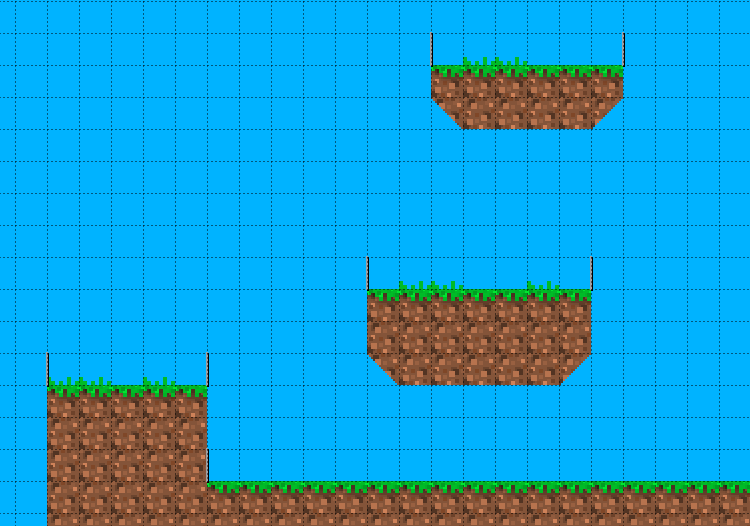
\includegraphics[width=1\textwidth]{Documentation/enemyMoveBorders}
 \caption{Invisible collision boxes that signal enemies to turn around}
 \label{fig:EnemyMoveBorders}
\end{figure}

The following method is implemented in the \texttt{EnemyMoveBorder} class. Whenever the collision listener detects, that an object of the type \texttt{Enemy} collided with a move border, this method is called and given the related enemy as a parameter.

\begin{minted}[linenos,breaklines]{java}
@Override
public void onEnemyBeginContact(Enemy enemy) {
  playScreen.log("Collision : Move border reached by enemy");
  enemy.setMovingLeftOrRight(!enemy.getIsMovingLeftOrRight());
}
\end{minted}

%------------------------------------------------

\newpage
\subsection{Using key bindings for player input} \label{DocKeyBindings}

Key bindings in games are used to give the players the possibility to individually adjust their setup as they like. Players might want to change the assigned keys for certain actions in the game, if they have unusual keyboard layouts, use other types of input devices like gamepads, or simply like to change a certain key. This gives more flexibility since hard-coded keys can cause frustration and cause an unfavourable opinion about the game.

LibGDX has two different kinds of input processing, the first one being the \texttt{Input} class included in the framework, which uses polling to get key presses. The second method is using an \texttt{InputProcessor}, also included in the framework, which uses events to control input. The key difference between those is, that one can check if a specific key is being pressed at the time of checking with the polling method. An input processor, however, triggers events when certain input events happen, like pressing down a key and then delivering the key code of the pressed key. This allows the input management to be more "clean" and efficient since one can't easily check if one of many flexible keys is being pressed without an input processor.

In order to change and save key bindings, there needs to be a data structure. This is represented in the \texttt{KeyBindingObject} class. One object each represents a single action in the game, represented by a String, and an array of integers, which represent the codes of the keys that are assigned to this action. Therefore, multiple keys can be assigned to one action.

Furthermore, the game has to save this information in a file to make it persistent, or the information will be lost once the application is closed. Therefore, the game will save and load the key bindings into a JSON (JavaScript Object Notation) file, which is a standard data interchange format. Handling this operation is done by the \texttt{KeyBindings} class. 

This class has public lists of the type Integer, which store the key codes for each individual action. These lists are read by the game to process input. In the constructor of the class, the program searches for the JSON file and if it exists, it reads it with the help of \texttt{GSON} \cite{GSON}, an open-source library by Google to convert Java Objects into JSON strings and back. If the file doesn't exist or is empty, a new one will be created and the default keys will be assigned to each action by writing them to the new file and then read them again. Those default keys are hardcoded in the constructor as a \texttt{KeyBindingObject} array.

However, if the file does exist, the JSON string is read from it and converted to an array of \texttt{KeyBindingObject}'s. Each key object will then be assigned to the proper list, that was mentioned earlier. This is done by looping through each object and adding it to the lists by comparing the String attribute, described as \texttt{}{action}. This procedure is called deserialization and can be seen in the \texttt{deserializeKeyBindings()} method of the \texttt{KeyBindings} class.

A more detailed explanation of how we utilize JSON files can be found in section \ref{DocJSONfiles}.

An exemplary key bindings JSON key binding file looks like this:

% REMOVE IF SOMETHING CHANGES
\newpage
% REMOVE IF SOMETHING CHANGES

\inputminted[linenos,breaklines]{json}{code/json/keybindings.json}

An array in JSON starts with a \texttt{[}, hence the bracket at the start and end. The \texttt{KeyBindingObject} objects in between are items of that array. Each item has a String identifier and another array for the corresponding key codes. JSON separates key and value with a \texttt{:} symbol.

As described earlier, the game uses an \texttt{InputProcessor} to handle gameplay relevant input. Since the game has to recognize when a key is pressed, and not just fire an event once a key is pressed down once, it uses public booleans to toggle between an action being active or not. Otherwise, the player would get a move impulse, for example, only once instead of for the duration of the key press. This logic is located in the \texttt{GameplayInputProcessor} class. When a key is being pressed down or being released, it checks, if the key code of the pressed key is in one of the lists. If that is the case, the \texttt{boolean} is toggled. This \texttt{boolean} is a member of the \texttt{PlayScreen} class and is \texttt{public static} to be available in this class, and is being imported in a static context, hence the missing class reference in the Input Processor class.

Finally, all of this is then used in the \texttt{update} loop of the \texttt{PlayScreen}, which is executed each frame. This is an example of the movement in the right direction:

\begin{minted}[linenos,breaklines]{java}
if (isPressingMoveRight &&
 player.body.getLinearVelocity().x <= player.getMaxWalkVelocity()) 
{
 player.body.applyLinearImpulse(new Vector2(player.getWalkImpulseVelocity(), 0), player.body.getWorldCenter(), true);
}
\end{minted}

Here, it is simply being checked, if the user presses a key that is associated with the action of moving in the right direction, by evaluating \texttt{isPressingMoveRight}. If this is the case, a linear impulse in the right direction is being applied to the player.

%------------------------------------------------

\newpage
\subsection{JSON files} \label{DocJSONfiles}

We use JSON files for many different purposes in the game, not only for storing key bindings (as described in \ref{DocKeyBindings}). The application currently manages six different JSON files: 

\begin{itemize}
  \item[\faFile] \texttt{gameprogress.json} : stores the general progress of the player in the game
  \item[\faFile] \texttt{keybindings.json} : stores the currently assigned keys to all actions in the game
  \item[\faFile] \texttt{settings.json} : stores the settings that can be changed in the menu
  \item[\faFile] \texttt{statistics.json} : stores a broad amount of statistical values
  \item[\faFile] \texttt{twitchcredentials.json} : stores the information needed to connect with the correct twitch channel
  \item[\faFile] \texttt{weaponlist.json} : stores a list of all available weapons in the game
\end{itemize}

All six cases use the same approach to reading and writing to these files. We will use the \texttt{statistics} file to explain this process. The only difference in the code is the data structure of each file.

As already mentioned in section \ref{DocKeyBindings}, the program uses the \texttt{GSON} library to serialize and deserialize all JSON files. It is very easy to use since the library can convert any Java object into the JSON format. All it needs is therefore a class that contains all variables, which the program should store.

In case of the statistics class, this is the \texttt{StatisticsObject} class. Figure \ref{fig:StatisticsObjectUML} shows the constructor and all variables inside the class.

\begin{figure}[ht]
 \center
 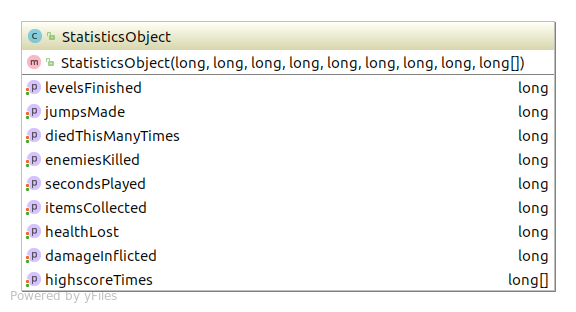
\includegraphics[width=1\textwidth]{Documentation/StatisticsObject.png}
 \caption{Statistics Object}
 \label{fig:StatisticsObjectUML}
\end{figure}

The following shortened code then shows how the structure is implemented.

\begin{minted}[linenos,breaklines]{java}
public class StatisticsObject {

  private long secondsPlayed;
  // ...
  private long[] highscoreTimes;
  
  public StatisticsObject(long secondsPlayed, /* ... */, long[] highscoreTimes) {
    this.secondsPlayed = secondsPlayed;
    // ...
    this.highscoreTimes = highscoreTimes;
  }
  
  public long getSecondsPlayed() {
    return secondsPlayed;
  }

  public void setSecondsPlayed(long secondsPlayed) {
    if (secondsPlayed >= 0) {
      this.secondsPlayed = secondsPlayed;
    }
  }
  
  // ...
}
\end{minted}

Every value is therefore passed into the constructor of the object, so every value has to be known before creating it. This is done in the only class, that uses this object and acts like the "manager" of it. In the case of the statistics, that's the \texttt{Statistics} class. This class is responsible for creating \texttt{StatisticsObject}'s and reading and writing to the JSON file.

When creating a new instance of the \texttt{Statistics} class or any other of the five managing classes, the program creates a private copy of a \texttt{StatisticsObject} by reading the data from the JSON file or writing default values to it, if it doesn't exist or is empty, and then reading from it again. The class then implements getters and setters for each property of the data structure. The getters simply return the values of the properties by calling the lower-level getter of the private \texttt{StatisticsObject} instance. The setter changes the new value in the private instance of the \texttt{StatisticsObject} and then write the changes to the file. With this strategy, the user only has to create one instance of the managing class and can then easily get and set values without having to worry about writing and reading from the file.

The following declaration of three variables in the \texttt{Statistics} class is the beginning of said class. The \texttt{File Handle} is a libGDX class that handles file operations, the \texttt{GSON} class is responsible for serializing and deserializing the objects into JSON strings, and the \texttt{StatisticsObject} is the previously described private copy of the data in the file.

\begin{minted}[linenos,breaklines]{java}
private FileHandle fileHandle;
private Gson gson = new GsonBuilder().setPrettyPrinting().create();
private StatisticsObject statistics;
\end{minted}

The following constructor then takes care of the initial reading of the file. A \texttt{StatisticsObject} with default values is created here, in case the wanted file doesn't exist or is empty. The logic then examines if the file exists or not. And if it does, and is also not empty, the method \texttt{deserializeStatistics()} is called, which reads the data from the file and stores it in the private copy of a \texttt{StatisticsObject}. In any other case, the method \texttt{serializeStatistics()} is called with the parameter of the default values, which writes the given values to the file and creates a new file, if it doesn't exist.

\begin{minted}[linenos,breaklines]{java}
public Statistics() {
  fileHandle = Gdx.files.local("json/statistics.json");
  StatisticsObject defaultStatistics = new StatisticsObject(
      0, 0, 0, 0, 0, 0, 0, 0, new long[MainGameClass.NUMBER_OF_LEVELS]
  );

  if (fileHandle.exists()) {
    String json = fileHandle.readString();
    if (!json.trim().isEmpty()) {
      statistics = deserializeStatistics(json);
    } else {
      System.err.println("JSON statistics string is empty, creating default statistics");
      serializeStatistics(defaultStatistics);
      statistics = deserializeStatistics(json);
    }
  } else {
    serializeStatistics(defaultStatistics);
    statistics = deserializeStatistics(fileHandle.readString());
  }
}
\end{minted}

The below method \texttt{serializeStatistics()} finally converts the data structure into a JSON string using the \texttt{GSON} library. Before writing that string to the file, the method examines if the file exists, and if it doesn't, it will create a new file. This is done in a try-catch block in order to avoid crashes if the file creation fails. This should always be done when handling files, as they are prone to errors. After that, the string will finally be written to the file and the private copy of the \texttt{StatisitcsObject} will be updated by reading the just written data back from the file, using the \texttt{deserializeStatistics()} method.

\begin{minted}[linenos,breaklines]{java}
private void serializeStatistics(StatisticsObject statistics) {
  String json = gson.toJson(statistics);

  if (!fileHandle.exists()) {
    try {
      boolean successfull = fileHandle.file().createNewFile();
    } catch (IOException e) {
      e.printStackTrace();
    }
  }

  fileHandle.writeString(json, false); // false = overwrite instead of append
  this.statistics = deserializeStatistics(json);
}
\end{minted}

The below method \texttt{deserializeStatistics()} simply returns an \texttt{StatisticsObject} instance by converting a JSON formatted string into the data structure with the help of \texttt{GSON}. The second paramter tells \texttt{GSON}, which type of data it is supposed to convert to.

\begin{minted}[linenos,breaklines]{java}
private StatisticsObject deserializeStatistics(String json) {
  return gson.fromJson(json, StatisticsObject.class);
}
\end{minted}

As the last thing in this class, we can now finally get and set values in our data structure by calling the appropriate getters and setters. The below example shows one each since they all follow the same logic. The getter simply returns the value by calling the getter of the data structure. The setter changes correct value in the private instance of the \texttt{StatisticsObject} class and then writes the changes to the file.

\begin{minted}[linenos,breaklines]{java}
public long getSecondsPlayed() {
  return statistics.getSecondsPlayed();
}

public void setSecondsPlayed(long secondsPlayed) {
  statistics.setSecondsPlayed(secondsPlayed);
  serializeStatistics(statistics);
}
\end{minted}

 %------------------------------------------------

\newpage
\subsection{Animations} \label{DocAnimations}

An animation can be described as the illusion of movement caused by rapidly switching between different static images. We animated our characters by using libGdx's \texttt{Animation} Class \cite{libGdxAnimClass}. An animation consists of multiple frames which are shown in a sequence at set intervals. The Animation Class stores a list of objects representing the sequence. Each object in the Animation is called a keyframe, and multiple keyframes make up the animation.

A typical 2D animation consists of a number of TextureRegions and would be specified as:

\mint{java}{Animation<TextureRegion> myAnimation = new Animation<TextureRegion>(...);}

Every animation needs a sprite sheet - that's an image consisting of all the frames for the animation. A sprite sheet can contain more than one animation, so each animation is described in a texture atlas file, refer to the Sprites section in the Technical documentation for more information. 

All the texture atlases are defined in the game's \texttt{PlayScreen} class, using the following syntax:

\begin{minted}[linenos,breaklines]{java}
//Define frog atlas
enemyFrogTextureAtlas = new TextureAtlas("sprites/enemies/frog/frog.atlas");
\end{minted}

\begin{minted}[linenos,breaklines]{java}
//Frog atlas getter
public TextureAtlas getEnemyFrogTextureAtlas() {
 return enemyFrogTextureAtlas;
}
\end{minted}

The defined atlases can be reached from other classes via a getter.

We created the actual animations in the class for each specific character. 

The first step is to add all the frames we'll need into an array, by selecting the start of the animation from the texture atlas and iterating until we have collected all the frames (in this case the frames are 4).

The second step is to pass the speed of the animation to the Animation Class along with the animation frames.

\begin{minted}[linenos,breaklines]{java}
//Define jump animation
jumpFrames = new Array<>();
for(int i = 0; i < 4; i++) {
 jumpFrames.add(new TextureRegion(
  screen.getEnemyFrogTextureAtlas().findRegion("frog_jump"), i * ENEMY_PIXEL_WIDTH, 0, ENEMY_PIXEL_WIDTH, ENEMY_PIXEL_HEIGHT)
 );
}
jumpAnimation = new Animation<>(0.4f, jumpFrames);
\end{minted}

It's up to the developer though to specify when and for how long the animation is run. In our case, we jump animation is in a continuous loop, and the attack is used only when the enemy and player are in contact.

\begin{minted}[linenos,breaklines]{java}
public void update(float deltaTime) {
 setRegion(jumpAnimation.getKeyFrame(stateTime, true));
}
\end{minted}

%------------------------------------------------

\newpage
\subsection{Weapon collecting} \label{DocWeaponCollection}

When they player comes in contact with a weapon the item is added to the player's weapon collection. The logic behind that feature has been implemented in the \texttt{WeaponPickup} class. Every time the player collides with an enemy, the \texttt{onPlayerBeginContact} method is called, which detects what kind of weapon the player has picked up and adds it to the weapon's list if it is not already present. The weapon type is setup in the map. When setting up the map, each object of the map's object layers can be given custom properties. In the case of the weapons - we added properties containing the type of the weapon. This makes it easier to identify the contents programatically.

\begin{figure}[ht]
 \center
 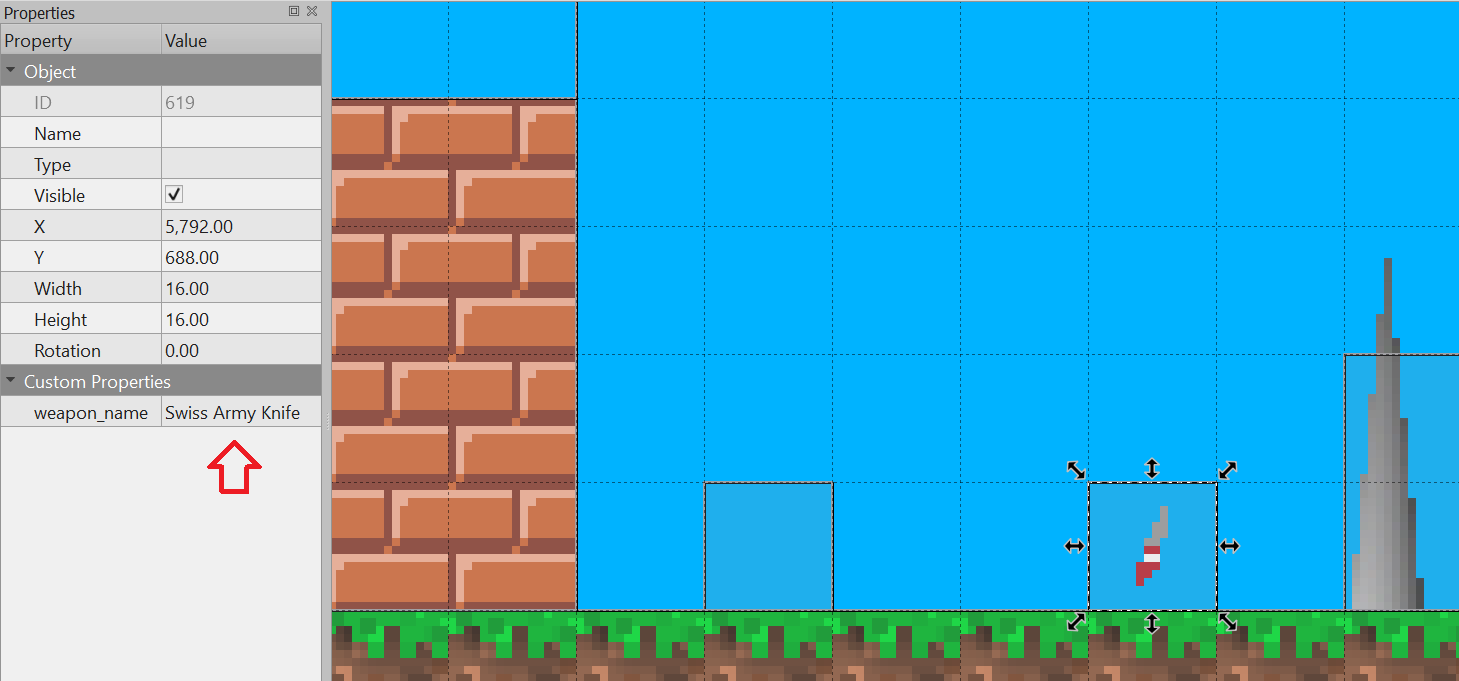
\includegraphics[width=1\textwidth]{Documentation/weaponMaps.png}
 \caption{Custom property of a weapon in a map}
\end{figure}

After the item is picked up, the \texttt{onPlayerBeginContact()} method detects it's type and the texture is removed from the map and added to the player's weapon list if it has not been added already.

\begin{minted}[linenos,breaklines]{java}
 public void onPlayerBeginContact(Player player) {
  // Remove texture
  getCell(map.getLayers().getIndex("graphics")).setTile(null);

  // Add the picked up weapon
  MapObject pickedUpWeapon = getCollidingMapObject(map.getLayers().getIndex("weapon"));
  
  if (pickedUpWeapon != null && pickedUpWeapon.getProperties().containsKey("weapon_name")) {
  
   String weaponName = pickedUpWeapon.getProperties().get("weapon_name", String.class);
   playScreen.log("Picked up weapon: " + weaponName);

   boolean changedWeaponList = false;
   ArrayList<WeaponObject> playerWeaponList = playScreen.getPlayer().getWeapons();
   WeaponObject weapon;
   
   switch (weaponName) {
    case "Fists":
     weapon = getWeaponObjectByName("Fists");
     if (weapon != null && !weaponAlreadyInList(weapon)) {
      playerWeaponList.add(weapon);
      changedWeaponList = true;
     }
     break;
    // Several cases were omitted here to save space
    default:
     playScreen.log("Weapon not defined");
     break;
   }

   if (changedWeaponList) {
    playScreen.getPlayer().setWeapons(playerWeaponList);
    playScreen.getPlayer().changeWeapon(weaponName);

    // Save picked up item to statistics
    playScreen.getStatistics() .setItemsCollected(playScreen.getStatistics().getItemsCollected() + 1);
   }
  }
 }
\end{minted}
 
The \texttt{getCollidingMapObject} method can be found in the \texttt{InteractiveMapTileObject} class. It's purpose is to return the object in a specific layer, that is currently intersecting with the player's collision box. The returned object stores all properties, including the custom property that contains the weapon name of the object. It is unfortunately not possible to check for collisions with weapon pick up items using the \texttt{Contact Listener}, because it is impossible to identify the exact object of the map that the player collided with. This can be therefore considered a workaround.
 
\begin{minted}[linenos,breaklines]{java}
protected MapObject getCollidingMapObject(int layerIndex) {
  MapObjects mapObjects = map.getLayers().get(layerIndex).getObjects();

  for (MapObject mapObject : mapObjects) {
    MapProperties mapProperties = mapObject.getProperties();

    float width, height, x, y;
    Rectangle objectRectangle = new Rectangle();
    Rectangle playerRectangle = new Rectangle();

    if (mapProperties.containsKey("width") && mapProperties.containsKey("height") && mapProperties.containsKey("x") && mapProperties.containsKey("y")) {
      width = (float) mapProperties.get("width");
      height = (float) mapProperties.get("height");
      x = (float) mapProperties.get("x");
      y = (float) mapProperties.get("y");
      objectRectangle.set(x, y, width, height);
    }

    playerRectangle.set(
        playScreen.getPlayer().getX() * MainGameClass.PPM,
        playScreen.getPlayer().getY() * MainGameClass.PPM,
        playScreen.getPlayer().getWidth() * MainGameClass.PPM,
        playScreen.getPlayer().getHeight() * MainGameClass.PPM
    );

    // If the player rectangle and the object rectangle is colliding, return the object
    if (Intersector.overlaps(objectRectangle, playerRectangle)) {
      return mapObject;
    }
  }

  // If no colliding object was found in that layer
  return null;
}
  
\end{minted}

%------------------------------------------------

\newpage
\subsection{Sprites} \label{DocSprites}

Historically, the retro 8-bit games have always been very minimalist, in terms of the animations of the characters. Luckily the designs we used for our textures, described in the Visual Documentation, already had suitable animations. We just needed to convert the animated GIFs to sprite sheets. A sprite sheet is a series of images of the frames that represent the animation. A gif can be converted to a sprite sheet with the use of an online sprite editor, Piskelapp \cite{piskelapp}. Although the process is automated, the resulting spritesheet had excess frames, which need to be removed. This is the end result.

\begin{figure}[ht]
 \center
 
\includegraphics[width=1\textwidth]{Documentation/frog.jpg}
 \label{SpriteSheetExample}
 \caption{Sprite Sheet Example}
\end{figure}

Sprite sheets can contain more than one animation, and even multiple characters. For instance, in the case of the frog enemy, the sprite sheet contains two different animations - the first 4 frames from left to right are used to animate movement. The last 4 are used for the attack animation. To help select the correct parts of the sprite sheet while animating, a \texttt{TextureAtlas} is generated. Among other information about the sheet, it contains the start position of the two types of animation. Here is an example:

\begin{minted}[linenos,breaklines]{text}
frog.png
size: 256, 32
format: RGBA8888
filter: Nearest,Nearest
repeat: none
frog_jump
 rotate: false
 xy: 0, 0
 size: 128, 32
 orig: 128, 32
 offset: 0, 0
 index: -1
frog_attack
 rotate: false
 xy: 128, 0
 size: 128, 32
 orig: 128, 32
 offset: 0, 0
 index: -1
\end{minted}

The described process above was repeated for all the characters in our game. 

For an explanation on how the atlas is used and the game engine renders the animations - refer to the Animations section in the Technical Documentation.

%------------------------------------------------

\newpage
\subsection{Maps} \label{DocMaps}

After making a map in the \texttt{Tiled} map editor, we exported it to a .tmx file and used it in the project. A TMX file contains all the map’s custom properties and all the layers, which have been made in the map editor. The following code is an example of how the .tmx file is loaded when starting a new level.

\begin{minted}[linenos,breaklines]{java}
mapLoader = new TmxMapLoader();

switch (gameProgress.getCurrentLevel()) {
 case 1:
  map = mapLoader.load("maps/level_1/level_1.tmx");
  break;
 case 2:
  map = mapLoader.load("maps/level_2/level_2.tmx");
  break;
 case 3:
  map = mapLoader.load("maps/boss/boss_level.tmx");
  break;
 default:
  game.exitApplication("Couldn't find level, exiting application");
  break;
}
\end{minted}

The above code creates an instance of the map and loads the current level by reading the JSON file (see section \ref{DocJSONfiles}). If the current level is set to one, it loads the first level. If the current level is set to two then loads the second level, and so on.

The following constructor of the class \texttt{Box2DWorldCreator} reads out the object layers of the map and creates the relevant objects in the physics simulation. Only rectangular objects are considered.

% REMOVE IF SOMETHING CHANGES
\newpage
% REMOVE IF SOMETHING CHANGES

\begin{minted}[linenos,breaklines]{java}
public Box2DWorldCreator(PlayScreen screen) {
    this.playScreen = screen;
    TiledMap map = screen.getMap();
    MapLayers mapLayers = map.getLayers();
    for (MapLayer mapLayer : mapLayers) {
      for (MapObject mapObject : mapLayer.getObjects().getByType(RectangleMapObject.class)) {
        Rectangle rectangle = ((RectangleMapObject) mapObject).getRectangle();
        switch (mapLayer.getName()) {
          case "ground":
            groundObjects.add(new Ground(screen, rectangle));
            break;
          // Other types omitted because of redundancy
          default:
            break;
        }
      }
    }
  }
\end{minted}

%------------------------------------------------

\newpage
\subsection{Head-up display} \label{DocHUD}

The head-up display consist of several elements, which are:

\begin{itemize}
  \item A timer that shows the current game time and is counting up
  \item A health bar
  \item A label to display the player's remaining lives
  \item A label to display the strength of the currently equipped weapon
  \item A label to display the remaining time of an active effect by Twitch (see section \ref{Twitch})
\end{itemize}

As described in the discussion (see section \ref{Discussion}), we also wanted to add a toolbar to show all the weapons that the player has in his inventory, and in which slots they are. This failed due to the time limitation.

LibGDX uses \texttt{Scene2D} \cite{Scene2DUI} to realize low levels of UI's. It has several widgets available and uses a table system to layout the elements. However, the visual side of these widgets have to be defined manually with something called \texttt{Skins}. A skin can contain the required fonts and define, which font, color and graphic to use for which widget and for which state of it. This is not as easy as it sounds, because it is not very well documented and there are no templates available. Luckily, we found a tool called "Skin Composer" \cite{SkinComposer} which simplifies the creation of the necessary files.

The output of this tool are several PNG files which contain all graphics, packed together in the most efficient way. A texture atlas then describes the different texture regions by coordinates. Texture atlases were also used for the player textures and enemy textures (see section \ref{DocAnimations}). The actual skin file is a JSON file with special syntax, which describe each state of each widget. The following snippet is from that JSON file and describes the appearance for \texttt{ImageTextButtons}, which are used for the display of the remaining lives and weapon strength.

\begin{minted}[linenos,breaklines]{text}
com.badlogic.gdx.scenes.scene2d.ui.ImageTextButton\$ImageTextButtonStyle: {
	default: {
		font: PressStart2P
		fontColor: white
	}
	lifes: {
		imageUp: heart_icon
		font: PressStart2P
		fontColor: white
	}
	weapon_strength: {
		imageUp: weapon_strength_icon
		font: PressStart2P
		fontColor: white
	}
}
\end{minted}

The documentation on the creation of HUD graphics can be found in the visual documentation in section \ref{VisualDocumentation}.

The \texttt{PlayScreenHud} class implements all this by creating a new viewport and adding a so called \texttt{Stage}, which can have multiple \texttt{Actors}. The only actor it will have, is the layout table that contains all elements of the HUD.

The table is initialized by the following code:

\begin{minted}[linenos,breaklines]{java}
Table layoutTable = new Table();
layoutTable.top();
layoutTable.setFillParent(true);
layoutTable.pad(getPixelSizeFromDensityIndependentPixels(50));
\end{minted}

The \texttt{top()} method defines, that the order is from top to bottom. \texttt{setFillParent(true)} sets the size of the table to the entire screen and \texttt{pad()} adds a padding to each side of the screen so that all elements have a certain distance to the edge of the screen.

The skin is initialized by reading it from the JSON file:

\begin{minted}[linenos,breaklines]{java}
skin = new Skin(Gdx.files.internal("skins/hud/hud.json"));
\end{minted}

The widgets have to be initialized with the styles now. The progress bar is created by the following code:

\begin{minted}[linenos,breaklines]{java}
healthBar = new ProgressBar(
  0f,
  playScreen.getGameProgress().getPlayerMaxHealth(),
  1f,
  false,
  skin,
  "default-horizontal"
);
\end{minted}

The parameters are the minimum value, the maximum value, the step size, if it is vertical, the skin and the style name in the skin.

The following code then defines the layout of the table and assigns the widgets to it.

\begin{minted}[linenos,breaklines]{java}
layoutTable.add(healthBar).expandX().growX().left().top().spaceBottom(25);
layoutTable.add(new Actor()).expandX().fillX().center().top().spaceBottom(25);
layoutTable.add(timerLabel).expandX().right().top().spaceBottom(25);
layoutTable.row();
layoutTable.add(lifesImageTextButton).expandX().left().top().spaceBottom(10);
layoutTable.row();
layoutTable.add(weaponStrengthImageTextButton).expandX().left().top().spaceBottom(10);
\end{minted}

The stacked up methods after the addition of a widget define the behaviour of the item in the table.

The set-up is now complete and the table can be added to the \texttt{Stage}, which will then be drawn over the play screen.

\begin{minted}[linenos,breaklines]{java}
stage.addActor(layoutTable);
\end{minted}

When updating the HUD each frame, the widgets can be directly modified and it will be automatically show up. For example, when updating the progress bar, this line of code is used:

\begin{minted}[breaklines,linenos]{java}
healthBar.setValue(playScreen.getPlayer().getHealth());
\end{minted}

%------------------------------------------------

\newpage
\subsection{Menus} \label{DocMenus}

The main menu system consists of four different screens:

\begin{itemize}
  \item the main menu
  \item the level selection menu
  \item the settings menu
  \item the statistics menu
\end{itemize}

Each screen is \texttt{extends} the \texttt{abstract} \texttt{MenuScreen} class. This class loads the \texttt{Skin} of the template that we use (see section \ref{VisualDocMenus}), creates an empty layout table and handles rendering and other methods that a \texttt{Screen} needs to override.

Each child class can now simply extend this class and create widgets to add to the layout table. As an example, we can take a look at the \texttt{MainMenu} class, which displays four different buttons: \emph{Play}, \emph{Settings}, \emph{Statistics} and \emph{Exit}. A screenshot of the menu can be found in the visual documentation of the menus (see section \ref{VisualDocMenus}).

A \texttt{TextButton} can be created with the following constructor, giving three parameters: The text on the button, the \texttt{Skin} and the name of the style in the skin, which is "\texttt{default}" in this case. Each widget can have several styles in a \texttt{Skin}.

\mint{java}{playButton = new TextButton("Play", skin, "default");}

To add a button or any other widget to the menu, it has to be added to the layout table that will be added as an \texttt{Actor} to the \texttt{Stage}. This was briefly described in the documentation of the head-up display (see section \ref{DocHUD}). The following code snippet adds the play button to the table with two empty actors to the left and right that share the space, so the button doesn't take up the entire width of the screen.

\begin{minted}[linenos,breaklines]{java}
layoutTable.add(new Actor())
  .expandX()
  .spaceBottom(getPixelSizeFromDensityIndependentPixels(25f));
layoutTable.add(playButton)
  .top().center().growX().expandX()
  .spaceBottom(getPixelSizeFromDensityIndependentPixels(25f));
layoutTable.add(new Actor())
  .expandX()
  .spaceBottom(getPixelSizeFromDensityIndependentPixels(25f));
layoutTable.row();
\end{minted}

The last thing to do now is to add event listeners to the widgets. For example, the checkbox will have a \texttt{change} listener, the buttons will have \texttt{click} listeners, and so on.

\begin{minted}[linenos,breaklines]{java}
private ChangeListener fullscreenCheckBoxChangeListener = new ChangeListener() 
{
  @Override
  public void changed(ChangeEvent event, Actor actor) {
    settings.setFullscreen(fullscreenCheckBox.isChecked());
    game.changeGameResolution();
  }
};
\end{minted}

This change listener first toggles the value in the settings file, depending on if the checkbox is checked or not. After that, the method \texttt{changeGameResolution} is called which reads the settings from the JSON file and then changes the application's resolution based on it.

Since the change listener is simply an object of the type \texttt{ChangeListener}, it can be added to a widget like this:

\mint{java}{fullscreenCheckBox.addListener(fullscreenCheckBoxChangeListener);}

Navigating through the menus is generally done by simply creating new instances of the relevant screen and assigning it to the instance of the main game class as the next screen.

The following flowchart shows the navigation within the menus of the game.

\begin{figure}[ht]
 \center
 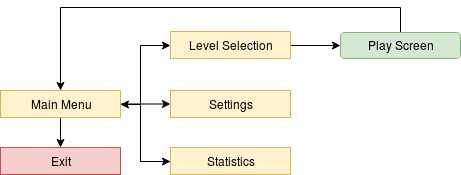
\includegraphics[width=1\textwidth]{Documentation/flowchart.png}
 \label{fig:flowchart}
 \caption{Flowchart of the menus}
\end{figure}

%------------------------------------------------

\subsection{Highscore system} \label{Highscore}

For the highscore system we made a PHP/SQL API to be accesed at the end of a level. The API takes 3 inputs: level, time, name. Whenever a level ends, a HTTP post call is sent to the API with the current level, the time it took to complete the level, and the username from the \texttt{settings.json} file. Sending the data this way is not very secure, and since anyone could easily fake a high score it is not very reliable either. In order to improve security we would like to obfuscate the sent data, or implement an account system of sorts, requiring you to login to submit your highscore.

\begin{figure}[ht]
 \center
 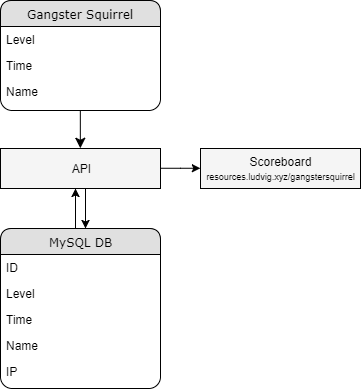
\includegraphics[width=0.5\textwidth]{Documentation/gsapi.png}
 \label{fig:highscoresystem}
 \caption{Flowchart of the API}
\end{figure}

\begin{minted}[linenos,breaklines]{java}
// http post code from: https://stackoverflow.com/a/16284863/5645395

HttpClient httpClient = new DefaultHttpClient();
HttpPost httpPost = new HttpPost("http://api.ludvig.xyz/gangstersquirrel/");

List<NameValuePair> params = new ArrayList<NameValuePair>();
params.add(new BasicNameValuePair("level", String.valueOf(gameProgress.getCurrentLevel())));
params.add(new BasicNameValuePair("name", gameProgress.getPlayerName()));
params.add(new BasicNameValuePair("time", String.valueOf(timer)));

httpPost.setEntity(new UrlEncodedFormEntity(params, "UTF-8"));
HttpResponse response = httpClient.execute(httpPost);
HttpEntity respEntity = response.getEntity();

if (respEntity != null) {
  // EntityUtils to get the response content
  String content = EntityUtils.toString(respEntity);
}
\end{minted}

%------------------------------------------------

\newpage
\subsection{Twitch} \label{Twitch}

Twitch.tv is a live streaming platform with 15 million daily active users \cite{twitchAbout}, it features an IRC chat alongside the live stream so the viewers can interact with the livestreamer. Twitch has a few emotes defined in the IRC chat, for example, if you type "Kreygasm" in the chat, a little face appears.

\begin{figure}[ht]
 \center
 
\includegraphics[width=0.05\textwidth]{Documentation/Kreygasm.png}
 \label{Kreygasm_emote}
 \caption{Kreygasm emote on Twitch \cite{TwitchEmotes}}
\end{figure}

A few newer games, such as Jackbox games \cite{JackboxGames} have added twitch integration to their games, meaning what the viewers say in chat affects the game the streamer is playing. Using a Java IRC framework called Pircbot \cite{pircbot} we can connect to the twitch IRC server. In order to not have the IRC connection slow down the rest of the game, we start a separate thread for handling the IRC connection. We use an \texttt{interface} to listen to the chat and call a function in the \texttt{TwitchChat} object whenever a messaged is received.

\begin{minted}[linenos,breaklines]{java}
public interface ChatListener {
  void messageReceived(String channel, String sender,
             String login, String hostname, String message);
}
\end{minted}

In the TwitchThread class, we can define what should happen upon receiving a message. We have a predefined list of messages, which will perform an action in the game, for now, the only action implemented is lowering gravity on the emote "Kreygasm", but the system is built in a way where we could easily implement more actions.

\begin{minted}[linenos,breaklines]{java}
private ArrayList<String> receivableMessages = new ArrayList<>();
public TwitchThread(boolean enabled, MainGameClass mainGameClass)
{
  // ...
  receivableMessages.add("Kreygasm");
}
\end{minted}

In the \texttt{TwitchThread} class we implement our \texttt{ChatListener} object and define the method for receiving a message. When we receive a message we add it to a log of the last 10 messages. When the program receives a message, it checks the log of the 10 messages, if 3 of the last 10 messages were in the \texttt{receivableMessages} list we call a method in the \texttt{MainGameClass}.

\begin{minted}[linenos,breaklines]{java}
public void messageReceived(String channel, String sender, String login, String hostname, String message) {
  for (String receivableMessage : receivableMessages) {
    if (getNumberOfThisMessagesInLog(twitch.getLog(), receivableMessage) >= 3) {
      mainGameClass.receiveActionFromTwitch(receivableMessage);
    }
  }
}
\end{minted}

The action for a message in \texttt{receivableMessages} is defined in the \texttt{MainGameClass}. We first check if the current screen is the \texttt{PlayScreen}, after that, we check for which action to perform and then add the effect by defining the \texttt{effectStateTime}, and \texttt{currentEffect}, then we apply the actual effect, which for the "Kreygasm" emote is changing the gravity.

\begin{minted}[linenos,breaklines]{java}
public void receiveActionFromTwitch(String action) {
	if (this.getCurrentScreen().isPresent() && this.getCurrentScreen().get() instanceof PlayScreen) {
		playScreen = (PlayScreen) this.getCurrentScreen().get();

		if (action.equalsIgnoreCase("Kreygasm")) {
		  if (playScreen != null) {
		    effectStateTime = 0f;
		    currentEffect = "Kreygasm";
        playScreen.getWorld().setGravity(new Vector2(0, - GRAVITY / 2));
      }
		}
	}
}
\end{minted}

The \texttt{getCurrentScreen} method returns a \texttt{Screen} instance encapsulated in the new \texttt{Optional} object, which was introduced in Java SE 8 \cite{JavaOptional}. We could obviously just use the \texttt{getScreen} method of libGDX and check, if the returned object is not null, but we wanted to test out the newest try of Oracle to unf**k null pointers in Java. The following snippet is the getter to receive the \texttt{Optional}.

\begin{minted}[linenos,breaklines]{java}
public Optional<? extends Screen> getCurrentScreen() {
  return Optional.of(this.getScreen());
}
\end{minted}

After a set amount of time we will remove the effect again.

\begin{minted}[linenos,breaklines]{java}
private float maximumEffectTimeInSeconds = 15f
public void updateTwitchEffectTimer() {
  if (effectStateTime >= maximumEffectTimeInSeconds) {
    effectStateTime = 0f;

    switch (currentEffect) {
      case "Kreygasm":
        playScreen.getWorld().setGravity(new Vector2(0, - GRAVITY));
        break;
      default:
        break;
    }
  }
}
\end{minted}

%----------------------------------------------------------------------------------------
%	PLAYTESTING AND SURVEY RESULTS
%----------------------------------------------------------------------------------------

\newpage
\section{Playtesting and Survey results}

In this section we would like to briefly describe our playtesting process and the survey results that we got afterwards.

Playtesting:
"A playtest is the process by which a game designer tests a new game for bugs and design flaws before bringing it to market." \cite{Playtest}



%----------------------------------------------------------------------------------------
%	DISCUSSION
%----------------------------------------------------------------------------------------

\newpage
\section{Discussion} \label{Discussion}

Although we did a lot of planning and divided task equally among the team we didn't have enough time to accomplish a lot of features we wanted our game to have. That's more due to the limited time we had at our disposal that anything else, but if we had an opportunity to continue the project we would do the following:

\begin{itemize}
  \item Design our own sprites - we used animated images we found online to build the enemies in our game. This saved us a lot of time and effort, but ideally we would like to build them ourselves so they are more fitting to the overall theme of the game.
  \item Add more levels - we were only able to make 3 maps, which makes our game quite short. Ideally we would like to add more levels when our player is climbing the tree to get to the top.
  \item Experience points - ideally we would have wanted our hero to be able to have different characteristics (strength, agility, stamina, etc) that can be improved as the game progresses and our player gains experience and levels up.
  \item Weapon toolbar - integrating our weapons list as a tool belt where players can see what weapons they have available, the shortcuts that allow them to equip each weapon 
  \item More weapons - we planned to add ranged weapons as well, which would make the game more interesting and incentivize users to play longer.
  \item More items - initially we wanted to allow our player access to equipment that will help him during the game. Items that will increase his speed, jump distance or other special abilities.
  \item Prizes - we wanted to allow our player to pick up coins and different prizes that add up to your score.
  \item Climbing - currently our player can only move left and right, and also jump. We would like to add the ability to him to climb ladders, ropes, etc.
\end{itemize}

%----------------------------------------------------------------------------------------
%	CONCLUSION
%----------------------------------------------------------------------------------------

\newpage
\section{Conclusion}

In the introduction of this report, we formulated a goal for this project. In this section we will conclude whether we achieved the goal or not. The project's goal was as following:

\textit{How can we develop a retro game using one of the modern game engines? What platforms should it support and what price should it have?}

During our research, we were surprised to see how much the game industry has grown since it's beginning, both in variety and popularity. A decade ago games were more of a niche hobby, but the latest industry reports show that it has become a new entertainment sector of considerable size.

This growth has brought a lot of success to a lot of game developers, and it's become harder to develop a competitive game, due to the contenders. The market has become very competitive and increasingly saturated.

Users expect high quality products, which is one of the reasons we developed our game with a modern game engine (libGDX), which helped us save time and make the game run smoothly. The library allowed us to design the game ourselves, which enabled us to achieve the retro look we aimed for.

Another advantage of using libGDX was that it can run on multiple platforms. Each platform hold an almost equal market share and the use of a game engine can help us reach more of the consumers. That's why we decided to release our game for these platforms, chosen on the basis of compatibility:

\begin{itemize}
  \item Microsoft Windows
  \item macOS
  \item Linux
\end{itemize}

Last but not least, we've set a price for our product as following: 

\begin{itemize}
 \item All platforms: 3.99\$ USD
\end{itemize}

Though you can build a game without any external libraries, our experience led us to believe that you'd be doing yourself a disservice, if you don't use tools that help you save resources and provide a higher quality product.

%----------------------------------------------------------------------------------------
%	BIBLIOGRAPHY
%----------------------------------------------------------------------------------------

\newpage
\printbibliography[heading=bibintoc,title={References}]

%----------------------------------------------------------------------------------------
%	APPENDIX
%----------------------------------------------------------------------------------------

\newpage
\appendix

\section{Appendix}

\subsection{Class diagram} \label{AppendixClassDiagramFull}

The following figure is the full class diagram of the entire project. A high resolution version can be found here: \texttt{https://i.imgur.com/goEseUO.png}

\begin{figure}[ht]
 \centering
 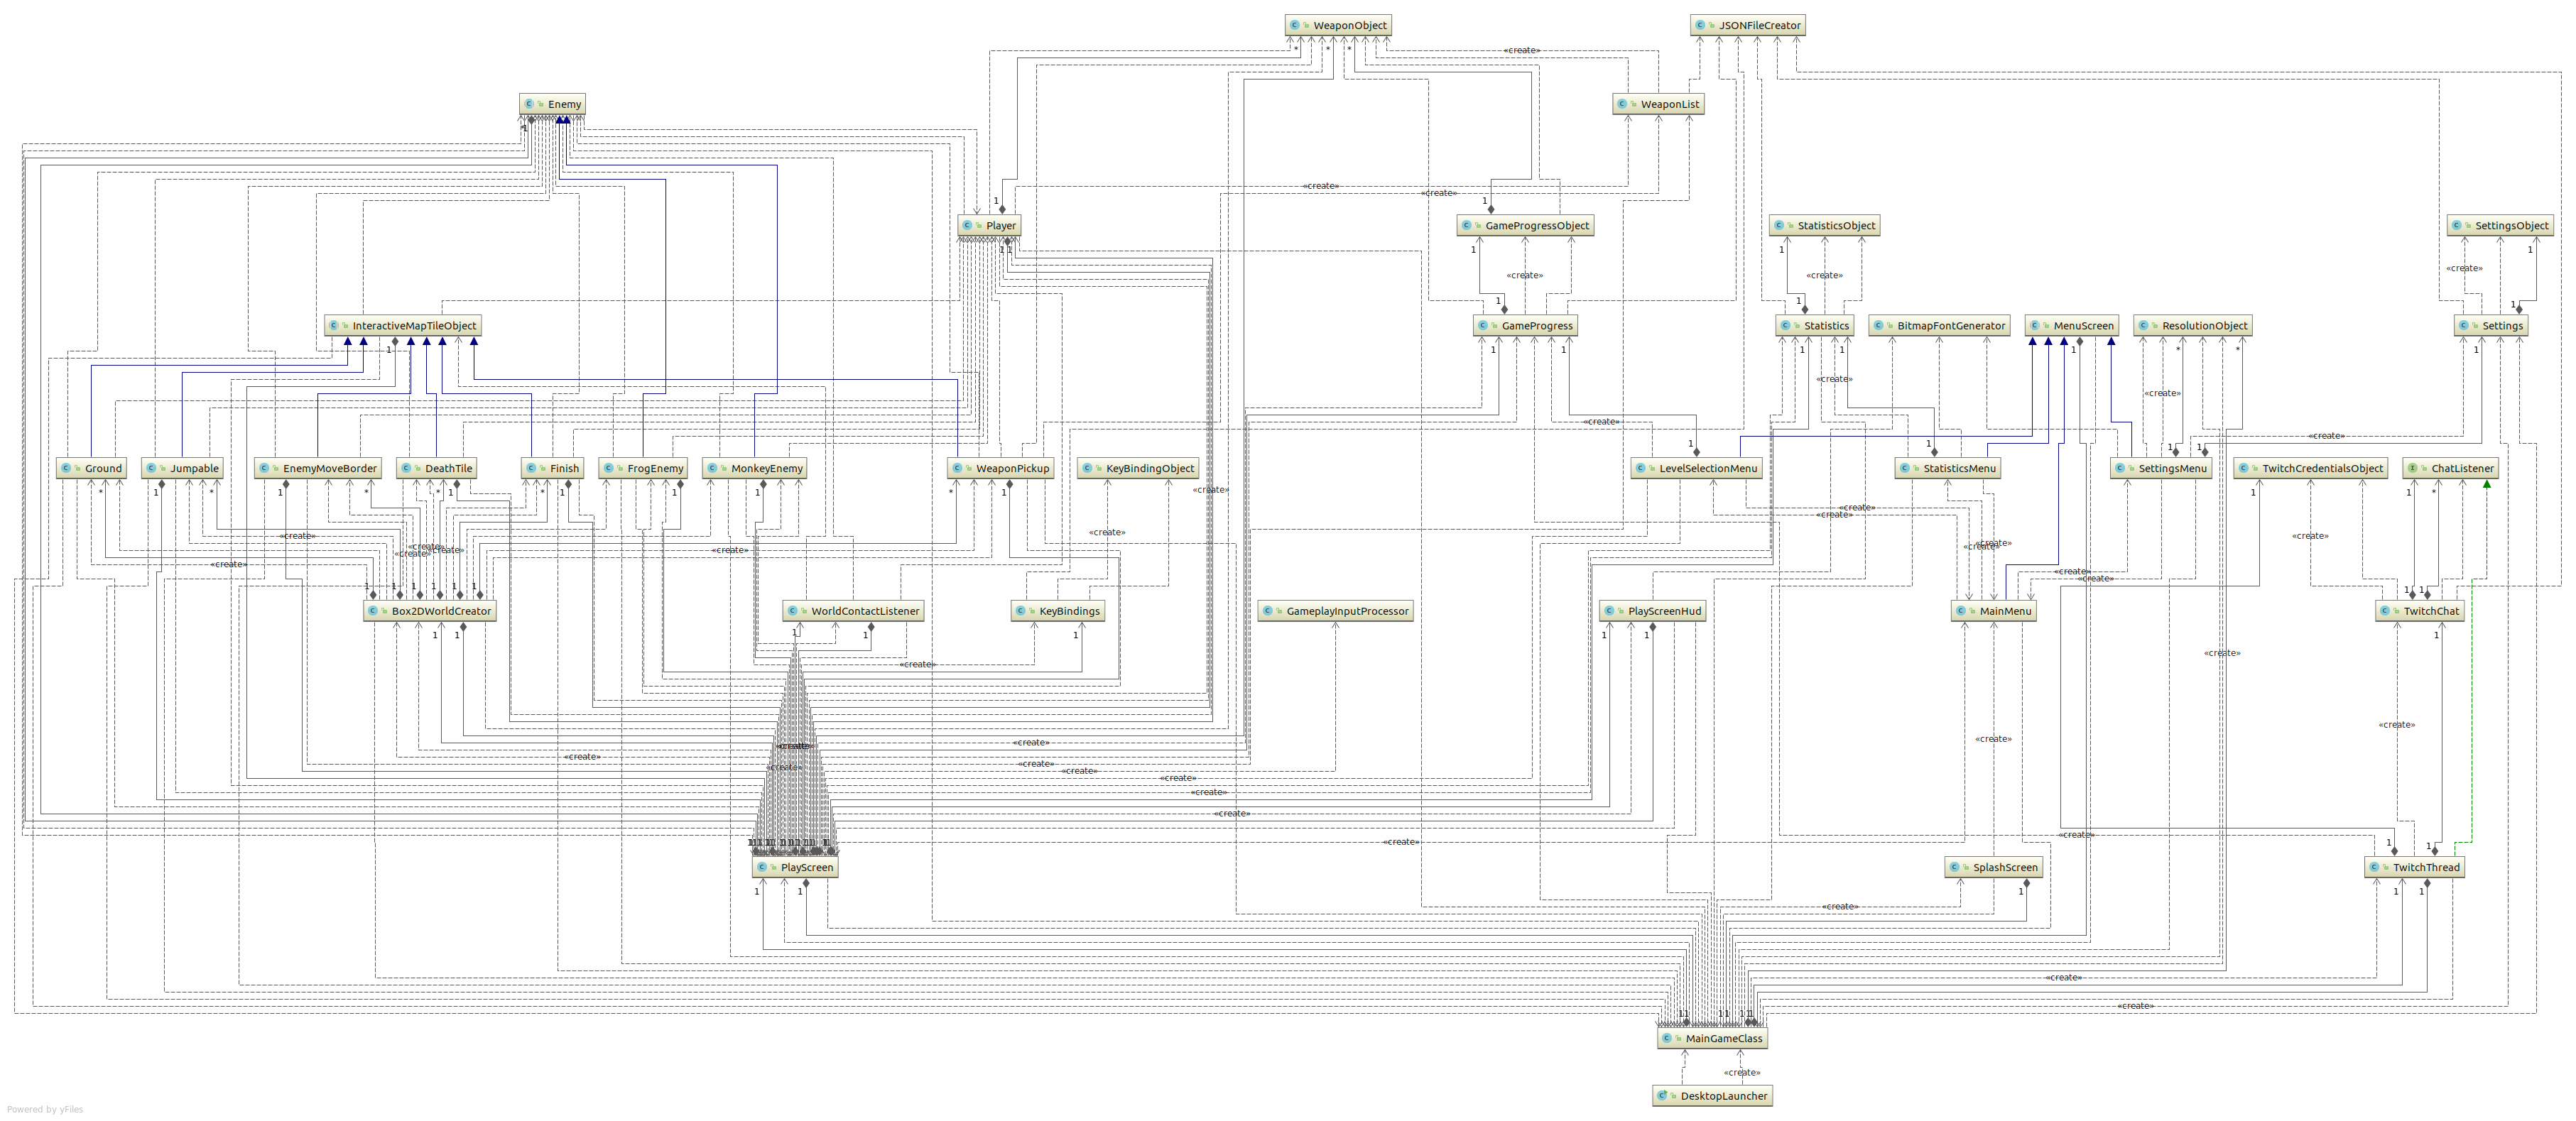
\includegraphics[width=1\textwidth]{Documentation/class_diagram}
 \caption{Full class diagram}
 \label{fig:ClassDiagramFull}
\end{figure}

%------------------------------------------------

% REMOVE IF SOMETHING ABOVE CHANGES
\newpage
% REMOVE IF SOMETHING ABOVE CHANGES
\subsection{Source Code} \label{SourceCode}

The following appendix contains direct links to each Java class file and possibly other relevant files on the GitHub repository since the raw code is too long to put here.

\renewcommand{\labelitemi}{\faFolderOpen}
\renewcommand{\labelitemii}{\faFile}
\renewcommand{\labelitemiii}{\faFile}
\begin{itemize}
  \item \textbf{/}
  \begin{itemize}
    \item MainGameClass: \url{https://goo.gl/sWmPjR}
  \end{itemize}
  
  \item \textbf{GameProgress}
  \begin{itemize}
    \item GameProgress: \url{https://goo.gl/2RTmRm} 
    \item GameProgressObject: \url{https://goo.gl/t1Bx4X}
  \end{itemize}
  
  \item \textbf{Input}
  \begin{itemize}
    \item GameplayInputProcessor: \url{https://goo.gl/eMSxpK}
  \end{itemize}
  
  \item \textbf{Items}
  \begin{itemize}
    \item WeaponList: \url{https://goo.gl/PysN6e}
    \item WeaponObject: \url{https://goo.gl/rUjBA5}
  \end{itemize}
  
  \item \textbf{KeyBindings}
  \begin{itemize}
    \item KeyBindingsObject: \url{https://goo.gl/FBeWNx}
    \item KeyBindings: \url{https://goo.gl/Z7PviH}
  \end{itemize}
  
  \item \textbf{Objects}
  \begin{itemize}
    \item[\faFolderOpen] \textbf{EnemyObjects}
    \begin{itemize}
      \item FrogEnemy: \url{https://goo.gl/4DGm2R}
      \item MonkeyEnemy: \url{https://goo.gl/gnWMLx}
      \item BossEnemy: \url{https://goo.gl/48UavK}
    \end{itemize}
    
    \item[\faFolderOpen] \textbf{MapObjects}
    \begin{itemize}
      \item DeathTile: \url{https://goo.gl/6fUSQr}
      \item EnemyMoveBorder: \url{https://goo.gl/p9PvBK}
      \item Finish: \url{https://goo.gl/JEH73q}
      \item Ground: \url{https://goo.gl/uSvrrh}
      \item Jumpable: \url{https://goo.gl/fU629m}
      \item WeaponPickup: \url{https://goo.gl/KwR2Xf}
    \end{itemize}
    
    \item Enemy: \url{https://goo.gl/8zYXwP}
    \item InteractiveMapTileObject: \url{https://goo.gl/tgstsE}
    \item Player: \url{https://goo.gl/BPW542}
  \end{itemize}
  
  \item \textbf{Scenes}
  \begin{itemize}
    \item PlayScreenHud: \url{https://goo.gl/EWCC1h}
  \end{itemize}
  
  \item \textbf{Screens}
  \begin{itemize}
    \item LevelSelectionMenu: \url{https://goo.gl/WRH2pZ}
    \item MainMenu: \url{https://goo.gl/Vmoi83}
    \item MenuScreen: \url{https://goo.gl/swxtyS}
    \item PlayScreen: \url{https://goo.gl/qFch7g}
    \item SettingsMenu: \url{https://goo.gl/z1nxpQ}
    \item SplashScreen: \url{https://goo.gl/LQRfX9}
    \item StatisticsMenu: \url{https://goo.gl/8VTvLv}
  \end{itemize}
  
  \item \textbf{Statistics}
  \begin{itemize}
    \item Statistics: \url{https://goo.gl/poKVXL}
    \item StatisticsObject: \url{https://goo.gl/ZBt35J}
  \end{itemize}
  
  \item \textbf{Tools}
  \begin{itemize}
    \item BitmapFontGenerator: \url{https://goo.gl/9PTfjq}
    \item Box2DWorldCreator: \url{https://goo.gl/kZXThj}
    \item JSONFileCreator: \url{https://goo.gl/mSwWyc}
    \item WorldContactListener: \url{https://goo.gl/xB8hMM}
    \item ResolutionObject: \url{https://goo.gl/YTt7Mi}
  \end{itemize}
  
  \item \textbf{Twitch}
  \begin{itemize}
    \item ChatListener: \url{https://goo.gl/pPn6vq}
    \item TwitchChat: \url{https://goo.gl/d9fve2}
    \item TwitchCredentialsObject: \url{https://goo.gl/wFJnxR}
    \item TwitchThread: \url{https://goo.gl/PCXpqz}
  \end{itemize}
\end{itemize}

%------------------------------------------------

\subsection{Javadoc} \label{Javadoc}

The Javadoc files can be found in the GitHub repository in the \texttt{javadoc} directory or with this short URL: \texttt{https://goo.gl/ec9JwS}

%------------------------------------------------

\subsection{Playtesting Survey Results} \label{SurveyResults}

Unfortunately, we couldn't figure out a way to display the images properly on this page, which is why the two images can be found on the next pages.

\begin{figure}[ht]
 \center
 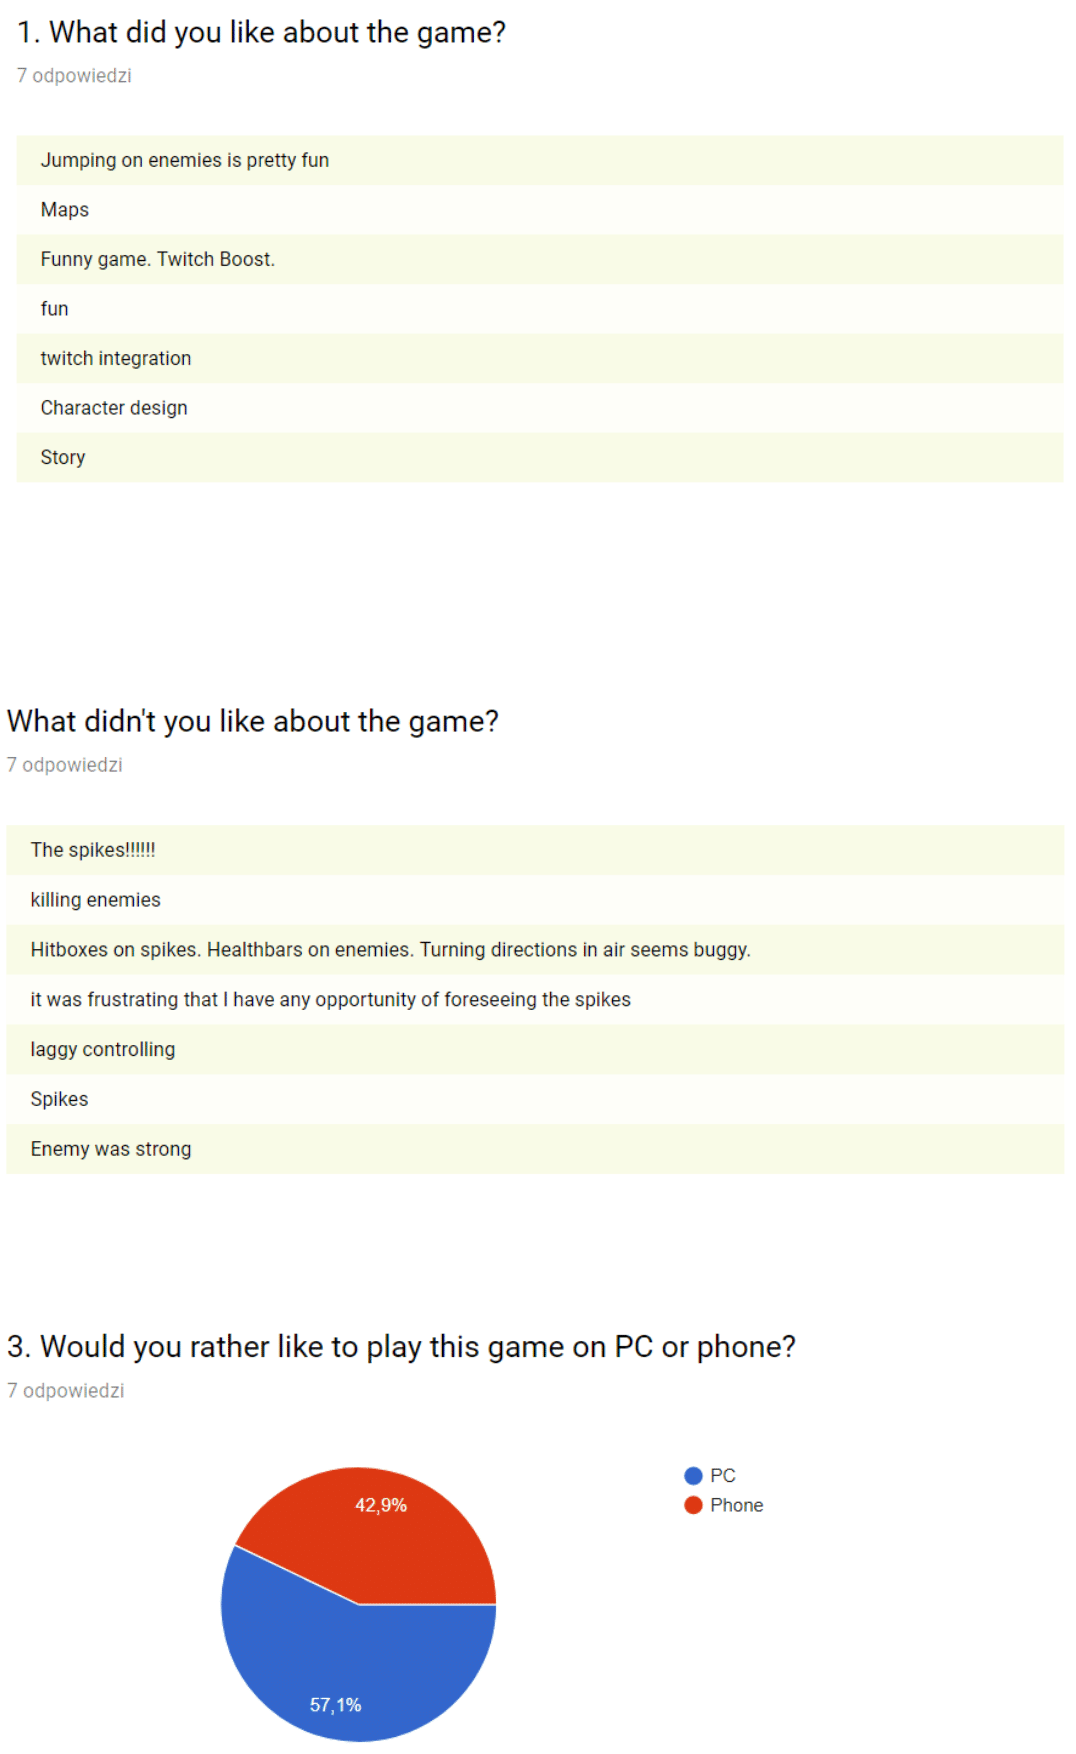
\includegraphics[width=\textwidth,height=\textheight,keepaspectratio]{surveyresults1.png}
 \label{fig:survey_results_1}
\end{figure}

\begin{figure}[ht]
 \center
 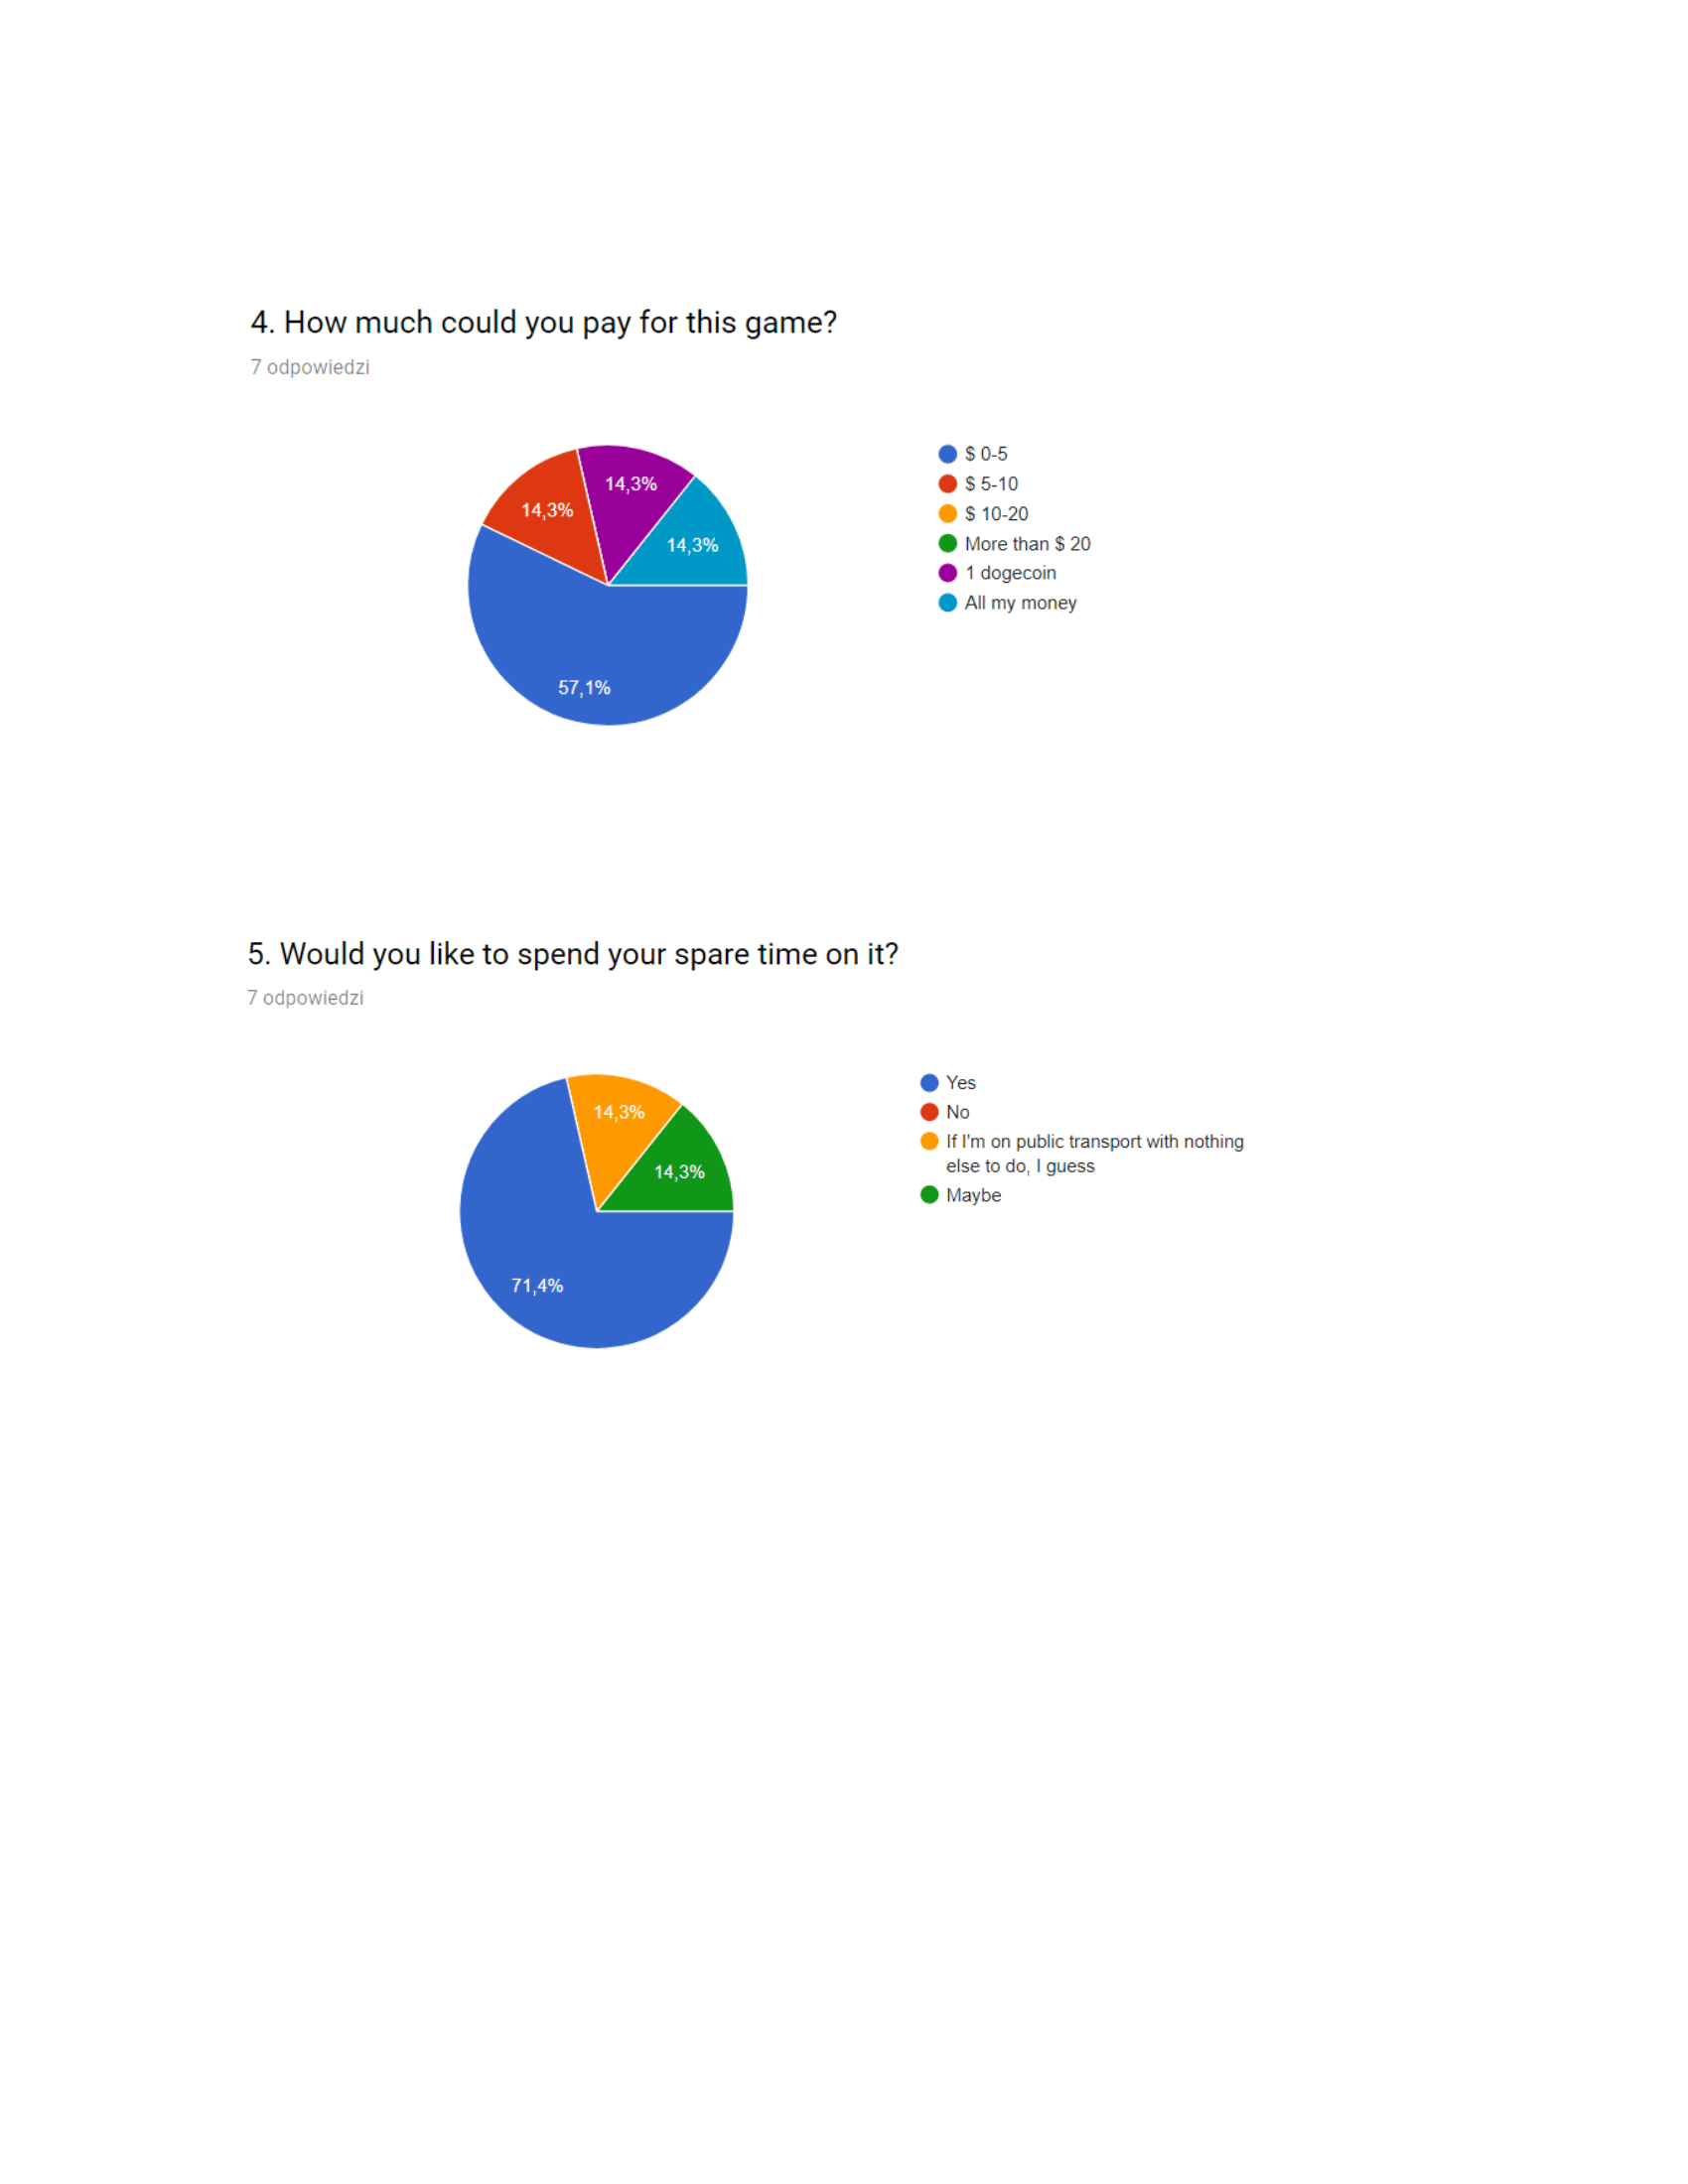
\includegraphics[width=\textwidth,height=\textheight,keepaspectratio]{surveyresults2.png}
 \label{fig:survey_results_2}
\end{figure}

%------------------------------------------------

\end{document}